% Engram: ICLR 2027 submission build (double-blind by default).
% Build (from paper/):  pdflatex main; bibtex main; pdflatex main; pdflatex main
% Camera-ready / named build:  pdflatex "\def\FINAL{}% Engram: ICLR 2027 submission build (double-blind by default).
% Build (from paper/):  pdflatex main; bibtex main; pdflatex main; pdflatex main
% Camera-ready / named build:  pdflatex "\def\FINAL{}% Engram: ICLR 2027 submission build (double-blind by default).
% Build (from paper/):  pdflatex main; bibtex main; pdflatex main; pdflatex main
% Camera-ready / named build:  pdflatex "\def\FINAL{}% Engram: ICLR 2027 submission build (double-blind by default).
% Build (from paper/):  pdflatex main; bibtex main; pdflatex main; pdflatex main
% Camera-ready / named build:  pdflatex "\def\FINAL{}\input{main}"  (then bibtex main; pdflatex x2)
\documentclass{article}
\pdfoutput=1 % force pdfLaTeX (the figures are included as PDF)

% Fallback for TeX installs that lack the `helvetic' package: the ICLR style loads Helvetica-Bold (phvb)
% only for the grey reviewer line-number ruler. `texfonts.map' next to this file aliases phvb -> ptmb
% (Times Bold metrics) when phvb.tfm is missing, and this map line gives pdfTeX the matching glyphs.
% On a complete TeX Live the real phvb.tfm is found first and pdfTeX ignores the duplicate map entry.
\pdfmapline{+phvb NimbusRomNo9L-Medi <utmb8a.pfb}

\usepackage{iclr2027/iclr2027_conference,times}
% \iclrfinalcopy is the camera-ready switch: it prints the author block and the "Published as..." header.
% Default is the anonymous submission build; pass \def\FINAL{} on the command line for the named build.
\ifdefined\FINAL\iclrfinalcopy\fi

\usepackage[utf8]{inputenc}
\usepackage[T1]{fontenc}
\usepackage{amsmath,amssymb}
\usepackage{booktabs}
\usepackage{graphicx}
\usepackage{xcolor}
\usepackage{microtype}
\usepackage[colorlinks=true,linkcolor=black,citecolor=blue!50!black,urlcolor=blue!50!black]{hyperref}
\usepackage{url}
\usepackage{tikz}
\usetikzlibrary{arrows.meta,positioning,fit,backgrounds,shapes.geometric,calc}
\graphicspath{{figs/}}
\usepackage{listings}
\lstdefinestyle{prompt}{%
  basicstyle=\ttfamily\scriptsize, breaklines=true, breakautoindent=false,
  columns=fullflexible, keepspaces=true, showstringspaces=false,
  frame=single, framesep=3pt, xleftmargin=3pt, xrightmargin=3pt, aboveskip=5pt, belowskip=5pt}

% ---- shared figure colors / styles ----
\definecolor{engramblue}{HTML}{1F5C8B}
\definecolor{engramlight}{HTML}{9BB7D4}
\definecolor{baselinered}{HTML}{B0413E}
\definecolor{s2green}{HTML}{2E7D5B}

\newcommand{\engram}{\textsc{Engram}}
\newcommand{\lean}{\texttt{engram\_lean}}
\newcommand{\full}{\texttt{full\_context}}

% Anonymity follows the ICLR switch: the submission build (\iclrfinalfalse) carries no author names,
% affiliations, acknowledgements or self-identifying URLs; \ifanon guards every such string in the body.
\newif\ifanon \ificlrfinal\anonfalse\else\anontrue\fi

\title{Less Context, More Accuracy:\\
A Bi-Temporal Memory Engine for LLM Agents\\
Where a Lean Retrieved Context Beats the Full History}

% The style file prints "Anonymous authors / Paper under double-blind review" unless \iclrfinalcopy is
% set, so the block below is typeset only in the camera-ready build.
\ifanon
\author{Anonymous authors}
\else
\author{%
  Liuyin Wang\thanks{Correspondence: \texttt{liuyinwangthu@gmail.com}. Code, raw logs, and the
  reproducible harness: \url{https://github.com/ly-wang19/engram}.}\\
  Independent Researcher%
}
\fi

\begin{document}
\maketitle
% The style sets the running header inside \maketitle's group with fancyhdr's \lhead. The fancyhdr the
% style file bundles (v3.2) makes that global; fancyhdr >= 4 (any current TeX Live) does not, and the
% header vanishes. Re-issue it here, outside the group, with the style's own wording for both builds.
\ificlrfinal\lhead{Published as a conference paper at ICLR 2027}\else\lhead{Under review as a conference paper at ICLR 2027}\fi

\begin{abstract}
Long-term memory is the missing layer for LLM agents: across sessions they forget, and the common
workaround---replaying the entire history into the prompt---is expensive, slow, and, as distractors
accumulate, \emph{less} accurate. Most memory systems win on cost or latency but still lose to the
full-context baseline on accuracy, and the field's benchmark numbers are reported on inconsistent,
non-reproducible harnesses, so the same system appears at wildly different scores across sources.
We present \engram{}, an open-source, dual-process memory engine built on a bi-temporal data model. A fast
write path appends lossless episodes without an LLM on the critical path; an asynchronous consolidation
path extracts atomic $(\textit{subject},\textit{predicate},\textit{object})$ facts, builds a bi-temporal
knowledge graph, and resolves contradictions \emph{without} an LLM call per fact---invalidating, never
deleting, so every fact retains provenance and a supersession chain. A hybrid read path fuses dense, lexical,
graph, and recency/salience signals, applies a point-in-time (``as-of'') temporal filter, and assembles a
compact, provenance-tagged context. On the full 500-question \textsc{LongMemEval}\textsubscript{S} benchmark,
graded with the \emph{official} category-specific judge prompts, \engram{}'s lean configuration---which
answers from a $\sim$7.9k-token retrieved slice, never the full history---scores \textbf{84.4\%} versus
\textbf{78.8\%} for the full-context baseline ($+5.6$ points, McNemar exact $p=0.009$) while using
\textbf{10$\times$ fewer tokens} (7.9k vs.\ 79k), with 0 of 500 questions errored under both systems. The
advantage grows for a weaker reader: with a small answerer the same slice wins by $+12.2$ points. On a
200-item slice of LOCOMO, whose $\sim$16k-token histories leave little for retrieval to remove, the two
tie overall while the lean path wins the adversarial and multi-hop categories. The gain depends on the read
path being \emph{hybrid}: facts alone lose recall; facts plus retrieved raw chunks recover detail. Beyond the
system, we contribute a neutral, in-repo evaluation harness---official judge baked in, full-context baseline
in every table, raw per-question logs published---and document the measurement-integrity pitfalls that
silently distort memory-benchmark numbers. Every number in this paper ships with the command to reproduce it.
\end{abstract}

\section{Introduction}

LLM agents are stateless across sessions. The pragmatic fix---concatenate the whole conversation history into
the prompt---scales badly on three axes at once: token cost grows linearly with history, latency follows, and
accuracy \emph{degrades} as irrelevant turns crowd the window and the model is forced to locate a needle among
distractors~\citep{liu2024lost}. A long-term memory layer that stores, structures, and selectively retrieves
the past is the natural alternative, and a growing body of systems pursues
it~\citep{packer2023memgpt,park2023generative,chhikara2025mem0,rasmussen2025zep,gutierrez2024hipporag};
see \citet{du2026memorysurvey} for a recent (2026) survey.

Two gaps remain wide open. First, \textbf{accuracy}: most memory systems are reported as cheaper or faster
than full-context, but \emph{not more accurate}. Beating full-context \emph{on accuracy}---a precisely
retrieved slice that outperforms the noisy full window---is the harder and more valuable target, because it
turns memory from a cost optimization into a quality improvement. Second, \textbf{reproducibility}: memory
benchmarks are reported on inconsistent harnesses with different ingestion, answer prompts, and judges, so a
single system can appear tens of points apart depending on the source, and different papers give
contradictory orderings. In a field where every number is contested, a neutral harness anyone can re-run is
itself a contribution.

We address both with \engram{}, an open-source memory engine, and its in-repo evaluation harness. Our design
follows a single principle---\emph{a number we cannot reproduce does not exist}---and a composition thesis:
no single mechanism wins, so we compose typed memory, a bi-temporal knowledge graph, multi-signal retrieval
fusion, salience decay, and asynchronous consolidation, and build in the seams between them.

\paragraph{Contributions.}
\begin{enumerate}
  \item \textbf{A dual-process, bi-temporal memory engine} (\S\ref{sec:system}) with cheap, non-destructive
  conflict resolution: a contradicted fact is \emph{invalidated} (with a \texttt{supersedes} chain and full
  provenance), never overwritten, and the common case is resolved with \emph{no} LLM call.
  \item \textbf{The empirical result that a lean retrieved context beats full-context on accuracy}
  (\S\ref{sec:results}): $+5.6$ points (84.4\% vs.\ 78.8\%) at 10$\times$ fewer tokens on the full
  500-question \textsc{LongMemEval}\textsubscript{S} under the official judge prompts\footnote{\label{fn:judge}%
  The arXiv~v1 of this paper reported 83.6\% vs.\ 73.2\% ($+10.4$) at 9.6k vs.\ 79k tokens on the same % arxiv-v1
  500 questions. That run was graded by a DeepSeek-V3.2 judge served through a third-party endpoint that % arxiv-v1
  has since been retired (the model id now returns \texttt{NotFound}), so it can no longer be re-run. % arxiv-v1
  Every number in this version comes from a fresh full-set run of the current code with the judge moved % arxiv-v1
  to DeepSeek's official API (\S\ref{sec:setup}). The judge is what moved the absolute scores: the % arxiv-v1
  unchanged full-context baseline scored 73.2\% and 76.0\% in two full-set runs under the retired judge % arxiv-v1
  and 77.6\%, 77.4\% and 78.8\% in three runs under the current one, while \lean{} moved % arxiv-v1
  83.6\%\,$\rightarrow$\,84.4\%; the gap therefore narrowed from $+10.4$ to $+5.6$. The reproduce % arxiv-v1
  command in \S\ref{sec:setup} targets the current judge; both logs stay committed.}---i.e.\ removing % arxiv-v1
  distractors \emph{raises} accuracy---and the margin widens to $+12.2$ for a small answerer
  (\S\ref{sec:backbones}), together with the finding that a \emph{hybrid} facts-plus-chunks read path is
  load-bearing (facts alone lose recall).
  \item \textbf{A neutral, reproducible harness} (\S\ref{sec:setup}): one in-repo pipeline with the official
  judge baked in, the full-context baseline in every table, the same answerer and judge applied to every
  system by construction, and the raw per-question logs published. We additionally document the
  measurement-integrity pitfalls we found and fixed.
  \item \textbf{A per-category and cross-backbone analysis} (\S\ref{sec:results}) isolating where the lean
  slice wins (multi-session $+11.3$, single-session-preference $+30.0$, single-session-user $+8.6$) and
  where it loses (knowledge-update $-6.4$), plus a second benchmark---a labelled 200-item LOCOMO
  slice (\S\ref{sec:locomo})---that gives independent evidence for the abstention gate and the multi-hop
  planner and exposes a date-granularity limitation of fact extraction.
\end{enumerate}

\section{Related Work}

\paragraph{Memory systems for LLM agents.}
MemGPT~\citep{packer2023memgpt} frames the LLM as an operating system that pages memory in and out of a
limited context window. Generative Agents~\citep{park2023generative} introduce a memory stream with
importance, recency, and relevance scoring plus periodic reflection. Mem0~\citep{chhikara2025mem0} targets
production agents with scalable extract-and-store memory. Zep/Graphiti~\citep{rasmussen2025zep} is the closest
in spirit to \engram{}: a temporally-aware knowledge-graph memory with bi-temporal edges.
HippoRAG~\citep{gutierrez2024hipporag} uses a graph plus personalized PageRank for multi-hop retrieval, and
its successor HippoRAG~2~\citep{gutierrez2025hipporag2} reframes the same machinery as non-parametric continual
memory. The most recent agentic-memory systems add LLM-driven control over how memories are written and
organized: A-MEM~\citep{xu2025amem} builds an interlinked, Zettelkasten-style note network;
MemoryOS~\citep{kang2025memoryos} imposes an operating-system-style short/mid/long-term hierarchy; and
GAM~\citep{wu2026gam} decouples memory encoding from consolidation over hierarchical graphs. \engram{} differs in
\emph{composing} a bi-temporal graph with a hybrid (facts + raw chunks) read path and an explicit, cheap
conflict-resolution policy, and---distinctively---in shipping the neutral harness that lets these design
choices be measured rather than asserted.

\paragraph{Long context and the cost of distractors.}
``Lost in the middle''~\citep{liu2024lost} shows that LLMs use long contexts unevenly and that accuracy
degrades when relevant evidence is buried among distractors. This is the mechanism our headline result
exploits: a filtered, precisely retrieved slice can be \emph{more} accurate than the full window, not merely
cheaper.

\paragraph{Benchmarks.}
\textsc{LongMemEval}~\citep{wu2025longmemeval} evaluates chat assistants on long-term interactive memory
across categories (single/multi-session, knowledge-update, temporal reasoning, preference, and abstention),
with category-specific judge prompts. LOCOMO~\citep{maharana2024locomo} evaluates very long-term
conversational memory, and more recent benchmarks extend the setting to multimodal histories
(Mem-Gallery~\citep{bei2026memgallery}). We report on \textsc{LongMemEval}\textsubscript{S} with two answerer
backbones and on a 200-item LOCOMO slice (\S\ref{sec:locomo}); the full LOCOMO set is in progress
(\S\ref{sec:limitations}).

\paragraph{Retrieval.}
\engram{}'s read path builds on dense retrieval~\citep{karpukhin2020dpr} with modern dense sentence
embeddings (the BGE family~\citep{xiao2024cpack}; we use the English \texttt{bge-small-en-v1.5}), classical
lexical scoring (BM25~\citep{robertson2009bm25}), and Reciprocal Rank Fusion~\citep{cormack2009rrf}, in
the retrieval-augmented generation tradition~\citep{lewis2020rag}. The dual-process framing draws on the System-1/System-2 distinction in
cognitive science~\citep{kahneman2011thinking}, and salience decay on the classical forgetting
curve~\citep{ebbinghaus1913memory}.

\section{The \engram{} System}
\label{sec:system}

\engram{} is a dual-process memory system: a fast online write path (System-1) and a slow asynchronous
consolidation path (System-2) that writes into a typed, bi-temporal memory, which a hybrid read path queries
(Figure~\ref{fig:arch}).

\begin{figure}[t]
\centering
\resizebox{0.84\textwidth}{!}{%
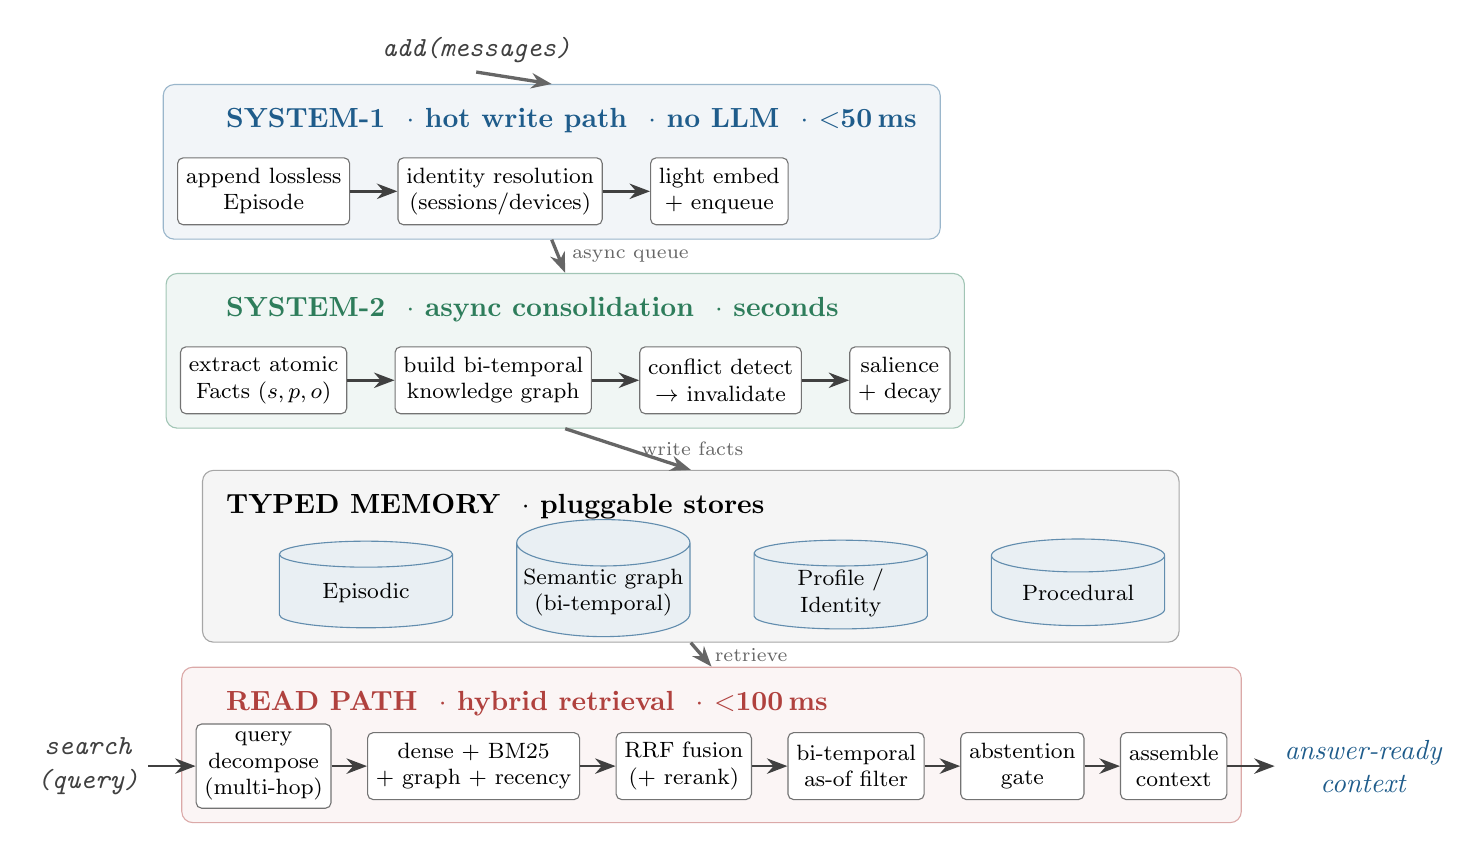
\begin{tikzpicture}[
  font=\footnotesize,
  chip/.style={rounded corners=2pt, draw=black!55, fill=white, inner sep=3pt,
               minimum height=8.5mm, align=center},
  store/.style={cylinder, shape border rotate=90, aspect=0.28, draw=engramblue!70,
                fill=engramblue!10, minimum height=11mm, minimum width=22mm, align=center,
                inner sep=1pt},
  io/.style={font=\itshape, text=black!75, align=center},
  ttl/.style={font=\bfseries, anchor=west},
  >={Stealth[length=2.6mm]},
  flow/.style={->, line width=1pt, draw=black!75},
  vflow/.style={->, line width=1.2pt, draw=black!60},
]
% ----- input -----
\node[io] (in) at (3.0,10.2) {\texttt{add(messages)}};
% ----- SYSTEM-1 -----
\node[ttl, text=engramblue] (t1) at (-0.3,9.3) {SYSTEM-1 \ $\cdot$\ hot write path \ $\cdot$\ no LLM \ $\cdot$\ $<$50\,ms};
\node[chip] (s1a) at (0.3,8.4) {append lossless\\Episode};
\node[chip, right=6mm of s1a] (s1b) {identity resolution\\(sessions/devices)};
\node[chip, right=6mm of s1b] (s1c) {light embed\\$+$ enqueue};
\draw[flow] (s1a)--(s1b); \draw[flow] (s1b)--(s1c);
% ----- SYSTEM-2 -----
\node[ttl, text=s2green] (t2) at (-0.3,6.9) {SYSTEM-2 \ $\cdot$\ async consolidation \ $\cdot$\ seconds};
\node[chip] (s2a) at (0.3,6.0) {extract atomic\\Facts $(s,p,o)$};
\node[chip, right=6mm of s2a] (s2b) {build bi-temporal\\knowledge graph};
\node[chip, right=6mm of s2b] (s2c) {conflict detect\\$\to$ invalidate};
\node[chip, right=6mm of s2c] (s2d) {salience\\$+$ decay};
\draw[flow] (s2a)--(s2b); \draw[flow] (s2b)--(s2c); \draw[flow] (s2c)--(s2d);
% ----- TYPED MEMORY -----
\node[ttl] (t3) at (-0.3,4.4) {TYPED MEMORY \ $\cdot$\ pluggable stores};
\node[store] (m1) at (1.6,3.3) {Episodic};
\node[store, right=8mm of m1] (m2) {Semantic graph\\(bi-temporal)};
\node[store, right=8mm of m2] (m3) {Profile /\\Identity};
\node[store, right=8mm of m3] (m4) {Procedural};
% ----- READ PATH -----
\node[ttl, text=baselinered] (t4) at (-0.3,1.9) {READ PATH \ $\cdot$\ hybrid retrieval \ $\cdot$\ $<$100\,ms};
\node[chip] (r1) at (0.3,1.1) {query\\decompose\\(multi-hop)};
\node[chip, right=4.5mm of r1] (r2) {dense $+$ BM25\\$+$ graph $+$ recency};
\node[chip, right=4.5mm of r2] (r3) {RRF fusion\\($+$ rerank)};
\node[chip, right=4.5mm of r3] (r4) {bi-temporal\\as-of filter};
\node[chip, right=4.5mm of r4] (r5) {abstention\\gate};
\node[chip, right=4.5mm of r5] (r6) {assemble\\context};
\draw[flow] (r1)--(r2); \draw[flow] (r2)--(r3); \draw[flow] (r3)--(r4);
\draw[flow] (r4)--(r5); \draw[flow] (r5)--(r6);
\node[io, left=6mm of r1] (q) {\texttt{search}\\\texttt{(query)}};
\draw[flow] (q)--(r1);
\node[io, right=6mm of r6, text=engramblue] (out) {answer-ready\\context};
\draw[flow] (r6)--(out);
% ----- background bands -----
\begin{scope}[on background layer]
\node[rounded corners=4pt, fill=engramblue!6, draw=engramblue!45, fit=(t1)(s1a)(s1c), inner sep=5pt] (bandS1) {};
\node[rounded corners=4pt, fill=s2green!7, draw=s2green!45, fit=(t2)(s2a)(s2d), inner sep=5pt] (bandS2) {};
\node[rounded corners=4pt, fill=black!4, draw=black!35, fit=(t3)(m1)(m4), inner sep=5pt] (bandM) {};
\node[rounded corners=4pt, fill=baselinered!5, draw=baselinered!45, fit=(t4)(r1)(r6), inner sep=5pt] (bandR) {};
\end{scope}
% ----- vertical flow between bands -----
\draw[vflow] (in.south)--(bandS1.north);
\draw[vflow] (bandS1.south)--node[right=1pt,font=\scriptsize,text=black!60]{async queue}(bandS2.north);
\draw[vflow] (bandS2.south)--node[right=1pt,font=\scriptsize,text=black!60]{write facts}(bandM.north);
\draw[vflow] (bandM.south)--node[right=1pt,font=\scriptsize,text=black!60]{retrieve}(bandR.north);
\end{tikzpicture}%
}
\caption{The \engram{} dual-process architecture: a hot write path (\textsc{System-1}) that never blocks on
an LLM; an asynchronous consolidation path (\textsc{System-2}) that extracts facts, builds the bi-temporal
graph and resolves conflicts non-destructively; a typed memory over pluggable stores; and a hybrid read path
(dense $+$ lexical $+$ graph $+$ recency, fused by RRF) with an as-of filter and an abstention gate.}
\label{fig:arch}
\end{figure}

\subsection{Bi-temporal data model}

Two time axes are first-class everywhere, which is what makes knowledge-updates and ``as-of'' queries
intrinsic rather than bolted-on.

\begin{itemize}
  \item \textbf{Episode} --- a raw, lossless turn/event, stamped with \emph{event time} (when it happened in
  the world) and \emph{ingested-at} (transaction time, when we recorded it).
  \item \textbf{Fact} --- an atomic $(\textit{subject},\textit{predicate},\textit{object})$ claim with surface
  text, an embedding, a \emph{salience} and \emph{confidence}, and \emph{provenance} (the source episode
  ids). It carries two time axes: \emph{valid time} (\texttt{valid\_at} / \texttt{invalid\_at}, when the claim
  is true in the world) and \emph{transaction time} (\texttt{created\_at} / \texttt{expired\_at}, when we
  learned or retracted it), plus a \texttt{supersedes} pointer to the fact it replaces.
  \item \textbf{Entity / Relation} --- graph nodes and edges; edges carry the same bi-temporal stamps.
\end{itemize}

The invariant: \emph{never hard-delete a contradicted fact---invalidate it} (set \texttt{invalid\_at}) and
keep the history. Every fact can therefore answer ``where did this come from?'' and ``what did it replace?''
(Figure~\ref{fig:bitemporal}).

\begin{figure}[t]
\centering
\resizebox{0.8\textwidth}{!}{%
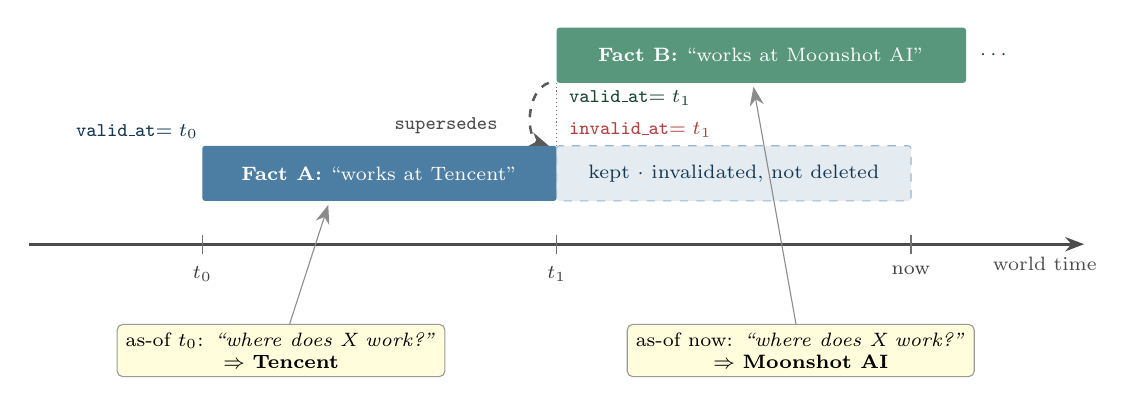
\begin{tikzpicture}[font=\footnotesize, >={Stealth[length=2.4mm]}]
% time axis
\draw[->, line width=1pt, black!70] (-0.2,0)--(13.2,0);
\node[font=\scriptsize, text=black!70, below] at (12.7,-0.04) {world time};
\foreach \x/\lab in {2/{$t_0$}, 6.5/{$t_1$}, 11/{now}}{
  \draw[black!55] (\x,0.12)--(\x,-0.12);
  \node[below, font=\scriptsize, text=black!75] at (\x,-0.16) {\lab};
}
% Fact A: valid in [t0,t1)
\fill[engramblue!80, rounded corners=1pt] (2,0.55) rectangle (6.5,1.25);
\node[white, font=\scriptsize] at (4.25,0.9) {\textbf{Fact A:} ``works at Tencent''};
% Fact A kept-but-invalid in [t1, now]
\draw[fill=engramblue!12, draw=engramblue!45, dashed, rounded corners=1pt] (6.5,0.55) rectangle (11,1.25);
\node[text=engramblue!60!black, font=\scriptsize] at (8.75,0.9) {kept $\cdot$ invalidated, not deleted};
\node[font=\scriptsize, text=engramblue!60!black, above left=-1pt and -2pt] at (2,1.25) {\texttt{valid\_at}$=t_0$};
% Fact B: valid in [t1, ...)
\fill[s2green!80, rounded corners=1pt] (6.5,2.05) rectangle (11.7,2.75);
\node[white, font=\scriptsize] at (9.1,2.4) {\textbf{Fact B:} ``works at Moonshot AI''};
\node[text=s2green!55!black, font=\scriptsize, right] at (11.75,2.4) {$\cdots$};
% supersession instant at t1
\draw[densely dotted, black!55] (6.5,1.25)--(6.5,2.05);
\node[font=\scriptsize, text=baselinered, right=1pt] at (6.5,1.45) {\texttt{invalid\_at}$=t_1$};
\node[font=\scriptsize, text=s2green!55!black, right=1pt] at (6.5,1.86) {\texttt{valid\_at}$=t_1$};
% supersedes arrow B -> A (bowing left of t1)
\draw[->, dashed, line width=0.9pt, black!65] (6.4,2.05) to[out=-160,in=160] (6.4,1.25);
\node[font=\scriptsize, text=black!70, left=5pt] at (6.05,1.5) {\texttt{supersedes}};
% as-of queries
\node[rounded corners=2pt, draw=black!40, fill=yellow!14, font=\scriptsize, align=center, inner sep=3pt]
  (qa) at (3,-1.35) {as-of $t_0$: \emph{``where does X work?''}\\$\Rightarrow$ \textbf{Tencent}};
\node[rounded corners=2pt, draw=black!40, fill=yellow!14, font=\scriptsize, align=center, inner sep=3pt]
  (qb) at (9.6,-1.35) {as-of now: \emph{``where does X work?''}\\$\Rightarrow$ \textbf{Moonshot AI}};
\draw[->, black!45] (qa)--(3.6,0.5);
\draw[->, black!45] (qb)--(9.0,2.0);
\end{tikzpicture}%
}
\caption{Bi-temporal facts make contradictions and ``as-of'' queries first-class: when Fact~B arrives at
$t_1$, \engram{} sets $\text{A.}\texttt{invalid\_at}=t_1$ and $\text{B.}\texttt{supersedes}=\text{A}$---A is
\emph{invalidated, not deleted}, so history and provenance survive---and a point-in-time query resolves
against the fact valid at that time, which is what the knowledge-update and temporal categories require.}
\label{fig:bitemporal}
\end{figure}

\subsection{System-1: the hot write path}

On \texttt{add(messages)}, \engram{} appends a lossless episode, resolves identity (linking a user/entity
across sessions and devices), computes a light embedding, and enqueues the episode for consolidation. No LLM
runs on this path, keeping it within a sub-50ms budget so writes never block the agent.

\subsection{System-2: asynchronous consolidation}

Off the critical path, the consolidation engine (i) extracts atomic facts from episodes (rule-based by
default, LLM-based when a model is configured), (ii) builds the bi-temporal knowledge graph of entities and
relations, (iii) detects conflicts and invalidates superseded facts, and (iv) scores salience and applies
decay/reinforcement so unreinforced memories fade and the store stays small and fast. Hierarchical
abstraction (session summaries $\rightarrow$ profile) runs here as well.

\subsection{Cheap-then-escalate conflict resolution}

When a new fact arrives for an existing $(\textit{subject},\textit{predicate})$ slot with a different object,
\engram{} resolves it in increasing order of cost. First, cheap signals: an exact \textbf{slot match}
signals a likely update, \textbf{embedding similarity} catches the same attribute under a different
free-form predicate, and \textbf{content subsumption} (one claim $\subseteq$ the other) separates
contradiction from elaboration. Second, if the claims are clearly contradictory and temporally ordered, the
old one is invalidated ($\texttt{old.invalid\_at} \leftarrow \texttt{new.valid\_at}$) and
$\texttt{new.supersedes} \leftarrow \texttt{old.id}$---with \emph{no LLM call}. Only genuinely ambiguous cases
escalate to an LLM adjudicator. This is the cost win over systems that invoke an LLM on every fact, while
preserving temporal correctness and a complete audit trail.

\subsection{The hybrid read path}

On \texttt{search(query)}, \engram{} (1) understands the query and, for multi-hop questions, decomposes it
into sub-queries; (2) retrieves in parallel through four complementary channels---dense semantic, BM25
lexical, graph $n$-hop from the query's entities, and recency/salience; (3) fuses the ranked lists with
Reciprocal Rank Fusion~\citep{cormack2009rrf} and an optional cross-encoder rerank over the top-$k$ (off by
default); (4) applies a bi-temporal ``as-of'' filter (what we believed was true at time $T$); (5) passes an
abstention gate that declines to answer when the evidence is absent; and (6) assembles a deduplicated,
provenance-tagged, token-budgeted context. The per-item score combines all signals:
\begin{equation}
\label{eq:score}
\begin{split}
\mathrm{score}(\textit{item} \mid q) ={}&
  w_{\text{sem}}\cos(q,\textit{item})
  + w_{\text{lex}}\,\mathrm{bm25}(q,\textit{item})
  + w_{\text{graph}}\,\mathrm{prox}(\textit{item}) \\
  &{}+ w_{\text{rec}}\,e^{-\Delta t/\tau}
  + w_{\text{sal}}\,\mathrm{sal}(\textit{item}),
\end{split}
\end{equation}
where the weights are configuration-driven and tuned on the harness rather than hand-set. Crucially, the
assembled context is \emph{hybrid}: it contains both the conflict-resolved bi-temporal facts and the most
relevant raw session chunks (plus session-level summaries). \S\ref{sec:results} shows this hybrid composition
is necessary---facts alone lose recall.

Every external dependency---LLM, embedder, vector, graph and lexical store---sits behind an interface with
a zero-dependency offline fallback, so the loop runs with no API keys (Appendix~\ref{app:backends}).

\section{Experimental Setup}
\label{sec:setup}

\paragraph{Benchmark.}
\textsc{LongMemEval}\textsubscript{S}~\citep{wu2025longmemeval}: 500 questions, each over a haystack of
$\sim$50 sessions ($\sim$115k tokens), pulled from the public release. Questions span seven categories
(Figure~\ref{fig:percat}). We grade with the \emph{official} category-specific judge prompts---including the
temporal off-by-one tolerance, knowledge-update old-information tolerance, preference-rubric leniency, the
``contains the answer'' semantics, and unanswerable (abstention) detection---rather than a home-grown judge.

\paragraph{Models.}
Embedder: \texttt{BAAI/bge-small-en-v1.5} (local, no API key). System-2 fact extractor:
\texttt{doubao-seed-1.6-flash}. Answerer: \texttt{doubao-seed-2.0-pro} for the headline, and the small
\texttt{doubao-seed-1.6-flash} as a second backbone (\S\ref{sec:backbones}). Judge: DeepSeek's official API
(\texttt{deepseek-chat}, which served DeepSeek-V4-Flash at the time of the runs), prompted with the official
LongMemEval judge prompts; footnote~\ref{fn:judge} explains why this differs from the arXiv~v1 judge. Models
are addressed as \texttt{provider:model} and resolved via LiteLLM, so any OpenAI-compatible endpoint (OpenAI,
DeepSeek, a local model) can be substituted and the same commands run.

\paragraph{Systems.}
\lean{} (our headline) retrieves a small hybrid slice---conflict-resolved bi-temporal facts $+$ the most
relevant raw session chunks $+$ session summaries---and answers from \emph{that alone} ($\sim$7.9k tokens),
never the full history. \full{} is the baseline: stuff the entire haystack into the prompt ($\sim$79k tokens).
The harness applies the \emph{same answerer and judge to every system}, so any within-run comparison is
apples-to-apples by construction.

\paragraph{Retrieval configuration.}
The hybrid read path fuses five ranked signals by weighted Reciprocal Rank Fusion ($k_{\text{RRF}}=60$) with
the Eq.~\eqref{eq:score} weights $w_{\text{sem}}=1.0$, $w_{\text{lex}}=0.6$, $w_{\text{graph}}=0.8$,
$w_{\text{rec}}=0.3$, $w_{\text{sal}}=0.25$ (the repository defaults in \texttt{engram/config.py}, tuned on
the harness, not hand-set per question). The lean slice assembles up to 8 conflict-resolved facts, the
top-15 fused items, 2 raw session chunks, and 28 session-level summaries; exact flag semantics are in the
reproduce command.

\paragraph{Reproduce.}
The headline run is a single command, given verbatim (with the model identifiers and every flag) in the
Reproducibility Statement; its raw per-question log is committed to the repository as
\texttt{results/run500\_v3\_main\_deepseekjudge.jsonl}. The second backbone swaps the answerer flag and the
LOCOMO slice the data flag, nothing else. \texttt{python eval/report.py <run.jsonl>} recomputes every table
below from a log, and \texttt{python paper/check\_numbers.py} asserts that every number in this paper's
main text equals a value recomputed from the committed logs.

\paragraph{Measurement-integrity notes.}
Six bugs and drifts that silently inflate or deflate memory-benchmark numbers---and that we hit and fixed
ourselves---are documented in Appendix~\ref{app:integrity}: a ``memory'' system that still contained the
full history, a truncated full-context baseline, a home-grown judge stricter than the official one,
abstention grading, retry handling (the headline run has 0 errored questions of 500 under both systems),
and the judge-endpoint drift of footnote~\ref{fn:judge}. They are the reason cross-source numbers disagree.

\section{Results}
\label{sec:results}

\paragraph{Headline.}
Table~\ref{tab:headline} and Figure~\ref{fig:acctokens} report the full 500-question result. \engram{}'s lean
configuration beats the full-context baseline by \textbf{$+5.6$ points} (84.4\% vs.\ 78.8\%) while using
\textbf{10$\times$ fewer tokens} (7.9k vs.\ 79k), with 0 of 500 errored under both. The filtered slice is not
merely cheaper---it is \emph{more accurate} than the full window, consistent with the distractor mechanism
of \citet{liu2024lost}. The margin is statistically significant but not large: across the 500 paired
questions \lean{} is correct on 68 that the baseline misses versus 40 the other way (McNemar's exact test,
$p=0.009$), and a paired bootstrap puts the 95\% CI of the gain at $+1.6$ to $+9.6$ points. All statistics
are recomputed from the committed log by \texttt{paper/compute\_stats.py}.

\begin{table}[h]
\centering
\caption{\textsc{LongMemEval}\textsubscript{S}, 500 questions, official judge prompts; same answerer
(\texttt{doubao-seed-2.0-pro}) and judge (\texttt{deepseek-chat}) for both systems. Accuracy with a Wilson
95\% CI (paired difference: McNemar exact $p=0.009$); latency is end-to-end wall-clock per question
including the remote answerer call, p50\,/\,p95.}
\label{tab:headline}
\resizebox{\linewidth}{!}{%
\begin{tabular}{lcrrr}
\toprule
System & Overall acc.\ (95\% CI) & Avg.\ context tokens & Latency p50\,/\,p95 & Errors \\
\midrule
\textbf{\engram{}} (\lean{}) & \textbf{84.4\%} \,[81.0,\,87.3] & \textbf{7.9k} & 52.9\,s\,/\,118.7\,s & 0 / 500 \\
full-context baseline        & 78.8\% \,[75.0,\,82.2]          & 79.2k         & 14.6\,s\,/\,59.2\,s  & 0 / 500 \\
\bottomrule
\end{tabular}}
\end{table}

\begin{figure}[t]
\centering
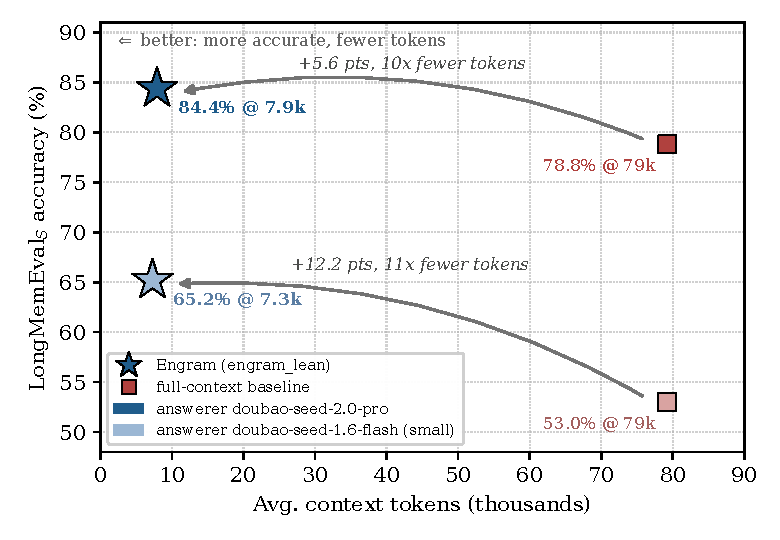
\includegraphics[width=0.62\textwidth]{fig_acc_tokens.pdf}
\caption{Accuracy vs.\ average context tokens on LongMemEval\textsubscript{S} (500 questions) for two answerer
backbones: \lean{} (star) sits up and to the left of full-context (square)---\textbf{$+5.6$ points at
10$\times$ fewer tokens} for \texttt{doubao-seed-2.0-pro}, $+12.2$ at 11$\times$ for the small
\texttt{doubao-seed-1.6-flash} (Table~\ref{tab:backbones}).}
\label{fig:acctokens}
\end{figure}

\paragraph{Per-category.}
Table~\ref{tab:percat} and Figure~\ref{fig:percat} break both systems down by category. The lean slice wins
four of the six categories and ties one. The margins are largest where the full window has the most to
distract from: \emph{single-session-preference} ($+30.0$; a category that is hard field-wide, and where the
baseline reaches only 50.0\%), \emph{multi-session} aggregation ($+11.3$; counting and aggregating across
many sessions, where the baseline mostly abstains) and \emph{single-session-user} ($+8.6$).
\emph{Temporal-reasoning} (date-stamped context $+$ as-of filtering) is a modest $+2.3$. The one loss is
\emph{knowledge-update} ($-6.4$): the baseline sees every version of a changed value in order and applies
``most recent wins'' itself, whereas the lean slice depends on consolidation having attached the update to
the right slot. Of the eight knowledge-update questions the slice loses and the baseline gets, seven end in
a superseded value or an abstention---consistent with the update not reaching the slice, a consolidation
miss rather than a reading error (\S\ref{sec:limitations}). The 30 \emph{abstention} items, graded by the
official \emph{unanswerable} judge and counted inside their host categories above, come out at 90.0\% for
\lean{} vs.\ 93.3\% for the baseline: the abstention gate declines correctly on most of them, at a small
cost against a baseline that, as the error analysis below shows, abstains often anyway.

\begin{table}[h]
\centering\footnotesize
\caption{Per-category accuracy on \textsc{LongMemEval}\textsubscript{S} (500 questions; the run of
Table~\ref{tab:headline}). $\Delta$ is \lean{} minus full-context. The 30 unanswerable (abstention) items are
counted inside their host categories; broken out, they score 90.0\% (\lean{}) vs.\ 93.3\% (full-context).}
\label{tab:percat}
\begin{tabular}{lrrrr}
\toprule
Category & \lean{} & full-context & $\Delta$ & $n$ \\
\midrule
multi-session             & \textbf{78.2\%} & 66.9\%          & $+11.3$ & 133 \\
temporal-reasoning        & \textbf{83.5\%} & 81.2\%          & $+2.3$  & 133 \\
knowledge-update          & 84.6\%          & \textbf{91.0\%} & $-6.4$  & 78 \\
single-session-user       & \textbf{91.4\%} & 82.9\%          & $+8.6$  & 70 \\
single-session-assistant  & 94.6\%          & 94.6\%          & $+0.0$  & 56 \\
single-session-preference & \textbf{80.0\%} & 50.0\%          & $+30.0$ & 30 \\
\midrule
overall                   & \textbf{84.4\%} & 78.8\%          & $+5.6$  & 500 \\
\bottomrule
\end{tabular}
\end{table}

\begin{figure}[t]
\centering
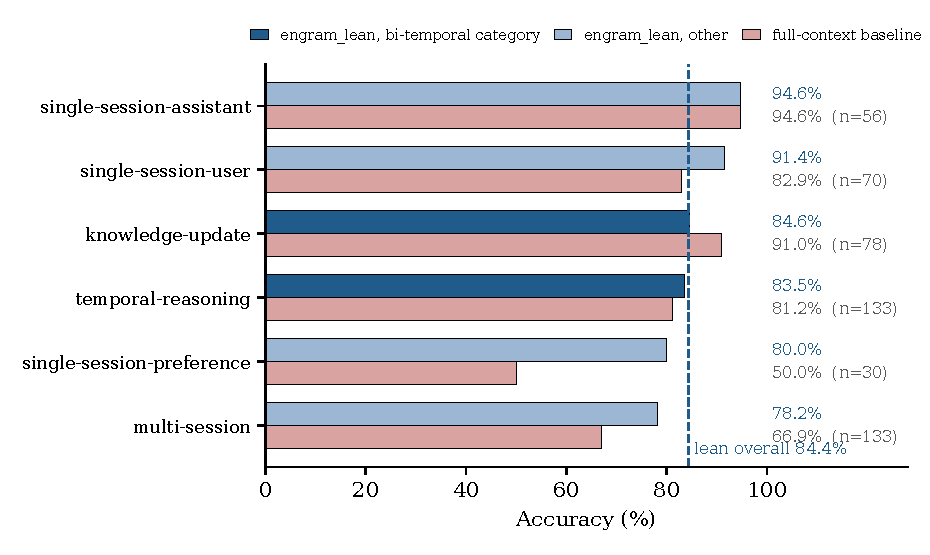
\includegraphics[width=0.74\textwidth]{fig_percat.pdf}
\caption{Per-category accuracy of \lean{} vs.\ full-context on the full 500-question set (dashed line: the
84.4\% lean overall). The two bi-temporal categories are highlighted: temporal-reasoning a small win,
knowledge-update the one loss; the largest margins are single-session-preference and multi-session.}
\label{fig:percat}
\end{figure}

\paragraph{Error analysis: full-context is ``lost in the middle.''}
The two systems fail differently. Of the full-context baseline's 106 errors, \textbf{57\% (60) are
abstentions}---it answers ``I don't know'' even though, by construction, the evidence lies somewhere in its
$\sim$79k-token window; it simply fails to locate it. On the 68 questions where \lean{} is correct and
full-context is wrong, full-context abstains on 59\% (40) and returns a \emph{wrong} value on the other 28.
\lean{}, answering from a $\sim$7.9k-token slice, abstains on 60/500---and 27 of those are among the 30
genuinely unanswerable items. This is the ``lost in the middle'' effect~\citep{liu2024lost} made
quantitative: past a point, more context is \emph{not} more accuracy if the model cannot find the relevant
span (counts recomputed from the committed logs by \texttt{paper/compute\_stats.py}).

\paragraph{The read path must be hybrid.}
A load-bearing finding from development: a \emph{facts-only} read path---answering purely from extracted
$(s,p,o)$ facts---\emph{loses recall} relative to the hybrid path, because extraction drops detail that some
questions need verbatim. Adding the most relevant raw session chunks back alongside the conflict-resolved
facts restores that detail; the facts contribute conflict-resolved, bi-temporal signal and the chunks restore
specificity. The headline configuration is hybrid for exactly this reason, and we caution against shipping
facts-only QA. We report this as a design observation; a controlled facts-only ablation on the full
500-question set under the same judge is reported as future work (\S\ref{sec:limitations}), not claimed here.

\paragraph{Efficiency.}
The retrieved context averages $\sim$7.9k tokens, 10$\times$ leaner than the $\sim$79k full-context
baseline; the saving is in prompt tokens, the quantity that grows with history. End-to-end latency per
question is \emph{higher} for \lean{} (p50 52.9\,s vs.\ 14.6\,s, Table~\ref{tab:headline}). The harness
records wall-clock per question including the remote answerer call and does not instrument retrieval
separately, so we report the latency as measured and make no retrieval-latency claim from these logs.

\subsection{A second backbone: the weaker the reader, the larger the gain}
\label{sec:backbones}

Memory quality should not depend on one model's ability to read our structures, so the same 500 questions
were also run with the answerer swapped for the small \texttt{doubao-seed-1.6-flash}, everything else
unchanged (Table~\ref{tab:backbones}). That run was made in June on the revision of that date and graded by
the judge that has since been retired (footnote~\ref{fn:judge}), so the table names the code revision and
judge per row and we include the June run of the pro answerer as its within-judge sibling; every row is a
within-run, same-judge comparison, which is the claim we make. The lean slice wins under every backbone and
judge, and the margin is \emph{largest for the weakest reader}: $+12.2$ points (65.2\% vs.\ 53.0\%) for the
small answerer, against $+3.0$ for the pro answerer under the same judge and code, and $+5.6$ on the current
code, at a $\sim$10--11$\times$ token ratio throughout. With the small answerer the lean advantage holds in
five of six categories, the exception being single-session-assistant, which is near ceiling for both
(per-category gaps in Appendix~\ref{app:flash}). The reading is simple: a strong model can partly compensate for a
noisy window by searching it; a weak one cannot, so removing distractors is worth more to it. That is the
regime that matters for cheap and local deployments.

\begin{table}[h]
\centering\small
\caption{Answerer backbones on the same 500 questions, extractor and harness (gap $=$ \lean{} $-$
full-context; token ratio $=$ full-context / lean tokens). Each row is a within-run comparison under one
judge; rows differ in code revision and judge as marked, so compare gaps, not levels, across rows. Logs:
\texttt{run500\_v3\_main\_deepseekjudge}, \texttt{headline\_500}, \texttt{bb\_flash} (\texttt{results/*.jsonl}).}
\label{tab:backbones}
\resizebox{\linewidth}{!}{%
\begin{tabular}{llrrrr}
\toprule
Answerer & Code / judge & \lean{} & full-context & Gap & Token ratio \\
\midrule
\texttt{doubao-seed-2.0-pro}   & current / \texttt{deepseek-chat}    & \textbf{84.4\%} & 78.8\% & $+5.6$  & 10.0$\times$ \\
\texttt{doubao-seed-2.0-pro}   & June 2026 / retired ARK judge & \textbf{79.0\%} & 76.0\% & $+3.0$  & 10.9$\times$ \\
\texttt{doubao-seed-1.6-flash} & June 2026 / retired ARK judge & \textbf{65.2\%} & 53.0\% & $+12.2$ & 10.9$\times$ \\
\bottomrule
\end{tabular}}
\end{table}

\subsection{A second benchmark: a 200-item LOCOMO slice}
\label{sec:locomo}

% TODO(locomo-full): the full 1986-item LOCOMO run (results/locomo1986_main_deepseekjudge.jsonl) is in
% flight. When it lands: repoint LOCOMO_SLICE in compute_stats.py, replace the numbers in this subsection
% and in the abstract/related-work mentions, and drop the "slice" labels.
LOCOMO~\citep{maharana2024locomo} is a different regime: ten long multi-session conversations whose full
text is only $\sim$16k tokens, a fraction of a \textsc{LongMemEval}\textsubscript{S} haystack. We converted
its QA pairs into the harness's item format so that the \emph{same} answerer, extractor and judge apply
(its adversarial questions map onto the unanswerable judge), and report the \textbf{first 200 of its 1,986
items}---a slice, labelled as such; the full run is in progress. Table~\ref{tab:locomo} gives the result.
Overall the two systems tie (88.0\% vs.\ 89.0\%, $-1.0$; 0 errors under both) at 3.4k vs.\ 16.2k tokens
($\sim$5$\times$). That the margin shrinks to zero here is the expected behaviour, not a regression: with a
16k-token history there is little for retrieval to remove and the full-context reader is not yet lost. The
lean advantage is a function of how much distracting history there is---clear on the $\sim$79k-token
\textsc{LongMemEval} windows, nil on 16k---and we expect it to grow, not shrink, with history length.

The per-category split carries the information. Two of \engram{}'s design bets get independent evidence:
\emph{adversarial} (the answer is not in the conversation) is 100.0\% vs.\ 91.1\% ($+8.9$, $n=45$)---the
abstention gate declines correctly on every item, where the full-context reader answers some---and
\emph{multi-hop} is 78.6\% vs.\ 71.4\% ($+7.1$, $n=28$), the category the multi-hop query planner targets
and one \textsc{LongMemEval} has no separate label for. Single-hop is within noise ($-3.6$, $n=83$). The
clear loss is \emph{temporal-reasoning} ($-16.2$, $n=37$), and its failures are not retrieval misses but
\emph{date-granularity} errors: gold answers such as ``the week before 9 June 2023'' or ``the first weekend
of August'' come back as a single collapsed timestamp, off by weeks or a month, because fact extraction
reduces a relative time expression to one point on the axis while the full-context reader still sees the
original phrasing. This is a limitation of the current extractor that \textsc{LongMemEval}'s more regular
date annotations did not expose---the concrete value of a second benchmark---and it is the next target for
the bi-temporal model (\S\ref{sec:limitations}).

\begin{table}[h]
\centering\footnotesize
\caption{LOCOMO, first 200 of 1,986 items (a slice; the full run is in progress). Same answerer, extractor
and judge as Table~\ref{tab:headline}; log \texttt{results/locomo200\_main\_deepseekjudge.jsonl}, 0 errors.}
\label{tab:locomo}
\begin{tabular}{lrrrr}
\toprule
Category & \lean{} & full-context & $\Delta$ & $n$ \\
\midrule
single-hop         & 90.4\%           & \textbf{94.0\%} & $-3.6$  & 83 \\
adversarial        & \textbf{100.0\%} & 91.1\%          & $+8.9$  & 45 \\
temporal-reasoning & 78.4\%           & \textbf{94.6\%} & $-16.2$ & 37 \\
multi-hop          & \textbf{78.6\%}  & 71.4\%          & $+7.1$  & 28 \\
open-domain        & \textbf{71.4\%}  & 57.1\%          & $+14.3$ & 7 \\
\midrule
overall            & 88.0\%           & \textbf{89.0\%} & $-1.0$  & 200 \\
avg.\ context tokens & 3.4k           & 16.2k           &         & \\
\bottomrule
\end{tabular}
\end{table}

\section{Discussion and Limitations}
\label{sec:limitations}

Because our thesis is that cross-harness numbers are not comparable, we state the honest scope of the
present evidence rather than a leaderboard ``win'':

\begin{itemize}
  \item \textbf{Two backbones from one family; one full benchmark plus a slice.} The headline is
  \textsc{LongMemEval}\textsubscript{S} with a mid-size and a small answerer from the same model family, and
  the small-answerer run predates the judge migration (\S\ref{sec:backbones}). A frontier-class answerer, a
  re-run of the small answerer under the current judge, and the full 1,986-item LOCOMO set (in progress)
  are the immediate next steps, so that memory quality is shown not to depend on one model's ability to
  read our structures.
  \item \textbf{Where the slice loses.} Knowledge-update on \textsc{LongMemEval} ($-6.4$) and
  temporal-reasoning on LOCOMO ($-16.2$) are the two categories where the full-context reader beats the
  lean slice, and both point at consolidation rather than retrieval: an update the extractor misses leaves a
  stale value in the slice, and a relative time expression collapsed to one timestamp loses the granularity
  the question needs. Fixing extraction, not adding context, is the lever.
  \item \textbf{Small samples mislead.} During development, small slices repeatedly read far above the
  full-set truth; we therefore report \emph{only} full-set numbers on \textsc{LongMemEval}, and label the
  LOCOMO result as a slice.
  \item \textbf{Open categories.} Multi-session aggregation and preference are where headroom remains; the
  multi-hop query planner and tuned bi-temporal conflict resolution are the levers we expect to move them.
  \item \textbf{Single run per configuration; no controlled component ablation yet.} We report one full-set
  run per system and backbone and do not quantify run-to-run variance from answerer stochasticity; the
  paired bootstrap interval ($+1.6$ to $+9.6$) is the honest statement of uncertainty for the headline gap,
  and the full-context baseline's spread across full-set runs under one judge (footnote~\ref{fn:judge})
  suggests that noise band is real. Nor do we report a controlled full-set ablation of the read path's
  components (notably the facts-only vs.\ hybrid comparison of \S\ref{sec:results}, which we state as an
  observation). Both are immediate next work.
\end{itemize}

\section{Conclusion}

\engram{} shows that a precisely retrieved, bi-temporal, hybrid context can beat the full-context baseline
\emph{on accuracy}---$+5.6$ points at 10$\times$ fewer tokens on the full \textsc{LongMemEval}\textsubscript{S}
under the official judge prompts, and $+12.2$ for a small answerer---turning long-term memory from a cost
optimization into a quality improvement. Equally,
we contribute the neutral, reproducible harness that makes such a claim checkable: the official judge baked in,
the full-context baseline in every table, documented measurement-integrity pitfalls, and the raw logs published.
In a field where every number is contested, the trustworthy scoreboard is itself the result. The system, the
harness, and the logs are open source\ifanon{} in a public repository (link withheld for double-blind
review; see the Reproducibility Statement)\else{} at \url{https://github.com/ly-wang19/engram}\fi.

\section*{AI Use Statement}
\label{sec:aiuse}

LLM-based AI coding assistants were used in producing this work, in two ways that we separate explicitly.
First, as engineering tools: they wrote and refactored parts of the \engram{} code base, the evaluation
harness, the statistics and figure scripts, and drafted and edited passages of this manuscript under the
authors' direction. Second, as \emph{measured components}: the answerer, the fact extractor and the judge
are LLMs and are named, with model identifiers, in \S\ref{sec:setup}; they are the object of study, not an
authoring aid. The human authors designed the system and the experiments, ran and checked every run,
verified every number against the committed logs (\texttt{paper/check\_numbers.py}), and take full
responsibility for all claims, text and code in the paper.

\section*{Reproducibility Statement}
\label{sec:repro}

Every number in this paper is produced by the in-repo harness and backed by committed per-question logs
(prediction, gold, correctness, tokens, and latency for every question of every run cited: both answerer
backbones on \textsc{LongMemEval}\textsubscript{S} and the LOCOMO slice), and \texttt{paper/check\_numbers.py}
asserts that every number in the main text equals a value recomputed from those logs. The end-to-end loop and unit
tests run with no API keys and no external services via deterministic offline fallbacks; the benchmark
numbers require an OpenAI-compatible model endpoint for the answerer, extractor, and judge, all configurable.
The model identifiers, embedder, and hyper-parameters are in \S\ref{sec:setup}, and the headline run is
the single command below (log: \texttt{results/run500\_v3\_main\_deepseekjudge.jsonl}):
\begin{list}{}{\leftmargin=1em}\item[]\footnotesize\ttfamily
python eval/bench.py --data s --limit 500 --systems engram\_lean,full\_context \textbackslash\\
\hspace*{1.5em}--answerer volcano:doubao-seed-2-0-pro-260215 --judge deepseek \textbackslash\\
\hspace*{1.5em}--extractor volcano:doubao-seed-1-6-flash-250615 --embedder bge-small \textbackslash\\
\hspace*{1.5em}--reasoning --persona --chunks 2 --topk 15 --extract-k 8 \textbackslash\\
\hspace*{1.5em}--summ-k 28 --n-summaries 28
\end{list}
Substitutions: \texttt{--answerer volcano:doubao-seed-1-6-flash-250615} for the second backbone;
\texttt{--data locomo --limit 200} for the LOCOMO slice (items converted from the public release by
\texttt{eval/locomo.py}). The appendix reproduces every prompt verbatim. The significance tests and
confidence intervals in \S\ref{sec:results} are recomputed from the committed logs by
\texttt{paper/compute\_stats.py}, with no model calls. The code, the harness and the raw logs are
\ifanon in a public repository whose link is withheld for double-blind review and will be given in the
camera-ready version\else at \url{https://github.com/ly-wang19/engram}\fi; the benchmark data
(\textsc{LongMemEval} and LOCOMO) are the public releases.

\section*{Ethics Statement}
\label{sec:ethics}

A long-term memory layer necessarily persists personal data across sessions, which raises real privacy
obligations. Two of \engram{}'s core design choices are mitigations as much as features: \emph{non-destructive
invalidation with full provenance} yields an auditable trail of what was believed, when, and from which
source, and \emph{salience decay} lets unreinforced personal details fade by default. Non-destructive
invalidation is a statement about \emph{contradiction}, not about \emph{erasure}: a contradicted fact is
kept, invalidated, so that the history stays auditable, but the store also exposes explicit deletion---a
single fact, or everything held about a user---so that a ``right to be forgotten'' request is a supported
operation rather than a best-effort one. Because every component has a zero-dependency offline fallback,
\engram{} can run fully locally---no user data need leave the operator's machine---and the AGPL-3.0 license
keeps self-hosted data under the operator's control. The principal risks are the obverse of the benefits: a
memory store concentrates sensitive information and must be secured, access-controlled, and scoped to genuine
consent; and a memory that confidently surfaces a \emph{stale} or \emph{wrong} fact can mislead, which is
precisely why the bi-temporal model and the abstention gate (decline when memory lacks the answer) are
first-class rather than optional. All experiments use the public \textsc{LongMemEval} and LOCOMO releases,
whose conversations are synthetic or already published; no private user data were collected or used.

\bibliographystyle{plainnat}
\bibliography{references}

\appendix
\label{app:start}

\section{Prompts}
\label{app:prompts}

For full reproducibility we reproduce the exact prompts the harness uses, verbatim from the repository
(non-ASCII characters are normalised for typesetting). The \emph{answerer} system prompt (used with
\texttt{--reasoning}; it instructs evidence aggregation, most-recent-wins on conflicts, and abstention
only as a last resort):

\begin{lstlisting}[style=prompt]
You answer the user's question using the provided dated context. The context has two parts: a FACTS
index (a digest) AND the full dated CONVERSATIONS below it. The answer is USUALLY present -- search BOTH
parts thoroughly before concluding anything. The dates are real; use them for temporal reasoning.

DIG FOR THE ANSWER FIRST. Most questions ARE answerable from the history -- your job is to find the
evidence, not to give up. If the FACTS digest doesn't contain it, scan the full CONVERSATIONS below.

WHEN THE QUESTION NEEDS MULTIPLE EVIDENCE PIECES (counting, summing, ordering, date arithmetic, duration,
earliest/latest/most-recent, multi-step lookup, knowledge updated over time):
  EVIDENCE: list EVERY relevant dated item from the context, one per line with its date. Be EXHAUSTIVE
  -- scan the whole history; a missed item makes a count or total wrong. Re-read before finalizing.
  REASON: count distinct items / sum / sort by date / compute the date difference / pick the most recent.
  Show the work in 1-2 lines. For durations compute end_date - start_date explicitly.
  ANSWER: <a single concise final answer -- no reasoning on this line>

FOR DATE/TIME/NUMBER ANSWERS: give the MOST SPECIFIC value the context supports (exact date > month+year
> year; exact duration). Read the exact figure from the text -- don't round (e.g. 27 minutes 45 seconds,
not 28 minutes).

WHEN THE QUESTION ASKS FOR A RECOMMENDATION / PREFERENCE: do NOT refuse, do NOT ask a clarifying question,
do NOT give generic advice. Ground the answer in the user's OWN stated history: name the SPECIFIC people,
places, brands, tools, experiences or constraints they mentioned, and tailor the suggestion to those.

FOR SIMPLE SINGLE-FACT QUESTIONS: go straight to 'ANSWER: <fact>'.

CURRENT-STATE questions ('what is my current/latest X', 'where do I work now'): report ONLY the most
recent value by date and explicitly disregard older, superseded ones. The newest dated statement wins.
When facts conflict, ALWAYS trust the most recent one by date.

ABSTENTION -- a careful LAST resort, only after searching the ENTIRE history (facts AND all conversations)
and the SPECIFIC thing asked is genuinely never stated. Do NOT abstain just because it wasn't in the FACTS
digest. If the question presupposes something the user truly never mentioned, reply exactly 'ANSWER: I
don't know' rather than guessing. Never fabricate a value. The 'ANSWER:' line is REQUIRED.
\end{lstlisting}

\noindent The answer template (the context is the only thing that varies across systems):
\begin{lstlisting}[style=prompt]
Today's date: {qdate}

{context}

Question: {question}
Answer:
\end{lstlisting}

\noindent The System-2 fact-extractor system prompt (a non-English worked example is elided for
typesetting; values are kept in the user's original language, only the predicate is English snake\_case):
\begin{lstlisting}[style=prompt]
You are a precise information-extraction engine for a long-term memory system. From a multi-turn
conversation, extract the atomic, durable facts it states about the user and the people/things they
mention (identities, attributes, preferences, relationships, possessions, goals/plans, and events with
their times). Output ONLY a JSON array of objects, each with keys "subject", "predicate", "object",
"text". Use short snake_case predicates (e.g. works_at, lives_in, favorite_color, owns, married_to,
born_in, visited). Capture PREFERENCES explicitly with predicates like likes, dislikes, prefers, avoids,
allergic_to, favorite_<thing>; for each preference or dislike stated, output a SEPARATE fact. Resolve
first-person ('I','my','me') to the user's name when known, otherwise to "user". Capture a stated name as
{"subject":"user","predicate":"name","object":"<Name>"}. LANGUAGE: keep subject and object VALUES (names,
places, brands, free text) in the SAME language the user used -- do NOT translate them; only the predicate
stays English snake_case. "text" is a natural one-sentence statement in the conversation's language. Do
NOT infer or invent facts that are not stated. If there are no durable facts, output [].
\end{lstlisting}

\noindent We grade with the \emph{official} LongMemEval category-specific judge prompts, reproduced
verbatim so scores are leaderboard-comparable:
\begin{lstlisting}[style=prompt]
[single-session-user / single-session-assistant / multi-session]
I will give you a question, a correct answer, and a response from a model. Please answer yes if the
response contains the correct answer. Otherwise, answer no. If the response is equivalent to the correct
answer or contains all the intermediate steps to get the correct answer, you should also answer yes. If
the response only contains a subset of the information required by the answer, answer no.
Question: {q}   Correct Answer: {a}   Model Response: {r}
Is the model response correct? Answer yes or no only.

[temporal-reasoning]  (as above, plus:)
... do not penalize off-by-one errors for the number of days. If the question asks for the number of
days/weeks/months and the model makes off-by-one errors (e.g., predicting 19 days when the answer is 18),
the model's response is still correct.

[knowledge-update]  (as above, plus:)
... If the response contains some previous information along with an updated answer, the response should
be considered correct as long as the updated answer is the required answer.

[single-session-preference]
I will give you a question, a rubric for desired personalized response, and a response. Answer yes if the
response satisfies the desired response. The model need not reflect all points in the rubric; the response
is correct as long as it recalls and utilizes the user's personal information correctly.

[abstention / unanswerable]
I will give you an unanswerable question, an explanation, and a response. Answer yes if the model correctly
identifies the question as unanswerable (it may say the information is incomplete, or give other
information but not the asked information).
\end{lstlisting}

\section{Measurement-Integrity Notes}
\label{app:integrity}

We document the bugs that silently inflate or deflate memory-benchmark numbers, because they are the reason
cross-source numbers disagree:
\begin{enumerate}
  \item \textbf{Lean, not full-history (the honest test).} An earlier headline prepended facts \emph{above the
  entire history}; because that system \emph{contains} full-context, it cannot really lose to it and does not
  validate the retrieval thesis. The headline is now \lean{}, which answers from a $\sim$7.9k-token retrieved
  slice.
  \item \textbf{Full-context truncation.} The baseline was once capped below the haystack size, feeding it
  only the oldest sessions; this \emph{deflated the baseline}. Fixed so it receives the whole haystack. (Any
  much lower full-context figure from before this fix is a truncation artifact.)
  \item \textbf{Official judge, not a home-grown one.} A generic ``same info?'' judge was \emph{stricter} than
  the official LongMemEval judge and made scores non-comparable; we use the official prompts verbatim.
  \item \textbf{Abstention} questions are graded by the official \emph{unanswerable} judge.
  \item \textbf{Reliability.} The LLM client uses exponential-backoff retry with transient/permanent error
  classification; the headline run completed with \textbf{0 errored questions} of 500 under both systems.
  \item \textbf{Judge endpoint drift.} The judge behind our arXiv~v1 numbers was a third-party endpoint that
  was retired underneath the documented command, and nothing in the repository noticed until the command
  failed; the absolute scores moved when we re-ran under a judge we can still reach
  (footnote~\ref{fn:judge}). A reproducible harness must name its judge beside every number and keep every
  log it cites committed, which is what we now do.
\end{enumerate}

\section{Pluggable Backends}
\label{app:backends}

Every external dependency---LLM, embedder, vector store, graph store, lexical index---sits behind an interface
with a zero-dependency offline fallback (a hashing embedder, a rule-based extractor, in-memory stores). The
end-to-end loop and the unit tests therefore run deterministically with no API keys and no services; real
backends (BGE embeddings, LanceDB/Qdrant/pgvector, Kuzu/Neo4j, any LLM via LiteLLM) slot in behind the same
interfaces.

\section{Second Backbone: Per-Category Gaps}
\label{app:flash}

With the small \texttt{doubao-seed-1.6-flash} answerer (Table~\ref{tab:backbones}; log
\texttt{results/bb\_flash.jsonl}), the lean advantage holds in five of six categories: multi-session
$+16.5$, temporal-reasoning $+15.8$, single-session-user $+12.9$, single-session-preference $+10.0$,
knowledge-update $+9.0$. The exception is single-session-assistant ($-1.8$), which is near ceiling for both
systems. All gaps are \lean{} minus full-context within that run, under its own judge.

\section{Qualitative Examples}
\label{app:examples}

Table~\ref{tab:qual} shows representative cases drawn from the committed headline log
(\texttt{results/run500\_v3\_main\_deepseekjudge.jsonl}) where \lean{} answers correctly and the
full-context baseline does not. Two failure modes recur. \textbf{(i) Lost in the
middle}~\citep{liu2024lost}: the evidence \emph{is} present in full-context's $\sim$79k-token window, yet
it returns ``I don't know,'' while the lean $\sim$7.9k-token slice surfaces it. \textbf{(ii) Wrong value
from a noisy window}: full-context returns a value that is present in the history but is not the one the
question asks for (a stale count, the wrong duration, a neighbouring figure) while the lean slice returns
the current one. These are illustrative, not cherry-picked headline numbers; all per-question records
(prediction, gold, correctness) are in the repository.

\begin{table}[h]
\centering
\footnotesize
\caption{Representative cases from the \textsc{LongMemEval}\textsubscript{S} logs where \lean{} is correct
and full-context is wrong (ID = the benchmark's question id; predictions verbatim, lightly truncated).}
\label{tab:qual}
\begin{tabular}{@{}l p{2.0cm} p{1.9cm} p{2.7cm} p{2.7cm}@{}}
\toprule
ID & Category & Gold & \engram{} (\lean{}) & full-context \\
\midrule
\texttt{69fee5aa} & knowledge-update & 38 & 38 & \emph{37} \\
\texttt{ba61f0b9} & knowledge-update & 6 & 6 & \emph{5} \\
\texttt{0db4c65d} & temporal-reasoning & 18 days & 18 days & \emph{6 days} \\
\texttt{d851d5ba} & multi-session & \$3,750 & \$3750 & \emph{\$8750} \\
\texttt{2311e44b} & multi-session & 190 & 190 pages & \emph{I don't know} \\
\texttt{8ebdbe50} & single-session-user & Data Science & Data Science certification & \emph{I don't know} \\
\bottomrule
\end{tabular}
\end{table}

\end{document}
"  (then bibtex main; pdflatex x2)
\documentclass{article}
\pdfoutput=1 % force pdfLaTeX (the figures are included as PDF)

% Fallback for TeX installs that lack the `helvetic' package: the ICLR style loads Helvetica-Bold (phvb)
% only for the grey reviewer line-number ruler. `texfonts.map' next to this file aliases phvb -> ptmb
% (Times Bold metrics) when phvb.tfm is missing, and this map line gives pdfTeX the matching glyphs.
% On a complete TeX Live the real phvb.tfm is found first and pdfTeX ignores the duplicate map entry.
\pdfmapline{+phvb NimbusRomNo9L-Medi <utmb8a.pfb}

\usepackage{iclr2027/iclr2027_conference,times}
% \iclrfinalcopy is the camera-ready switch: it prints the author block and the "Published as..." header.
% Default is the anonymous submission build; pass \def\FINAL{} on the command line for the named build.
\ifdefined\FINAL\iclrfinalcopy\fi

\usepackage[utf8]{inputenc}
\usepackage[T1]{fontenc}
\usepackage{amsmath,amssymb}
\usepackage{booktabs}
\usepackage{graphicx}
\usepackage{xcolor}
\usepackage{microtype}
\usepackage[colorlinks=true,linkcolor=black,citecolor=blue!50!black,urlcolor=blue!50!black]{hyperref}
\usepackage{url}
\usepackage{tikz}
\usetikzlibrary{arrows.meta,positioning,fit,backgrounds,shapes.geometric,calc}
\graphicspath{{figs/}}
\usepackage{listings}
\lstdefinestyle{prompt}{%
  basicstyle=\ttfamily\scriptsize, breaklines=true, breakautoindent=false,
  columns=fullflexible, keepspaces=true, showstringspaces=false,
  frame=single, framesep=3pt, xleftmargin=3pt, xrightmargin=3pt, aboveskip=5pt, belowskip=5pt}

% ---- shared figure colors / styles ----
\definecolor{engramblue}{HTML}{1F5C8B}
\definecolor{engramlight}{HTML}{9BB7D4}
\definecolor{baselinered}{HTML}{B0413E}
\definecolor{s2green}{HTML}{2E7D5B}

\newcommand{\engram}{\textsc{Engram}}
\newcommand{\lean}{\texttt{engram\_lean}}
\newcommand{\full}{\texttt{full\_context}}

% Anonymity follows the ICLR switch: the submission build (\iclrfinalfalse) carries no author names,
% affiliations, acknowledgements or self-identifying URLs; \ifanon guards every such string in the body.
\newif\ifanon \ificlrfinal\anonfalse\else\anontrue\fi

\title{Less Context, More Accuracy:\\
A Bi-Temporal Memory Engine for LLM Agents\\
Where a Lean Retrieved Context Beats the Full History}

% The style file prints "Anonymous authors / Paper under double-blind review" unless \iclrfinalcopy is
% set, so the block below is typeset only in the camera-ready build.
\ifanon
\author{Anonymous authors}
\else
\author{%
  Liuyin Wang\thanks{Correspondence: \texttt{liuyinwangthu@gmail.com}. Code, raw logs, and the
  reproducible harness: \url{https://github.com/ly-wang19/engram}.}\\
  Independent Researcher%
}
\fi

\begin{document}
\maketitle
% The style sets the running header inside \maketitle's group with fancyhdr's \lhead. The fancyhdr the
% style file bundles (v3.2) makes that global; fancyhdr >= 4 (any current TeX Live) does not, and the
% header vanishes. Re-issue it here, outside the group, with the style's own wording for both builds.
\ificlrfinal\lhead{Published as a conference paper at ICLR 2027}\else\lhead{Under review as a conference paper at ICLR 2027}\fi

\begin{abstract}
Long-term memory is the missing layer for LLM agents: across sessions they forget, and the common
workaround---replaying the entire history into the prompt---is expensive, slow, and, as distractors
accumulate, \emph{less} accurate. Most memory systems win on cost or latency but still lose to the
full-context baseline on accuracy, and the field's benchmark numbers are reported on inconsistent,
non-reproducible harnesses, so the same system appears at wildly different scores across sources.
We present \engram{}, an open-source, dual-process memory engine built on a bi-temporal data model. A fast
write path appends lossless episodes without an LLM on the critical path; an asynchronous consolidation
path extracts atomic $(\textit{subject},\textit{predicate},\textit{object})$ facts, builds a bi-temporal
knowledge graph, and resolves contradictions \emph{without} an LLM call per fact---invalidating, never
deleting, so every fact retains provenance and a supersession chain. A hybrid read path fuses dense, lexical,
graph, and recency/salience signals, applies a point-in-time (``as-of'') temporal filter, and assembles a
compact, provenance-tagged context. On the full 500-question \textsc{LongMemEval}\textsubscript{S} benchmark,
graded with the \emph{official} category-specific judge prompts, \engram{}'s lean configuration---which
answers from a $\sim$7.9k-token retrieved slice, never the full history---scores \textbf{84.4\%} versus
\textbf{78.8\%} for the full-context baseline ($+5.6$ points, McNemar exact $p=0.009$) while using
\textbf{10$\times$ fewer tokens} (7.9k vs.\ 79k), with 0 of 500 questions errored under both systems. The
advantage grows for a weaker reader: with a small answerer the same slice wins by $+12.2$ points. On a
200-item slice of LOCOMO, whose $\sim$16k-token histories leave little for retrieval to remove, the two
tie overall while the lean path wins the adversarial and multi-hop categories. The gain depends on the read
path being \emph{hybrid}: facts alone lose recall; facts plus retrieved raw chunks recover detail. Beyond the
system, we contribute a neutral, in-repo evaluation harness---official judge baked in, full-context baseline
in every table, raw per-question logs published---and document the measurement-integrity pitfalls that
silently distort memory-benchmark numbers. Every number in this paper ships with the command to reproduce it.
\end{abstract}

\section{Introduction}

LLM agents are stateless across sessions. The pragmatic fix---concatenate the whole conversation history into
the prompt---scales badly on three axes at once: token cost grows linearly with history, latency follows, and
accuracy \emph{degrades} as irrelevant turns crowd the window and the model is forced to locate a needle among
distractors~\citep{liu2024lost}. A long-term memory layer that stores, structures, and selectively retrieves
the past is the natural alternative, and a growing body of systems pursues
it~\citep{packer2023memgpt,park2023generative,chhikara2025mem0,rasmussen2025zep,gutierrez2024hipporag};
see \citet{du2026memorysurvey} for a recent (2026) survey.

Two gaps remain wide open. First, \textbf{accuracy}: most memory systems are reported as cheaper or faster
than full-context, but \emph{not more accurate}. Beating full-context \emph{on accuracy}---a precisely
retrieved slice that outperforms the noisy full window---is the harder and more valuable target, because it
turns memory from a cost optimization into a quality improvement. Second, \textbf{reproducibility}: memory
benchmarks are reported on inconsistent harnesses with different ingestion, answer prompts, and judges, so a
single system can appear tens of points apart depending on the source, and different papers give
contradictory orderings. In a field where every number is contested, a neutral harness anyone can re-run is
itself a contribution.

We address both with \engram{}, an open-source memory engine, and its in-repo evaluation harness. Our design
follows a single principle---\emph{a number we cannot reproduce does not exist}---and a composition thesis:
no single mechanism wins, so we compose typed memory, a bi-temporal knowledge graph, multi-signal retrieval
fusion, salience decay, and asynchronous consolidation, and build in the seams between them.

\paragraph{Contributions.}
\begin{enumerate}
  \item \textbf{A dual-process, bi-temporal memory engine} (\S\ref{sec:system}) with cheap, non-destructive
  conflict resolution: a contradicted fact is \emph{invalidated} (with a \texttt{supersedes} chain and full
  provenance), never overwritten, and the common case is resolved with \emph{no} LLM call.
  \item \textbf{The empirical result that a lean retrieved context beats full-context on accuracy}
  (\S\ref{sec:results}): $+5.6$ points (84.4\% vs.\ 78.8\%) at 10$\times$ fewer tokens on the full
  500-question \textsc{LongMemEval}\textsubscript{S} under the official judge prompts\footnote{\label{fn:judge}%
  The arXiv~v1 of this paper reported 83.6\% vs.\ 73.2\% ($+10.4$) at 9.6k vs.\ 79k tokens on the same % arxiv-v1
  500 questions. That run was graded by a DeepSeek-V3.2 judge served through a third-party endpoint that % arxiv-v1
  has since been retired (the model id now returns \texttt{NotFound}), so it can no longer be re-run. % arxiv-v1
  Every number in this version comes from a fresh full-set run of the current code with the judge moved % arxiv-v1
  to DeepSeek's official API (\S\ref{sec:setup}). The judge is what moved the absolute scores: the % arxiv-v1
  unchanged full-context baseline scored 73.2\% and 76.0\% in two full-set runs under the retired judge % arxiv-v1
  and 77.6\%, 77.4\% and 78.8\% in three runs under the current one, while \lean{} moved % arxiv-v1
  83.6\%\,$\rightarrow$\,84.4\%; the gap therefore narrowed from $+10.4$ to $+5.6$. The reproduce % arxiv-v1
  command in \S\ref{sec:setup} targets the current judge; both logs stay committed.}---i.e.\ removing % arxiv-v1
  distractors \emph{raises} accuracy---and the margin widens to $+12.2$ for a small answerer
  (\S\ref{sec:backbones}), together with the finding that a \emph{hybrid} facts-plus-chunks read path is
  load-bearing (facts alone lose recall).
  \item \textbf{A neutral, reproducible harness} (\S\ref{sec:setup}): one in-repo pipeline with the official
  judge baked in, the full-context baseline in every table, the same answerer and judge applied to every
  system by construction, and the raw per-question logs published. We additionally document the
  measurement-integrity pitfalls we found and fixed.
  \item \textbf{A per-category and cross-backbone analysis} (\S\ref{sec:results}) isolating where the lean
  slice wins (multi-session $+11.3$, single-session-preference $+30.0$, single-session-user $+8.6$) and
  where it loses (knowledge-update $-6.4$), plus a second benchmark---a labelled 200-item LOCOMO
  slice (\S\ref{sec:locomo})---that gives independent evidence for the abstention gate and the multi-hop
  planner and exposes a date-granularity limitation of fact extraction.
\end{enumerate}

\section{Related Work}

\paragraph{Memory systems for LLM agents.}
MemGPT~\citep{packer2023memgpt} frames the LLM as an operating system that pages memory in and out of a
limited context window. Generative Agents~\citep{park2023generative} introduce a memory stream with
importance, recency, and relevance scoring plus periodic reflection. Mem0~\citep{chhikara2025mem0} targets
production agents with scalable extract-and-store memory. Zep/Graphiti~\citep{rasmussen2025zep} is the closest
in spirit to \engram{}: a temporally-aware knowledge-graph memory with bi-temporal edges.
HippoRAG~\citep{gutierrez2024hipporag} uses a graph plus personalized PageRank for multi-hop retrieval, and
its successor HippoRAG~2~\citep{gutierrez2025hipporag2} reframes the same machinery as non-parametric continual
memory. The most recent agentic-memory systems add LLM-driven control over how memories are written and
organized: A-MEM~\citep{xu2025amem} builds an interlinked, Zettelkasten-style note network;
MemoryOS~\citep{kang2025memoryos} imposes an operating-system-style short/mid/long-term hierarchy; and
GAM~\citep{wu2026gam} decouples memory encoding from consolidation over hierarchical graphs. \engram{} differs in
\emph{composing} a bi-temporal graph with a hybrid (facts + raw chunks) read path and an explicit, cheap
conflict-resolution policy, and---distinctively---in shipping the neutral harness that lets these design
choices be measured rather than asserted.

\paragraph{Long context and the cost of distractors.}
``Lost in the middle''~\citep{liu2024lost} shows that LLMs use long contexts unevenly and that accuracy
degrades when relevant evidence is buried among distractors. This is the mechanism our headline result
exploits: a filtered, precisely retrieved slice can be \emph{more} accurate than the full window, not merely
cheaper.

\paragraph{Benchmarks.}
\textsc{LongMemEval}~\citep{wu2025longmemeval} evaluates chat assistants on long-term interactive memory
across categories (single/multi-session, knowledge-update, temporal reasoning, preference, and abstention),
with category-specific judge prompts. LOCOMO~\citep{maharana2024locomo} evaluates very long-term
conversational memory, and more recent benchmarks extend the setting to multimodal histories
(Mem-Gallery~\citep{bei2026memgallery}). We report on \textsc{LongMemEval}\textsubscript{S} with two answerer
backbones and on a 200-item LOCOMO slice (\S\ref{sec:locomo}); the full LOCOMO set is in progress
(\S\ref{sec:limitations}).

\paragraph{Retrieval.}
\engram{}'s read path builds on dense retrieval~\citep{karpukhin2020dpr} with modern dense sentence
embeddings (the BGE family~\citep{xiao2024cpack}; we use the English \texttt{bge-small-en-v1.5}), classical
lexical scoring (BM25~\citep{robertson2009bm25}), and Reciprocal Rank Fusion~\citep{cormack2009rrf}, in
the retrieval-augmented generation tradition~\citep{lewis2020rag}. The dual-process framing draws on the System-1/System-2 distinction in
cognitive science~\citep{kahneman2011thinking}, and salience decay on the classical forgetting
curve~\citep{ebbinghaus1913memory}.

\section{The \engram{} System}
\label{sec:system}

\engram{} is a dual-process memory system: a fast online write path (System-1) and a slow asynchronous
consolidation path (System-2) that writes into a typed, bi-temporal memory, which a hybrid read path queries
(Figure~\ref{fig:arch}).

\begin{figure}[t]
\centering
\resizebox{0.84\textwidth}{!}{%
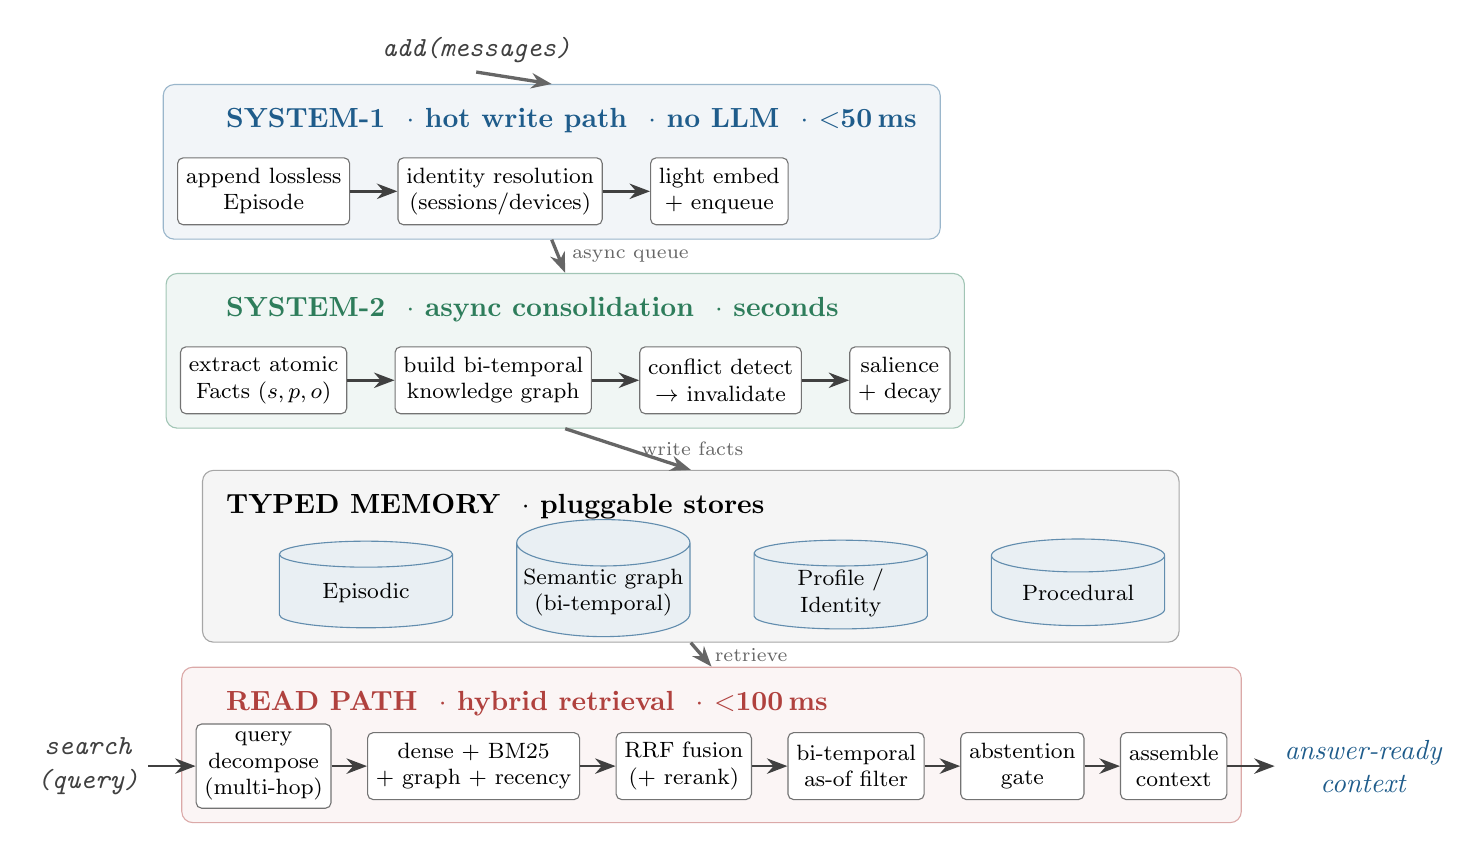
\begin{tikzpicture}[
  font=\footnotesize,
  chip/.style={rounded corners=2pt, draw=black!55, fill=white, inner sep=3pt,
               minimum height=8.5mm, align=center},
  store/.style={cylinder, shape border rotate=90, aspect=0.28, draw=engramblue!70,
                fill=engramblue!10, minimum height=11mm, minimum width=22mm, align=center,
                inner sep=1pt},
  io/.style={font=\itshape, text=black!75, align=center},
  ttl/.style={font=\bfseries, anchor=west},
  >={Stealth[length=2.6mm]},
  flow/.style={->, line width=1pt, draw=black!75},
  vflow/.style={->, line width=1.2pt, draw=black!60},
]
% ----- input -----
\node[io] (in) at (3.0,10.2) {\texttt{add(messages)}};
% ----- SYSTEM-1 -----
\node[ttl, text=engramblue] (t1) at (-0.3,9.3) {SYSTEM-1 \ $\cdot$\ hot write path \ $\cdot$\ no LLM \ $\cdot$\ $<$50\,ms};
\node[chip] (s1a) at (0.3,8.4) {append lossless\\Episode};
\node[chip, right=6mm of s1a] (s1b) {identity resolution\\(sessions/devices)};
\node[chip, right=6mm of s1b] (s1c) {light embed\\$+$ enqueue};
\draw[flow] (s1a)--(s1b); \draw[flow] (s1b)--(s1c);
% ----- SYSTEM-2 -----
\node[ttl, text=s2green] (t2) at (-0.3,6.9) {SYSTEM-2 \ $\cdot$\ async consolidation \ $\cdot$\ seconds};
\node[chip] (s2a) at (0.3,6.0) {extract atomic\\Facts $(s,p,o)$};
\node[chip, right=6mm of s2a] (s2b) {build bi-temporal\\knowledge graph};
\node[chip, right=6mm of s2b] (s2c) {conflict detect\\$\to$ invalidate};
\node[chip, right=6mm of s2c] (s2d) {salience\\$+$ decay};
\draw[flow] (s2a)--(s2b); \draw[flow] (s2b)--(s2c); \draw[flow] (s2c)--(s2d);
% ----- TYPED MEMORY -----
\node[ttl] (t3) at (-0.3,4.4) {TYPED MEMORY \ $\cdot$\ pluggable stores};
\node[store] (m1) at (1.6,3.3) {Episodic};
\node[store, right=8mm of m1] (m2) {Semantic graph\\(bi-temporal)};
\node[store, right=8mm of m2] (m3) {Profile /\\Identity};
\node[store, right=8mm of m3] (m4) {Procedural};
% ----- READ PATH -----
\node[ttl, text=baselinered] (t4) at (-0.3,1.9) {READ PATH \ $\cdot$\ hybrid retrieval \ $\cdot$\ $<$100\,ms};
\node[chip] (r1) at (0.3,1.1) {query\\decompose\\(multi-hop)};
\node[chip, right=4.5mm of r1] (r2) {dense $+$ BM25\\$+$ graph $+$ recency};
\node[chip, right=4.5mm of r2] (r3) {RRF fusion\\($+$ rerank)};
\node[chip, right=4.5mm of r3] (r4) {bi-temporal\\as-of filter};
\node[chip, right=4.5mm of r4] (r5) {abstention\\gate};
\node[chip, right=4.5mm of r5] (r6) {assemble\\context};
\draw[flow] (r1)--(r2); \draw[flow] (r2)--(r3); \draw[flow] (r3)--(r4);
\draw[flow] (r4)--(r5); \draw[flow] (r5)--(r6);
\node[io, left=6mm of r1] (q) {\texttt{search}\\\texttt{(query)}};
\draw[flow] (q)--(r1);
\node[io, right=6mm of r6, text=engramblue] (out) {answer-ready\\context};
\draw[flow] (r6)--(out);
% ----- background bands -----
\begin{scope}[on background layer]
\node[rounded corners=4pt, fill=engramblue!6, draw=engramblue!45, fit=(t1)(s1a)(s1c), inner sep=5pt] (bandS1) {};
\node[rounded corners=4pt, fill=s2green!7, draw=s2green!45, fit=(t2)(s2a)(s2d), inner sep=5pt] (bandS2) {};
\node[rounded corners=4pt, fill=black!4, draw=black!35, fit=(t3)(m1)(m4), inner sep=5pt] (bandM) {};
\node[rounded corners=4pt, fill=baselinered!5, draw=baselinered!45, fit=(t4)(r1)(r6), inner sep=5pt] (bandR) {};
\end{scope}
% ----- vertical flow between bands -----
\draw[vflow] (in.south)--(bandS1.north);
\draw[vflow] (bandS1.south)--node[right=1pt,font=\scriptsize,text=black!60]{async queue}(bandS2.north);
\draw[vflow] (bandS2.south)--node[right=1pt,font=\scriptsize,text=black!60]{write facts}(bandM.north);
\draw[vflow] (bandM.south)--node[right=1pt,font=\scriptsize,text=black!60]{retrieve}(bandR.north);
\end{tikzpicture}%
}
\caption{The \engram{} dual-process architecture: a hot write path (\textsc{System-1}) that never blocks on
an LLM; an asynchronous consolidation path (\textsc{System-2}) that extracts facts, builds the bi-temporal
graph and resolves conflicts non-destructively; a typed memory over pluggable stores; and a hybrid read path
(dense $+$ lexical $+$ graph $+$ recency, fused by RRF) with an as-of filter and an abstention gate.}
\label{fig:arch}
\end{figure}

\subsection{Bi-temporal data model}

Two time axes are first-class everywhere, which is what makes knowledge-updates and ``as-of'' queries
intrinsic rather than bolted-on.

\begin{itemize}
  \item \textbf{Episode} --- a raw, lossless turn/event, stamped with \emph{event time} (when it happened in
  the world) and \emph{ingested-at} (transaction time, when we recorded it).
  \item \textbf{Fact} --- an atomic $(\textit{subject},\textit{predicate},\textit{object})$ claim with surface
  text, an embedding, a \emph{salience} and \emph{confidence}, and \emph{provenance} (the source episode
  ids). It carries two time axes: \emph{valid time} (\texttt{valid\_at} / \texttt{invalid\_at}, when the claim
  is true in the world) and \emph{transaction time} (\texttt{created\_at} / \texttt{expired\_at}, when we
  learned or retracted it), plus a \texttt{supersedes} pointer to the fact it replaces.
  \item \textbf{Entity / Relation} --- graph nodes and edges; edges carry the same bi-temporal stamps.
\end{itemize}

The invariant: \emph{never hard-delete a contradicted fact---invalidate it} (set \texttt{invalid\_at}) and
keep the history. Every fact can therefore answer ``where did this come from?'' and ``what did it replace?''
(Figure~\ref{fig:bitemporal}).

\begin{figure}[t]
\centering
\resizebox{0.8\textwidth}{!}{%
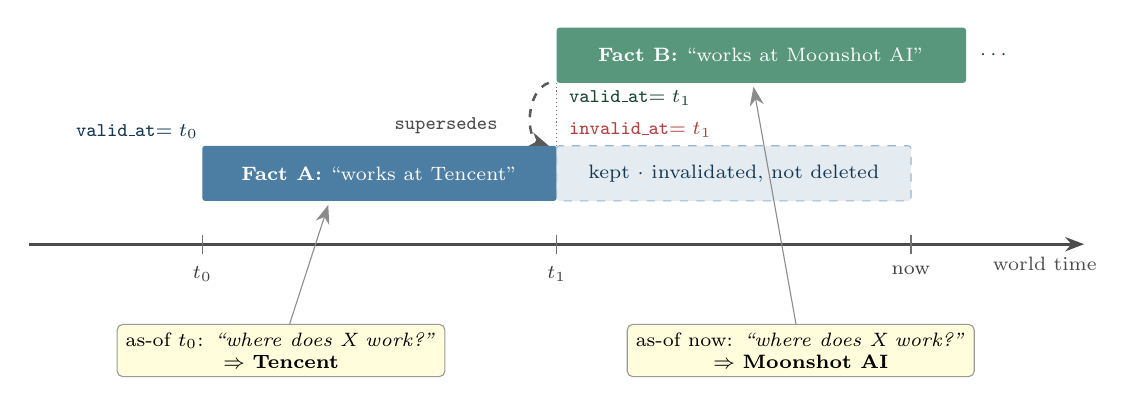
\begin{tikzpicture}[font=\footnotesize, >={Stealth[length=2.4mm]}]
% time axis
\draw[->, line width=1pt, black!70] (-0.2,0)--(13.2,0);
\node[font=\scriptsize, text=black!70, below] at (12.7,-0.04) {world time};
\foreach \x/\lab in {2/{$t_0$}, 6.5/{$t_1$}, 11/{now}}{
  \draw[black!55] (\x,0.12)--(\x,-0.12);
  \node[below, font=\scriptsize, text=black!75] at (\x,-0.16) {\lab};
}
% Fact A: valid in [t0,t1)
\fill[engramblue!80, rounded corners=1pt] (2,0.55) rectangle (6.5,1.25);
\node[white, font=\scriptsize] at (4.25,0.9) {\textbf{Fact A:} ``works at Tencent''};
% Fact A kept-but-invalid in [t1, now]
\draw[fill=engramblue!12, draw=engramblue!45, dashed, rounded corners=1pt] (6.5,0.55) rectangle (11,1.25);
\node[text=engramblue!60!black, font=\scriptsize] at (8.75,0.9) {kept $\cdot$ invalidated, not deleted};
\node[font=\scriptsize, text=engramblue!60!black, above left=-1pt and -2pt] at (2,1.25) {\texttt{valid\_at}$=t_0$};
% Fact B: valid in [t1, ...)
\fill[s2green!80, rounded corners=1pt] (6.5,2.05) rectangle (11.7,2.75);
\node[white, font=\scriptsize] at (9.1,2.4) {\textbf{Fact B:} ``works at Moonshot AI''};
\node[text=s2green!55!black, font=\scriptsize, right] at (11.75,2.4) {$\cdots$};
% supersession instant at t1
\draw[densely dotted, black!55] (6.5,1.25)--(6.5,2.05);
\node[font=\scriptsize, text=baselinered, right=1pt] at (6.5,1.45) {\texttt{invalid\_at}$=t_1$};
\node[font=\scriptsize, text=s2green!55!black, right=1pt] at (6.5,1.86) {\texttt{valid\_at}$=t_1$};
% supersedes arrow B -> A (bowing left of t1)
\draw[->, dashed, line width=0.9pt, black!65] (6.4,2.05) to[out=-160,in=160] (6.4,1.25);
\node[font=\scriptsize, text=black!70, left=5pt] at (6.05,1.5) {\texttt{supersedes}};
% as-of queries
\node[rounded corners=2pt, draw=black!40, fill=yellow!14, font=\scriptsize, align=center, inner sep=3pt]
  (qa) at (3,-1.35) {as-of $t_0$: \emph{``where does X work?''}\\$\Rightarrow$ \textbf{Tencent}};
\node[rounded corners=2pt, draw=black!40, fill=yellow!14, font=\scriptsize, align=center, inner sep=3pt]
  (qb) at (9.6,-1.35) {as-of now: \emph{``where does X work?''}\\$\Rightarrow$ \textbf{Moonshot AI}};
\draw[->, black!45] (qa)--(3.6,0.5);
\draw[->, black!45] (qb)--(9.0,2.0);
\end{tikzpicture}%
}
\caption{Bi-temporal facts make contradictions and ``as-of'' queries first-class: when Fact~B arrives at
$t_1$, \engram{} sets $\text{A.}\texttt{invalid\_at}=t_1$ and $\text{B.}\texttt{supersedes}=\text{A}$---A is
\emph{invalidated, not deleted}, so history and provenance survive---and a point-in-time query resolves
against the fact valid at that time, which is what the knowledge-update and temporal categories require.}
\label{fig:bitemporal}
\end{figure}

\subsection{System-1: the hot write path}

On \texttt{add(messages)}, \engram{} appends a lossless episode, resolves identity (linking a user/entity
across sessions and devices), computes a light embedding, and enqueues the episode for consolidation. No LLM
runs on this path, keeping it within a sub-50ms budget so writes never block the agent.

\subsection{System-2: asynchronous consolidation}

Off the critical path, the consolidation engine (i) extracts atomic facts from episodes (rule-based by
default, LLM-based when a model is configured), (ii) builds the bi-temporal knowledge graph of entities and
relations, (iii) detects conflicts and invalidates superseded facts, and (iv) scores salience and applies
decay/reinforcement so unreinforced memories fade and the store stays small and fast. Hierarchical
abstraction (session summaries $\rightarrow$ profile) runs here as well.

\subsection{Cheap-then-escalate conflict resolution}

When a new fact arrives for an existing $(\textit{subject},\textit{predicate})$ slot with a different object,
\engram{} resolves it in increasing order of cost. First, cheap signals: an exact \textbf{slot match}
signals a likely update, \textbf{embedding similarity} catches the same attribute under a different
free-form predicate, and \textbf{content subsumption} (one claim $\subseteq$ the other) separates
contradiction from elaboration. Second, if the claims are clearly contradictory and temporally ordered, the
old one is invalidated ($\texttt{old.invalid\_at} \leftarrow \texttt{new.valid\_at}$) and
$\texttt{new.supersedes} \leftarrow \texttt{old.id}$---with \emph{no LLM call}. Only genuinely ambiguous cases
escalate to an LLM adjudicator. This is the cost win over systems that invoke an LLM on every fact, while
preserving temporal correctness and a complete audit trail.

\subsection{The hybrid read path}

On \texttt{search(query)}, \engram{} (1) understands the query and, for multi-hop questions, decomposes it
into sub-queries; (2) retrieves in parallel through four complementary channels---dense semantic, BM25
lexical, graph $n$-hop from the query's entities, and recency/salience; (3) fuses the ranked lists with
Reciprocal Rank Fusion~\citep{cormack2009rrf} and an optional cross-encoder rerank over the top-$k$ (off by
default); (4) applies a bi-temporal ``as-of'' filter (what we believed was true at time $T$); (5) passes an
abstention gate that declines to answer when the evidence is absent; and (6) assembles a deduplicated,
provenance-tagged, token-budgeted context. The per-item score combines all signals:
\begin{equation}
\label{eq:score}
\begin{split}
\mathrm{score}(\textit{item} \mid q) ={}&
  w_{\text{sem}}\cos(q,\textit{item})
  + w_{\text{lex}}\,\mathrm{bm25}(q,\textit{item})
  + w_{\text{graph}}\,\mathrm{prox}(\textit{item}) \\
  &{}+ w_{\text{rec}}\,e^{-\Delta t/\tau}
  + w_{\text{sal}}\,\mathrm{sal}(\textit{item}),
\end{split}
\end{equation}
where the weights are configuration-driven and tuned on the harness rather than hand-set. Crucially, the
assembled context is \emph{hybrid}: it contains both the conflict-resolved bi-temporal facts and the most
relevant raw session chunks (plus session-level summaries). \S\ref{sec:results} shows this hybrid composition
is necessary---facts alone lose recall.

Every external dependency---LLM, embedder, vector, graph and lexical store---sits behind an interface with
a zero-dependency offline fallback, so the loop runs with no API keys (Appendix~\ref{app:backends}).

\section{Experimental Setup}
\label{sec:setup}

\paragraph{Benchmark.}
\textsc{LongMemEval}\textsubscript{S}~\citep{wu2025longmemeval}: 500 questions, each over a haystack of
$\sim$50 sessions ($\sim$115k tokens), pulled from the public release. Questions span seven categories
(Figure~\ref{fig:percat}). We grade with the \emph{official} category-specific judge prompts---including the
temporal off-by-one tolerance, knowledge-update old-information tolerance, preference-rubric leniency, the
``contains the answer'' semantics, and unanswerable (abstention) detection---rather than a home-grown judge.

\paragraph{Models.}
Embedder: \texttt{BAAI/bge-small-en-v1.5} (local, no API key). System-2 fact extractor:
\texttt{doubao-seed-1.6-flash}. Answerer: \texttt{doubao-seed-2.0-pro} for the headline, and the small
\texttt{doubao-seed-1.6-flash} as a second backbone (\S\ref{sec:backbones}). Judge: DeepSeek's official API
(\texttt{deepseek-chat}, which served DeepSeek-V4-Flash at the time of the runs), prompted with the official
LongMemEval judge prompts; footnote~\ref{fn:judge} explains why this differs from the arXiv~v1 judge. Models
are addressed as \texttt{provider:model} and resolved via LiteLLM, so any OpenAI-compatible endpoint (OpenAI,
DeepSeek, a local model) can be substituted and the same commands run.

\paragraph{Systems.}
\lean{} (our headline) retrieves a small hybrid slice---conflict-resolved bi-temporal facts $+$ the most
relevant raw session chunks $+$ session summaries---and answers from \emph{that alone} ($\sim$7.9k tokens),
never the full history. \full{} is the baseline: stuff the entire haystack into the prompt ($\sim$79k tokens).
The harness applies the \emph{same answerer and judge to every system}, so any within-run comparison is
apples-to-apples by construction.

\paragraph{Retrieval configuration.}
The hybrid read path fuses five ranked signals by weighted Reciprocal Rank Fusion ($k_{\text{RRF}}=60$) with
the Eq.~\eqref{eq:score} weights $w_{\text{sem}}=1.0$, $w_{\text{lex}}=0.6$, $w_{\text{graph}}=0.8$,
$w_{\text{rec}}=0.3$, $w_{\text{sal}}=0.25$ (the repository defaults in \texttt{engram/config.py}, tuned on
the harness, not hand-set per question). The lean slice assembles up to 8 conflict-resolved facts, the
top-15 fused items, 2 raw session chunks, and 28 session-level summaries; exact flag semantics are in the
reproduce command.

\paragraph{Reproduce.}
The headline run is a single command, given verbatim (with the model identifiers and every flag) in the
Reproducibility Statement; its raw per-question log is committed to the repository as
\texttt{results/run500\_v3\_main\_deepseekjudge.jsonl}. The second backbone swaps the answerer flag and the
LOCOMO slice the data flag, nothing else. \texttt{python eval/report.py <run.jsonl>} recomputes every table
below from a log, and \texttt{python paper/check\_numbers.py} asserts that every number in this paper's
main text equals a value recomputed from the committed logs.

\paragraph{Measurement-integrity notes.}
Six bugs and drifts that silently inflate or deflate memory-benchmark numbers---and that we hit and fixed
ourselves---are documented in Appendix~\ref{app:integrity}: a ``memory'' system that still contained the
full history, a truncated full-context baseline, a home-grown judge stricter than the official one,
abstention grading, retry handling (the headline run has 0 errored questions of 500 under both systems),
and the judge-endpoint drift of footnote~\ref{fn:judge}. They are the reason cross-source numbers disagree.

\section{Results}
\label{sec:results}

\paragraph{Headline.}
Table~\ref{tab:headline} and Figure~\ref{fig:acctokens} report the full 500-question result. \engram{}'s lean
configuration beats the full-context baseline by \textbf{$+5.6$ points} (84.4\% vs.\ 78.8\%) while using
\textbf{10$\times$ fewer tokens} (7.9k vs.\ 79k), with 0 of 500 errored under both. The filtered slice is not
merely cheaper---it is \emph{more accurate} than the full window, consistent with the distractor mechanism
of \citet{liu2024lost}. The margin is statistically significant but not large: across the 500 paired
questions \lean{} is correct on 68 that the baseline misses versus 40 the other way (McNemar's exact test,
$p=0.009$), and a paired bootstrap puts the 95\% CI of the gain at $+1.6$ to $+9.6$ points. All statistics
are recomputed from the committed log by \texttt{paper/compute\_stats.py}.

\begin{table}[h]
\centering
\caption{\textsc{LongMemEval}\textsubscript{S}, 500 questions, official judge prompts; same answerer
(\texttt{doubao-seed-2.0-pro}) and judge (\texttt{deepseek-chat}) for both systems. Accuracy with a Wilson
95\% CI (paired difference: McNemar exact $p=0.009$); latency is end-to-end wall-clock per question
including the remote answerer call, p50\,/\,p95.}
\label{tab:headline}
\resizebox{\linewidth}{!}{%
\begin{tabular}{lcrrr}
\toprule
System & Overall acc.\ (95\% CI) & Avg.\ context tokens & Latency p50\,/\,p95 & Errors \\
\midrule
\textbf{\engram{}} (\lean{}) & \textbf{84.4\%} \,[81.0,\,87.3] & \textbf{7.9k} & 52.9\,s\,/\,118.7\,s & 0 / 500 \\
full-context baseline        & 78.8\% \,[75.0,\,82.2]          & 79.2k         & 14.6\,s\,/\,59.2\,s  & 0 / 500 \\
\bottomrule
\end{tabular}}
\end{table}

\begin{figure}[t]
\centering
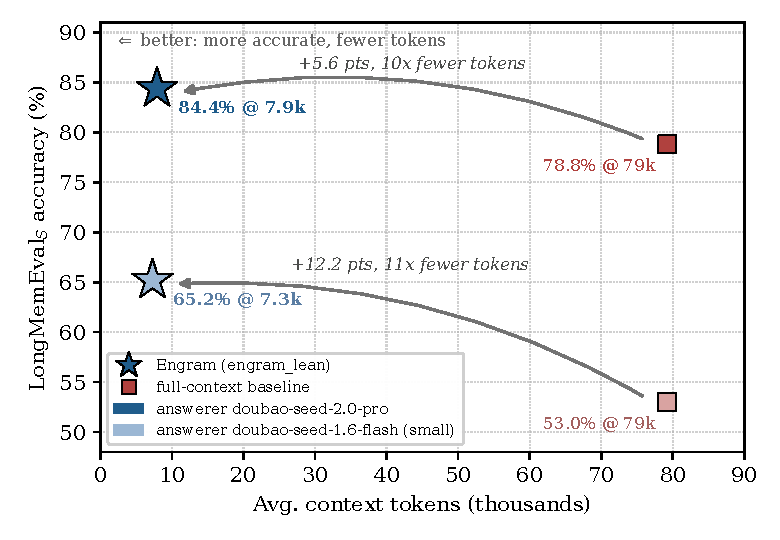
\includegraphics[width=0.62\textwidth]{fig_acc_tokens.pdf}
\caption{Accuracy vs.\ average context tokens on LongMemEval\textsubscript{S} (500 questions) for two answerer
backbones: \lean{} (star) sits up and to the left of full-context (square)---\textbf{$+5.6$ points at
10$\times$ fewer tokens} for \texttt{doubao-seed-2.0-pro}, $+12.2$ at 11$\times$ for the small
\texttt{doubao-seed-1.6-flash} (Table~\ref{tab:backbones}).}
\label{fig:acctokens}
\end{figure}

\paragraph{Per-category.}
Table~\ref{tab:percat} and Figure~\ref{fig:percat} break both systems down by category. The lean slice wins
four of the six categories and ties one. The margins are largest where the full window has the most to
distract from: \emph{single-session-preference} ($+30.0$; a category that is hard field-wide, and where the
baseline reaches only 50.0\%), \emph{multi-session} aggregation ($+11.3$; counting and aggregating across
many sessions, where the baseline mostly abstains) and \emph{single-session-user} ($+8.6$).
\emph{Temporal-reasoning} (date-stamped context $+$ as-of filtering) is a modest $+2.3$. The one loss is
\emph{knowledge-update} ($-6.4$): the baseline sees every version of a changed value in order and applies
``most recent wins'' itself, whereas the lean slice depends on consolidation having attached the update to
the right slot. Of the eight knowledge-update questions the slice loses and the baseline gets, seven end in
a superseded value or an abstention---consistent with the update not reaching the slice, a consolidation
miss rather than a reading error (\S\ref{sec:limitations}). The 30 \emph{abstention} items, graded by the
official \emph{unanswerable} judge and counted inside their host categories above, come out at 90.0\% for
\lean{} vs.\ 93.3\% for the baseline: the abstention gate declines correctly on most of them, at a small
cost against a baseline that, as the error analysis below shows, abstains often anyway.

\begin{table}[h]
\centering\footnotesize
\caption{Per-category accuracy on \textsc{LongMemEval}\textsubscript{S} (500 questions; the run of
Table~\ref{tab:headline}). $\Delta$ is \lean{} minus full-context. The 30 unanswerable (abstention) items are
counted inside their host categories; broken out, they score 90.0\% (\lean{}) vs.\ 93.3\% (full-context).}
\label{tab:percat}
\begin{tabular}{lrrrr}
\toprule
Category & \lean{} & full-context & $\Delta$ & $n$ \\
\midrule
multi-session             & \textbf{78.2\%} & 66.9\%          & $+11.3$ & 133 \\
temporal-reasoning        & \textbf{83.5\%} & 81.2\%          & $+2.3$  & 133 \\
knowledge-update          & 84.6\%          & \textbf{91.0\%} & $-6.4$  & 78 \\
single-session-user       & \textbf{91.4\%} & 82.9\%          & $+8.6$  & 70 \\
single-session-assistant  & 94.6\%          & 94.6\%          & $+0.0$  & 56 \\
single-session-preference & \textbf{80.0\%} & 50.0\%          & $+30.0$ & 30 \\
\midrule
overall                   & \textbf{84.4\%} & 78.8\%          & $+5.6$  & 500 \\
\bottomrule
\end{tabular}
\end{table}

\begin{figure}[t]
\centering
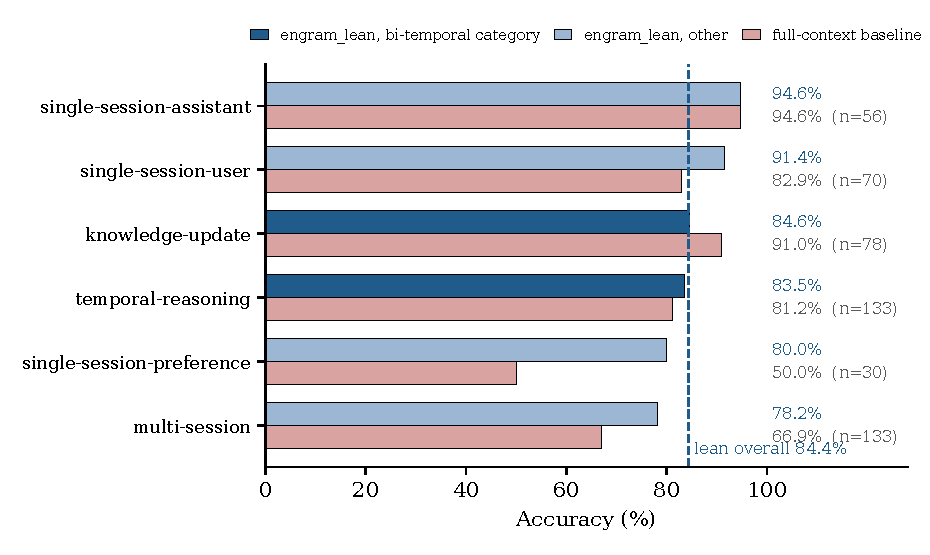
\includegraphics[width=0.74\textwidth]{fig_percat.pdf}
\caption{Per-category accuracy of \lean{} vs.\ full-context on the full 500-question set (dashed line: the
84.4\% lean overall). The two bi-temporal categories are highlighted: temporal-reasoning a small win,
knowledge-update the one loss; the largest margins are single-session-preference and multi-session.}
\label{fig:percat}
\end{figure}

\paragraph{Error analysis: full-context is ``lost in the middle.''}
The two systems fail differently. Of the full-context baseline's 106 errors, \textbf{57\% (60) are
abstentions}---it answers ``I don't know'' even though, by construction, the evidence lies somewhere in its
$\sim$79k-token window; it simply fails to locate it. On the 68 questions where \lean{} is correct and
full-context is wrong, full-context abstains on 59\% (40) and returns a \emph{wrong} value on the other 28.
\lean{}, answering from a $\sim$7.9k-token slice, abstains on 60/500---and 27 of those are among the 30
genuinely unanswerable items. This is the ``lost in the middle'' effect~\citep{liu2024lost} made
quantitative: past a point, more context is \emph{not} more accuracy if the model cannot find the relevant
span (counts recomputed from the committed logs by \texttt{paper/compute\_stats.py}).

\paragraph{The read path must be hybrid.}
A load-bearing finding from development: a \emph{facts-only} read path---answering purely from extracted
$(s,p,o)$ facts---\emph{loses recall} relative to the hybrid path, because extraction drops detail that some
questions need verbatim. Adding the most relevant raw session chunks back alongside the conflict-resolved
facts restores that detail; the facts contribute conflict-resolved, bi-temporal signal and the chunks restore
specificity. The headline configuration is hybrid for exactly this reason, and we caution against shipping
facts-only QA. We report this as a design observation; a controlled facts-only ablation on the full
500-question set under the same judge is reported as future work (\S\ref{sec:limitations}), not claimed here.

\paragraph{Efficiency.}
The retrieved context averages $\sim$7.9k tokens, 10$\times$ leaner than the $\sim$79k full-context
baseline; the saving is in prompt tokens, the quantity that grows with history. End-to-end latency per
question is \emph{higher} for \lean{} (p50 52.9\,s vs.\ 14.6\,s, Table~\ref{tab:headline}). The harness
records wall-clock per question including the remote answerer call and does not instrument retrieval
separately, so we report the latency as measured and make no retrieval-latency claim from these logs.

\subsection{A second backbone: the weaker the reader, the larger the gain}
\label{sec:backbones}

Memory quality should not depend on one model's ability to read our structures, so the same 500 questions
were also run with the answerer swapped for the small \texttt{doubao-seed-1.6-flash}, everything else
unchanged (Table~\ref{tab:backbones}). That run was made in June on the revision of that date and graded by
the judge that has since been retired (footnote~\ref{fn:judge}), so the table names the code revision and
judge per row and we include the June run of the pro answerer as its within-judge sibling; every row is a
within-run, same-judge comparison, which is the claim we make. The lean slice wins under every backbone and
judge, and the margin is \emph{largest for the weakest reader}: $+12.2$ points (65.2\% vs.\ 53.0\%) for the
small answerer, against $+3.0$ for the pro answerer under the same judge and code, and $+5.6$ on the current
code, at a $\sim$10--11$\times$ token ratio throughout. With the small answerer the lean advantage holds in
five of six categories, the exception being single-session-assistant, which is near ceiling for both
(per-category gaps in Appendix~\ref{app:flash}). The reading is simple: a strong model can partly compensate for a
noisy window by searching it; a weak one cannot, so removing distractors is worth more to it. That is the
regime that matters for cheap and local deployments.

\begin{table}[h]
\centering\small
\caption{Answerer backbones on the same 500 questions, extractor and harness (gap $=$ \lean{} $-$
full-context; token ratio $=$ full-context / lean tokens). Each row is a within-run comparison under one
judge; rows differ in code revision and judge as marked, so compare gaps, not levels, across rows. Logs:
\texttt{run500\_v3\_main\_deepseekjudge}, \texttt{headline\_500}, \texttt{bb\_flash} (\texttt{results/*.jsonl}).}
\label{tab:backbones}
\resizebox{\linewidth}{!}{%
\begin{tabular}{llrrrr}
\toprule
Answerer & Code / judge & \lean{} & full-context & Gap & Token ratio \\
\midrule
\texttt{doubao-seed-2.0-pro}   & current / \texttt{deepseek-chat}    & \textbf{84.4\%} & 78.8\% & $+5.6$  & 10.0$\times$ \\
\texttt{doubao-seed-2.0-pro}   & June 2026 / retired ARK judge & \textbf{79.0\%} & 76.0\% & $+3.0$  & 10.9$\times$ \\
\texttt{doubao-seed-1.6-flash} & June 2026 / retired ARK judge & \textbf{65.2\%} & 53.0\% & $+12.2$ & 10.9$\times$ \\
\bottomrule
\end{tabular}}
\end{table}

\subsection{A second benchmark: a 200-item LOCOMO slice}
\label{sec:locomo}

% TODO(locomo-full): the full 1986-item LOCOMO run (results/locomo1986_main_deepseekjudge.jsonl) is in
% flight. When it lands: repoint LOCOMO_SLICE in compute_stats.py, replace the numbers in this subsection
% and in the abstract/related-work mentions, and drop the "slice" labels.
LOCOMO~\citep{maharana2024locomo} is a different regime: ten long multi-session conversations whose full
text is only $\sim$16k tokens, a fraction of a \textsc{LongMemEval}\textsubscript{S} haystack. We converted
its QA pairs into the harness's item format so that the \emph{same} answerer, extractor and judge apply
(its adversarial questions map onto the unanswerable judge), and report the \textbf{first 200 of its 1,986
items}---a slice, labelled as such; the full run is in progress. Table~\ref{tab:locomo} gives the result.
Overall the two systems tie (88.0\% vs.\ 89.0\%, $-1.0$; 0 errors under both) at 3.4k vs.\ 16.2k tokens
($\sim$5$\times$). That the margin shrinks to zero here is the expected behaviour, not a regression: with a
16k-token history there is little for retrieval to remove and the full-context reader is not yet lost. The
lean advantage is a function of how much distracting history there is---clear on the $\sim$79k-token
\textsc{LongMemEval} windows, nil on 16k---and we expect it to grow, not shrink, with history length.

The per-category split carries the information. Two of \engram{}'s design bets get independent evidence:
\emph{adversarial} (the answer is not in the conversation) is 100.0\% vs.\ 91.1\% ($+8.9$, $n=45$)---the
abstention gate declines correctly on every item, where the full-context reader answers some---and
\emph{multi-hop} is 78.6\% vs.\ 71.4\% ($+7.1$, $n=28$), the category the multi-hop query planner targets
and one \textsc{LongMemEval} has no separate label for. Single-hop is within noise ($-3.6$, $n=83$). The
clear loss is \emph{temporal-reasoning} ($-16.2$, $n=37$), and its failures are not retrieval misses but
\emph{date-granularity} errors: gold answers such as ``the week before 9 June 2023'' or ``the first weekend
of August'' come back as a single collapsed timestamp, off by weeks or a month, because fact extraction
reduces a relative time expression to one point on the axis while the full-context reader still sees the
original phrasing. This is a limitation of the current extractor that \textsc{LongMemEval}'s more regular
date annotations did not expose---the concrete value of a second benchmark---and it is the next target for
the bi-temporal model (\S\ref{sec:limitations}).

\begin{table}[h]
\centering\footnotesize
\caption{LOCOMO, first 200 of 1,986 items (a slice; the full run is in progress). Same answerer, extractor
and judge as Table~\ref{tab:headline}; log \texttt{results/locomo200\_main\_deepseekjudge.jsonl}, 0 errors.}
\label{tab:locomo}
\begin{tabular}{lrrrr}
\toprule
Category & \lean{} & full-context & $\Delta$ & $n$ \\
\midrule
single-hop         & 90.4\%           & \textbf{94.0\%} & $-3.6$  & 83 \\
adversarial        & \textbf{100.0\%} & 91.1\%          & $+8.9$  & 45 \\
temporal-reasoning & 78.4\%           & \textbf{94.6\%} & $-16.2$ & 37 \\
multi-hop          & \textbf{78.6\%}  & 71.4\%          & $+7.1$  & 28 \\
open-domain        & \textbf{71.4\%}  & 57.1\%          & $+14.3$ & 7 \\
\midrule
overall            & 88.0\%           & \textbf{89.0\%} & $-1.0$  & 200 \\
avg.\ context tokens & 3.4k           & 16.2k           &         & \\
\bottomrule
\end{tabular}
\end{table}

\section{Discussion and Limitations}
\label{sec:limitations}

Because our thesis is that cross-harness numbers are not comparable, we state the honest scope of the
present evidence rather than a leaderboard ``win'':

\begin{itemize}
  \item \textbf{Two backbones from one family; one full benchmark plus a slice.} The headline is
  \textsc{LongMemEval}\textsubscript{S} with a mid-size and a small answerer from the same model family, and
  the small-answerer run predates the judge migration (\S\ref{sec:backbones}). A frontier-class answerer, a
  re-run of the small answerer under the current judge, and the full 1,986-item LOCOMO set (in progress)
  are the immediate next steps, so that memory quality is shown not to depend on one model's ability to
  read our structures.
  \item \textbf{Where the slice loses.} Knowledge-update on \textsc{LongMemEval} ($-6.4$) and
  temporal-reasoning on LOCOMO ($-16.2$) are the two categories where the full-context reader beats the
  lean slice, and both point at consolidation rather than retrieval: an update the extractor misses leaves a
  stale value in the slice, and a relative time expression collapsed to one timestamp loses the granularity
  the question needs. Fixing extraction, not adding context, is the lever.
  \item \textbf{Small samples mislead.} During development, small slices repeatedly read far above the
  full-set truth; we therefore report \emph{only} full-set numbers on \textsc{LongMemEval}, and label the
  LOCOMO result as a slice.
  \item \textbf{Open categories.} Multi-session aggregation and preference are where headroom remains; the
  multi-hop query planner and tuned bi-temporal conflict resolution are the levers we expect to move them.
  \item \textbf{Single run per configuration; no controlled component ablation yet.} We report one full-set
  run per system and backbone and do not quantify run-to-run variance from answerer stochasticity; the
  paired bootstrap interval ($+1.6$ to $+9.6$) is the honest statement of uncertainty for the headline gap,
  and the full-context baseline's spread across full-set runs under one judge (footnote~\ref{fn:judge})
  suggests that noise band is real. Nor do we report a controlled full-set ablation of the read path's
  components (notably the facts-only vs.\ hybrid comparison of \S\ref{sec:results}, which we state as an
  observation). Both are immediate next work.
\end{itemize}

\section{Conclusion}

\engram{} shows that a precisely retrieved, bi-temporal, hybrid context can beat the full-context baseline
\emph{on accuracy}---$+5.6$ points at 10$\times$ fewer tokens on the full \textsc{LongMemEval}\textsubscript{S}
under the official judge prompts, and $+12.2$ for a small answerer---turning long-term memory from a cost
optimization into a quality improvement. Equally,
we contribute the neutral, reproducible harness that makes such a claim checkable: the official judge baked in,
the full-context baseline in every table, documented measurement-integrity pitfalls, and the raw logs published.
In a field where every number is contested, the trustworthy scoreboard is itself the result. The system, the
harness, and the logs are open source\ifanon{} in a public repository (link withheld for double-blind
review; see the Reproducibility Statement)\else{} at \url{https://github.com/ly-wang19/engram}\fi.

\section*{AI Use Statement}
\label{sec:aiuse}

LLM-based AI coding assistants were used in producing this work, in two ways that we separate explicitly.
First, as engineering tools: they wrote and refactored parts of the \engram{} code base, the evaluation
harness, the statistics and figure scripts, and drafted and edited passages of this manuscript under the
authors' direction. Second, as \emph{measured components}: the answerer, the fact extractor and the judge
are LLMs and are named, with model identifiers, in \S\ref{sec:setup}; they are the object of study, not an
authoring aid. The human authors designed the system and the experiments, ran and checked every run,
verified every number against the committed logs (\texttt{paper/check\_numbers.py}), and take full
responsibility for all claims, text and code in the paper.

\section*{Reproducibility Statement}
\label{sec:repro}

Every number in this paper is produced by the in-repo harness and backed by committed per-question logs
(prediction, gold, correctness, tokens, and latency for every question of every run cited: both answerer
backbones on \textsc{LongMemEval}\textsubscript{S} and the LOCOMO slice), and \texttt{paper/check\_numbers.py}
asserts that every number in the main text equals a value recomputed from those logs. The end-to-end loop and unit
tests run with no API keys and no external services via deterministic offline fallbacks; the benchmark
numbers require an OpenAI-compatible model endpoint for the answerer, extractor, and judge, all configurable.
The model identifiers, embedder, and hyper-parameters are in \S\ref{sec:setup}, and the headline run is
the single command below (log: \texttt{results/run500\_v3\_main\_deepseekjudge.jsonl}):
\begin{list}{}{\leftmargin=1em}\item[]\footnotesize\ttfamily
python eval/bench.py --data s --limit 500 --systems engram\_lean,full\_context \textbackslash\\
\hspace*{1.5em}--answerer volcano:doubao-seed-2-0-pro-260215 --judge deepseek \textbackslash\\
\hspace*{1.5em}--extractor volcano:doubao-seed-1-6-flash-250615 --embedder bge-small \textbackslash\\
\hspace*{1.5em}--reasoning --persona --chunks 2 --topk 15 --extract-k 8 \textbackslash\\
\hspace*{1.5em}--summ-k 28 --n-summaries 28
\end{list}
Substitutions: \texttt{--answerer volcano:doubao-seed-1-6-flash-250615} for the second backbone;
\texttt{--data locomo --limit 200} for the LOCOMO slice (items converted from the public release by
\texttt{eval/locomo.py}). The appendix reproduces every prompt verbatim. The significance tests and
confidence intervals in \S\ref{sec:results} are recomputed from the committed logs by
\texttt{paper/compute\_stats.py}, with no model calls. The code, the harness and the raw logs are
\ifanon in a public repository whose link is withheld for double-blind review and will be given in the
camera-ready version\else at \url{https://github.com/ly-wang19/engram}\fi; the benchmark data
(\textsc{LongMemEval} and LOCOMO) are the public releases.

\section*{Ethics Statement}
\label{sec:ethics}

A long-term memory layer necessarily persists personal data across sessions, which raises real privacy
obligations. Two of \engram{}'s core design choices are mitigations as much as features: \emph{non-destructive
invalidation with full provenance} yields an auditable trail of what was believed, when, and from which
source, and \emph{salience decay} lets unreinforced personal details fade by default. Non-destructive
invalidation is a statement about \emph{contradiction}, not about \emph{erasure}: a contradicted fact is
kept, invalidated, so that the history stays auditable, but the store also exposes explicit deletion---a
single fact, or everything held about a user---so that a ``right to be forgotten'' request is a supported
operation rather than a best-effort one. Because every component has a zero-dependency offline fallback,
\engram{} can run fully locally---no user data need leave the operator's machine---and the AGPL-3.0 license
keeps self-hosted data under the operator's control. The principal risks are the obverse of the benefits: a
memory store concentrates sensitive information and must be secured, access-controlled, and scoped to genuine
consent; and a memory that confidently surfaces a \emph{stale} or \emph{wrong} fact can mislead, which is
precisely why the bi-temporal model and the abstention gate (decline when memory lacks the answer) are
first-class rather than optional. All experiments use the public \textsc{LongMemEval} and LOCOMO releases,
whose conversations are synthetic or already published; no private user data were collected or used.

\bibliographystyle{plainnat}
\bibliography{references}

\appendix
\label{app:start}

\section{Prompts}
\label{app:prompts}

For full reproducibility we reproduce the exact prompts the harness uses, verbatim from the repository
(non-ASCII characters are normalised for typesetting). The \emph{answerer} system prompt (used with
\texttt{--reasoning}; it instructs evidence aggregation, most-recent-wins on conflicts, and abstention
only as a last resort):

\begin{lstlisting}[style=prompt]
You answer the user's question using the provided dated context. The context has two parts: a FACTS
index (a digest) AND the full dated CONVERSATIONS below it. The answer is USUALLY present -- search BOTH
parts thoroughly before concluding anything. The dates are real; use them for temporal reasoning.

DIG FOR THE ANSWER FIRST. Most questions ARE answerable from the history -- your job is to find the
evidence, not to give up. If the FACTS digest doesn't contain it, scan the full CONVERSATIONS below.

WHEN THE QUESTION NEEDS MULTIPLE EVIDENCE PIECES (counting, summing, ordering, date arithmetic, duration,
earliest/latest/most-recent, multi-step lookup, knowledge updated over time):
  EVIDENCE: list EVERY relevant dated item from the context, one per line with its date. Be EXHAUSTIVE
  -- scan the whole history; a missed item makes a count or total wrong. Re-read before finalizing.
  REASON: count distinct items / sum / sort by date / compute the date difference / pick the most recent.
  Show the work in 1-2 lines. For durations compute end_date - start_date explicitly.
  ANSWER: <a single concise final answer -- no reasoning on this line>

FOR DATE/TIME/NUMBER ANSWERS: give the MOST SPECIFIC value the context supports (exact date > month+year
> year; exact duration). Read the exact figure from the text -- don't round (e.g. 27 minutes 45 seconds,
not 28 minutes).

WHEN THE QUESTION ASKS FOR A RECOMMENDATION / PREFERENCE: do NOT refuse, do NOT ask a clarifying question,
do NOT give generic advice. Ground the answer in the user's OWN stated history: name the SPECIFIC people,
places, brands, tools, experiences or constraints they mentioned, and tailor the suggestion to those.

FOR SIMPLE SINGLE-FACT QUESTIONS: go straight to 'ANSWER: <fact>'.

CURRENT-STATE questions ('what is my current/latest X', 'where do I work now'): report ONLY the most
recent value by date and explicitly disregard older, superseded ones. The newest dated statement wins.
When facts conflict, ALWAYS trust the most recent one by date.

ABSTENTION -- a careful LAST resort, only after searching the ENTIRE history (facts AND all conversations)
and the SPECIFIC thing asked is genuinely never stated. Do NOT abstain just because it wasn't in the FACTS
digest. If the question presupposes something the user truly never mentioned, reply exactly 'ANSWER: I
don't know' rather than guessing. Never fabricate a value. The 'ANSWER:' line is REQUIRED.
\end{lstlisting}

\noindent The answer template (the context is the only thing that varies across systems):
\begin{lstlisting}[style=prompt]
Today's date: {qdate}

{context}

Question: {question}
Answer:
\end{lstlisting}

\noindent The System-2 fact-extractor system prompt (a non-English worked example is elided for
typesetting; values are kept in the user's original language, only the predicate is English snake\_case):
\begin{lstlisting}[style=prompt]
You are a precise information-extraction engine for a long-term memory system. From a multi-turn
conversation, extract the atomic, durable facts it states about the user and the people/things they
mention (identities, attributes, preferences, relationships, possessions, goals/plans, and events with
their times). Output ONLY a JSON array of objects, each with keys "subject", "predicate", "object",
"text". Use short snake_case predicates (e.g. works_at, lives_in, favorite_color, owns, married_to,
born_in, visited). Capture PREFERENCES explicitly with predicates like likes, dislikes, prefers, avoids,
allergic_to, favorite_<thing>; for each preference or dislike stated, output a SEPARATE fact. Resolve
first-person ('I','my','me') to the user's name when known, otherwise to "user". Capture a stated name as
{"subject":"user","predicate":"name","object":"<Name>"}. LANGUAGE: keep subject and object VALUES (names,
places, brands, free text) in the SAME language the user used -- do NOT translate them; only the predicate
stays English snake_case. "text" is a natural one-sentence statement in the conversation's language. Do
NOT infer or invent facts that are not stated. If there are no durable facts, output [].
\end{lstlisting}

\noindent We grade with the \emph{official} LongMemEval category-specific judge prompts, reproduced
verbatim so scores are leaderboard-comparable:
\begin{lstlisting}[style=prompt]
[single-session-user / single-session-assistant / multi-session]
I will give you a question, a correct answer, and a response from a model. Please answer yes if the
response contains the correct answer. Otherwise, answer no. If the response is equivalent to the correct
answer or contains all the intermediate steps to get the correct answer, you should also answer yes. If
the response only contains a subset of the information required by the answer, answer no.
Question: {q}   Correct Answer: {a}   Model Response: {r}
Is the model response correct? Answer yes or no only.

[temporal-reasoning]  (as above, plus:)
... do not penalize off-by-one errors for the number of days. If the question asks for the number of
days/weeks/months and the model makes off-by-one errors (e.g., predicting 19 days when the answer is 18),
the model's response is still correct.

[knowledge-update]  (as above, plus:)
... If the response contains some previous information along with an updated answer, the response should
be considered correct as long as the updated answer is the required answer.

[single-session-preference]
I will give you a question, a rubric for desired personalized response, and a response. Answer yes if the
response satisfies the desired response. The model need not reflect all points in the rubric; the response
is correct as long as it recalls and utilizes the user's personal information correctly.

[abstention / unanswerable]
I will give you an unanswerable question, an explanation, and a response. Answer yes if the model correctly
identifies the question as unanswerable (it may say the information is incomplete, or give other
information but not the asked information).
\end{lstlisting}

\section{Measurement-Integrity Notes}
\label{app:integrity}

We document the bugs that silently inflate or deflate memory-benchmark numbers, because they are the reason
cross-source numbers disagree:
\begin{enumerate}
  \item \textbf{Lean, not full-history (the honest test).} An earlier headline prepended facts \emph{above the
  entire history}; because that system \emph{contains} full-context, it cannot really lose to it and does not
  validate the retrieval thesis. The headline is now \lean{}, which answers from a $\sim$7.9k-token retrieved
  slice.
  \item \textbf{Full-context truncation.} The baseline was once capped below the haystack size, feeding it
  only the oldest sessions; this \emph{deflated the baseline}. Fixed so it receives the whole haystack. (Any
  much lower full-context figure from before this fix is a truncation artifact.)
  \item \textbf{Official judge, not a home-grown one.} A generic ``same info?'' judge was \emph{stricter} than
  the official LongMemEval judge and made scores non-comparable; we use the official prompts verbatim.
  \item \textbf{Abstention} questions are graded by the official \emph{unanswerable} judge.
  \item \textbf{Reliability.} The LLM client uses exponential-backoff retry with transient/permanent error
  classification; the headline run completed with \textbf{0 errored questions} of 500 under both systems.
  \item \textbf{Judge endpoint drift.} The judge behind our arXiv~v1 numbers was a third-party endpoint that
  was retired underneath the documented command, and nothing in the repository noticed until the command
  failed; the absolute scores moved when we re-ran under a judge we can still reach
  (footnote~\ref{fn:judge}). A reproducible harness must name its judge beside every number and keep every
  log it cites committed, which is what we now do.
\end{enumerate}

\section{Pluggable Backends}
\label{app:backends}

Every external dependency---LLM, embedder, vector store, graph store, lexical index---sits behind an interface
with a zero-dependency offline fallback (a hashing embedder, a rule-based extractor, in-memory stores). The
end-to-end loop and the unit tests therefore run deterministically with no API keys and no services; real
backends (BGE embeddings, LanceDB/Qdrant/pgvector, Kuzu/Neo4j, any LLM via LiteLLM) slot in behind the same
interfaces.

\section{Second Backbone: Per-Category Gaps}
\label{app:flash}

With the small \texttt{doubao-seed-1.6-flash} answerer (Table~\ref{tab:backbones}; log
\texttt{results/bb\_flash.jsonl}), the lean advantage holds in five of six categories: multi-session
$+16.5$, temporal-reasoning $+15.8$, single-session-user $+12.9$, single-session-preference $+10.0$,
knowledge-update $+9.0$. The exception is single-session-assistant ($-1.8$), which is near ceiling for both
systems. All gaps are \lean{} minus full-context within that run, under its own judge.

\section{Qualitative Examples}
\label{app:examples}

Table~\ref{tab:qual} shows representative cases drawn from the committed headline log
(\texttt{results/run500\_v3\_main\_deepseekjudge.jsonl}) where \lean{} answers correctly and the
full-context baseline does not. Two failure modes recur. \textbf{(i) Lost in the
middle}~\citep{liu2024lost}: the evidence \emph{is} present in full-context's $\sim$79k-token window, yet
it returns ``I don't know,'' while the lean $\sim$7.9k-token slice surfaces it. \textbf{(ii) Wrong value
from a noisy window}: full-context returns a value that is present in the history but is not the one the
question asks for (a stale count, the wrong duration, a neighbouring figure) while the lean slice returns
the current one. These are illustrative, not cherry-picked headline numbers; all per-question records
(prediction, gold, correctness) are in the repository.

\begin{table}[h]
\centering
\footnotesize
\caption{Representative cases from the \textsc{LongMemEval}\textsubscript{S} logs where \lean{} is correct
and full-context is wrong (ID = the benchmark's question id; predictions verbatim, lightly truncated).}
\label{tab:qual}
\begin{tabular}{@{}l p{2.0cm} p{1.9cm} p{2.7cm} p{2.7cm}@{}}
\toprule
ID & Category & Gold & \engram{} (\lean{}) & full-context \\
\midrule
\texttt{69fee5aa} & knowledge-update & 38 & 38 & \emph{37} \\
\texttt{ba61f0b9} & knowledge-update & 6 & 6 & \emph{5} \\
\texttt{0db4c65d} & temporal-reasoning & 18 days & 18 days & \emph{6 days} \\
\texttt{d851d5ba} & multi-session & \$3,750 & \$3750 & \emph{\$8750} \\
\texttt{2311e44b} & multi-session & 190 & 190 pages & \emph{I don't know} \\
\texttt{8ebdbe50} & single-session-user & Data Science & Data Science certification & \emph{I don't know} \\
\bottomrule
\end{tabular}
\end{table}

\end{document}
"  (then bibtex main; pdflatex x2)
\documentclass{article}
\pdfoutput=1 % force pdfLaTeX (the figures are included as PDF)

% Fallback for TeX installs that lack the `helvetic' package: the ICLR style loads Helvetica-Bold (phvb)
% only for the grey reviewer line-number ruler. `texfonts.map' next to this file aliases phvb -> ptmb
% (Times Bold metrics) when phvb.tfm is missing, and this map line gives pdfTeX the matching glyphs.
% On a complete TeX Live the real phvb.tfm is found first and pdfTeX ignores the duplicate map entry.
\pdfmapline{+phvb NimbusRomNo9L-Medi <utmb8a.pfb}

\usepackage{iclr2027/iclr2027_conference,times}
% \iclrfinalcopy is the camera-ready switch: it prints the author block and the "Published as..." header.
% Default is the anonymous submission build; pass \def\FINAL{} on the command line for the named build.
\ifdefined\FINAL\iclrfinalcopy\fi

\usepackage[utf8]{inputenc}
\usepackage[T1]{fontenc}
\usepackage{amsmath,amssymb}
\usepackage{booktabs}
\usepackage{graphicx}
\usepackage{xcolor}
\usepackage{microtype}
\usepackage[colorlinks=true,linkcolor=black,citecolor=blue!50!black,urlcolor=blue!50!black]{hyperref}
\usepackage{url}
\usepackage{tikz}
\usetikzlibrary{arrows.meta,positioning,fit,backgrounds,shapes.geometric,calc}
\graphicspath{{figs/}}
\usepackage{listings}
\lstdefinestyle{prompt}{%
  basicstyle=\ttfamily\scriptsize, breaklines=true, breakautoindent=false,
  columns=fullflexible, keepspaces=true, showstringspaces=false,
  frame=single, framesep=3pt, xleftmargin=3pt, xrightmargin=3pt, aboveskip=5pt, belowskip=5pt}

% ---- shared figure colors / styles ----
\definecolor{engramblue}{HTML}{1F5C8B}
\definecolor{engramlight}{HTML}{9BB7D4}
\definecolor{baselinered}{HTML}{B0413E}
\definecolor{s2green}{HTML}{2E7D5B}

\newcommand{\engram}{\textsc{Engram}}
\newcommand{\lean}{\texttt{engram\_lean}}
\newcommand{\full}{\texttt{full\_context}}

% Anonymity follows the ICLR switch: the submission build (\iclrfinalfalse) carries no author names,
% affiliations, acknowledgements or self-identifying URLs; \ifanon guards every such string in the body.
\newif\ifanon \ificlrfinal\anonfalse\else\anontrue\fi

\title{Less Context, More Accuracy:\\
A Bi-Temporal Memory Engine for LLM Agents\\
Where a Lean Retrieved Context Beats the Full History}

% The style file prints "Anonymous authors / Paper under double-blind review" unless \iclrfinalcopy is
% set, so the block below is typeset only in the camera-ready build.
\ifanon
\author{Anonymous authors}
\else
\author{%
  Liuyin Wang\thanks{Correspondence: \texttt{liuyinwangthu@gmail.com}. Code, raw logs, and the
  reproducible harness: \url{https://github.com/ly-wang19/engram}.}\\
  Independent Researcher%
}
\fi

\begin{document}
\maketitle
% The style sets the running header inside \maketitle's group with fancyhdr's \lhead. The fancyhdr the
% style file bundles (v3.2) makes that global; fancyhdr >= 4 (any current TeX Live) does not, and the
% header vanishes. Re-issue it here, outside the group, with the style's own wording for both builds.
\ificlrfinal\lhead{Published as a conference paper at ICLR 2027}\else\lhead{Under review as a conference paper at ICLR 2027}\fi

\begin{abstract}
Long-term memory is the missing layer for LLM agents: across sessions they forget, and the common
workaround---replaying the entire history into the prompt---is expensive, slow, and, as distractors
accumulate, \emph{less} accurate. Most memory systems win on cost or latency but still lose to the
full-context baseline on accuracy, and the field's benchmark numbers are reported on inconsistent,
non-reproducible harnesses, so the same system appears at wildly different scores across sources.
We present \engram{}, an open-source, dual-process memory engine built on a bi-temporal data model. A fast
write path appends lossless episodes without an LLM on the critical path; an asynchronous consolidation
path extracts atomic $(\textit{subject},\textit{predicate},\textit{object})$ facts, builds a bi-temporal
knowledge graph, and resolves contradictions \emph{without} an LLM call per fact---invalidating, never
deleting, so every fact retains provenance and a supersession chain. A hybrid read path fuses dense, lexical,
graph, and recency/salience signals, applies a point-in-time (``as-of'') temporal filter, and assembles a
compact, provenance-tagged context. On the full 500-question \textsc{LongMemEval}\textsubscript{S} benchmark,
graded with the \emph{official} category-specific judge prompts, \engram{}'s lean configuration---which
answers from a $\sim$7.9k-token retrieved slice, never the full history---scores \textbf{84.4\%} versus
\textbf{78.8\%} for the full-context baseline ($+5.6$ points, McNemar exact $p=0.009$) while using
\textbf{10$\times$ fewer tokens} (7.9k vs.\ 79k), with 0 of 500 questions errored under both systems. The
advantage grows for a weaker reader: with a small answerer the same slice wins by $+12.2$ points. On a
200-item slice of LOCOMO, whose $\sim$16k-token histories leave little for retrieval to remove, the two
tie overall while the lean path wins the adversarial and multi-hop categories. The gain depends on the read
path being \emph{hybrid}: facts alone lose recall; facts plus retrieved raw chunks recover detail. Beyond the
system, we contribute a neutral, in-repo evaluation harness---official judge baked in, full-context baseline
in every table, raw per-question logs published---and document the measurement-integrity pitfalls that
silently distort memory-benchmark numbers. Every number in this paper ships with the command to reproduce it.
\end{abstract}

\section{Introduction}

LLM agents are stateless across sessions. The pragmatic fix---concatenate the whole conversation history into
the prompt---scales badly on three axes at once: token cost grows linearly with history, latency follows, and
accuracy \emph{degrades} as irrelevant turns crowd the window and the model is forced to locate a needle among
distractors~\citep{liu2024lost}. A long-term memory layer that stores, structures, and selectively retrieves
the past is the natural alternative, and a growing body of systems pursues
it~\citep{packer2023memgpt,park2023generative,chhikara2025mem0,rasmussen2025zep,gutierrez2024hipporag};
see \citet{du2026memorysurvey} for a recent (2026) survey.

Two gaps remain wide open. First, \textbf{accuracy}: most memory systems are reported as cheaper or faster
than full-context, but \emph{not more accurate}. Beating full-context \emph{on accuracy}---a precisely
retrieved slice that outperforms the noisy full window---is the harder and more valuable target, because it
turns memory from a cost optimization into a quality improvement. Second, \textbf{reproducibility}: memory
benchmarks are reported on inconsistent harnesses with different ingestion, answer prompts, and judges, so a
single system can appear tens of points apart depending on the source, and different papers give
contradictory orderings. In a field where every number is contested, a neutral harness anyone can re-run is
itself a contribution.

We address both with \engram{}, an open-source memory engine, and its in-repo evaluation harness. Our design
follows a single principle---\emph{a number we cannot reproduce does not exist}---and a composition thesis:
no single mechanism wins, so we compose typed memory, a bi-temporal knowledge graph, multi-signal retrieval
fusion, salience decay, and asynchronous consolidation, and build in the seams between them.

\paragraph{Contributions.}
\begin{enumerate}
  \item \textbf{A dual-process, bi-temporal memory engine} (\S\ref{sec:system}) with cheap, non-destructive
  conflict resolution: a contradicted fact is \emph{invalidated} (with a \texttt{supersedes} chain and full
  provenance), never overwritten, and the common case is resolved with \emph{no} LLM call.
  \item \textbf{The empirical result that a lean retrieved context beats full-context on accuracy}
  (\S\ref{sec:results}): $+5.6$ points (84.4\% vs.\ 78.8\%) at 10$\times$ fewer tokens on the full
  500-question \textsc{LongMemEval}\textsubscript{S} under the official judge prompts\footnote{\label{fn:judge}%
  The arXiv~v1 of this paper reported 83.6\% vs.\ 73.2\% ($+10.4$) at 9.6k vs.\ 79k tokens on the same % arxiv-v1
  500 questions. That run was graded by a DeepSeek-V3.2 judge served through a third-party endpoint that % arxiv-v1
  has since been retired (the model id now returns \texttt{NotFound}), so it can no longer be re-run. % arxiv-v1
  Every number in this version comes from a fresh full-set run of the current code with the judge moved % arxiv-v1
  to DeepSeek's official API (\S\ref{sec:setup}). The judge is what moved the absolute scores: the % arxiv-v1
  unchanged full-context baseline scored 73.2\% and 76.0\% in two full-set runs under the retired judge % arxiv-v1
  and 77.6\%, 77.4\% and 78.8\% in three runs under the current one, while \lean{} moved % arxiv-v1
  83.6\%\,$\rightarrow$\,84.4\%; the gap therefore narrowed from $+10.4$ to $+5.6$. The reproduce % arxiv-v1
  command in \S\ref{sec:setup} targets the current judge; both logs stay committed.}---i.e.\ removing % arxiv-v1
  distractors \emph{raises} accuracy---and the margin widens to $+12.2$ for a small answerer
  (\S\ref{sec:backbones}), together with the finding that a \emph{hybrid} facts-plus-chunks read path is
  load-bearing (facts alone lose recall).
  \item \textbf{A neutral, reproducible harness} (\S\ref{sec:setup}): one in-repo pipeline with the official
  judge baked in, the full-context baseline in every table, the same answerer and judge applied to every
  system by construction, and the raw per-question logs published. We additionally document the
  measurement-integrity pitfalls we found and fixed.
  \item \textbf{A per-category and cross-backbone analysis} (\S\ref{sec:results}) isolating where the lean
  slice wins (multi-session $+11.3$, single-session-preference $+30.0$, single-session-user $+8.6$) and
  where it loses (knowledge-update $-6.4$), plus a second benchmark---a labelled 200-item LOCOMO
  slice (\S\ref{sec:locomo})---that gives independent evidence for the abstention gate and the multi-hop
  planner and exposes a date-granularity limitation of fact extraction.
\end{enumerate}

\section{Related Work}

\paragraph{Memory systems for LLM agents.}
MemGPT~\citep{packer2023memgpt} frames the LLM as an operating system that pages memory in and out of a
limited context window. Generative Agents~\citep{park2023generative} introduce a memory stream with
importance, recency, and relevance scoring plus periodic reflection. Mem0~\citep{chhikara2025mem0} targets
production agents with scalable extract-and-store memory. Zep/Graphiti~\citep{rasmussen2025zep} is the closest
in spirit to \engram{}: a temporally-aware knowledge-graph memory with bi-temporal edges.
HippoRAG~\citep{gutierrez2024hipporag} uses a graph plus personalized PageRank for multi-hop retrieval, and
its successor HippoRAG~2~\citep{gutierrez2025hipporag2} reframes the same machinery as non-parametric continual
memory. The most recent agentic-memory systems add LLM-driven control over how memories are written and
organized: A-MEM~\citep{xu2025amem} builds an interlinked, Zettelkasten-style note network;
MemoryOS~\citep{kang2025memoryos} imposes an operating-system-style short/mid/long-term hierarchy; and
GAM~\citep{wu2026gam} decouples memory encoding from consolidation over hierarchical graphs. \engram{} differs in
\emph{composing} a bi-temporal graph with a hybrid (facts + raw chunks) read path and an explicit, cheap
conflict-resolution policy, and---distinctively---in shipping the neutral harness that lets these design
choices be measured rather than asserted.

\paragraph{Long context and the cost of distractors.}
``Lost in the middle''~\citep{liu2024lost} shows that LLMs use long contexts unevenly and that accuracy
degrades when relevant evidence is buried among distractors. This is the mechanism our headline result
exploits: a filtered, precisely retrieved slice can be \emph{more} accurate than the full window, not merely
cheaper.

\paragraph{Benchmarks.}
\textsc{LongMemEval}~\citep{wu2025longmemeval} evaluates chat assistants on long-term interactive memory
across categories (single/multi-session, knowledge-update, temporal reasoning, preference, and abstention),
with category-specific judge prompts. LOCOMO~\citep{maharana2024locomo} evaluates very long-term
conversational memory, and more recent benchmarks extend the setting to multimodal histories
(Mem-Gallery~\citep{bei2026memgallery}). We report on \textsc{LongMemEval}\textsubscript{S} with two answerer
backbones and on a 200-item LOCOMO slice (\S\ref{sec:locomo}); the full LOCOMO set is in progress
(\S\ref{sec:limitations}).

\paragraph{Retrieval.}
\engram{}'s read path builds on dense retrieval~\citep{karpukhin2020dpr} with modern dense sentence
embeddings (the BGE family~\citep{xiao2024cpack}; we use the English \texttt{bge-small-en-v1.5}), classical
lexical scoring (BM25~\citep{robertson2009bm25}), and Reciprocal Rank Fusion~\citep{cormack2009rrf}, in
the retrieval-augmented generation tradition~\citep{lewis2020rag}. The dual-process framing draws on the System-1/System-2 distinction in
cognitive science~\citep{kahneman2011thinking}, and salience decay on the classical forgetting
curve~\citep{ebbinghaus1913memory}.

\section{The \engram{} System}
\label{sec:system}

\engram{} is a dual-process memory system: a fast online write path (System-1) and a slow asynchronous
consolidation path (System-2) that writes into a typed, bi-temporal memory, which a hybrid read path queries
(Figure~\ref{fig:arch}).

\begin{figure}[t]
\centering
\resizebox{0.84\textwidth}{!}{%
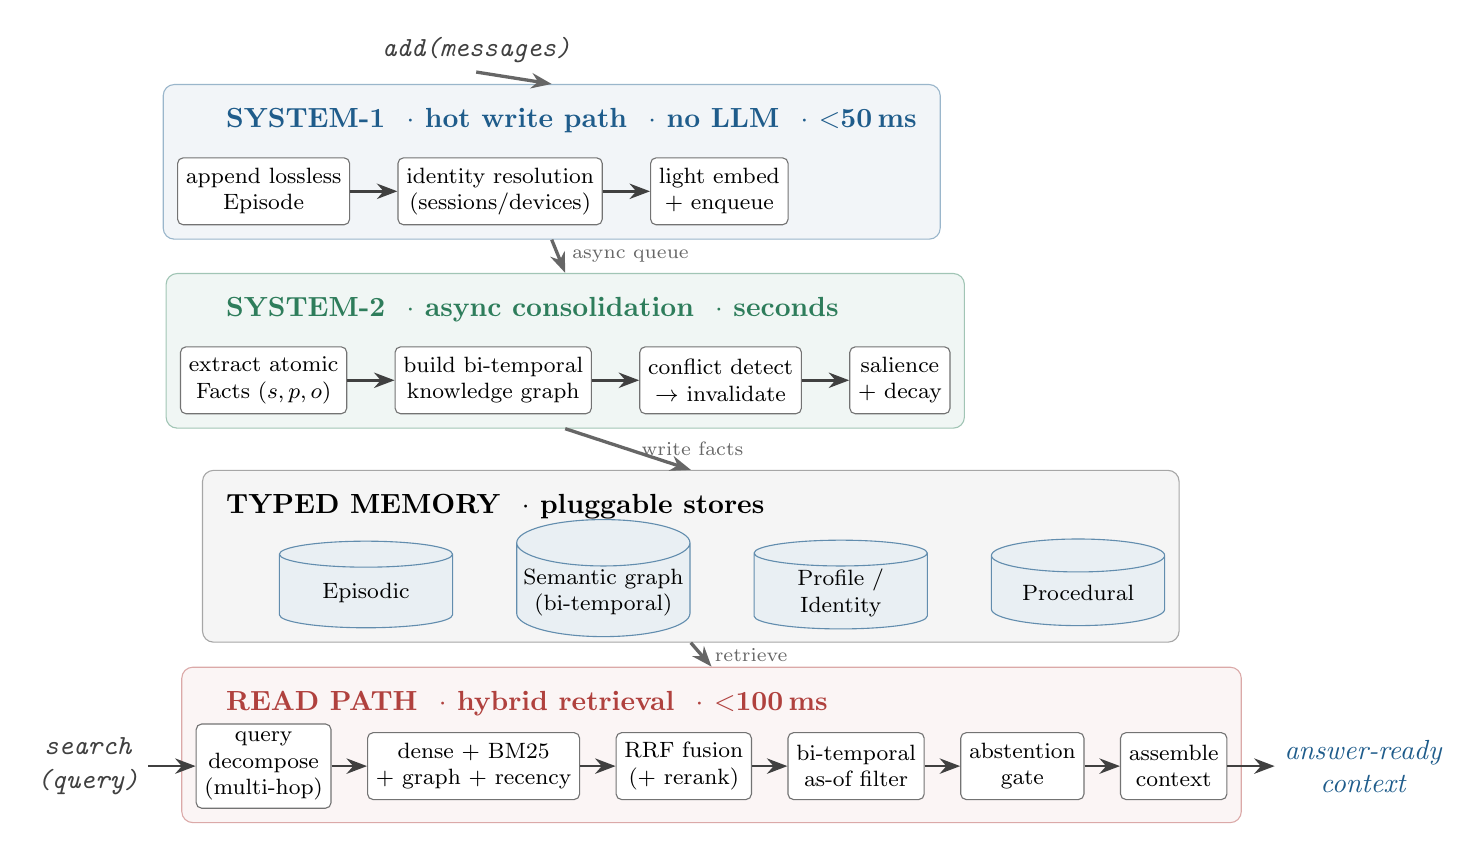
\begin{tikzpicture}[
  font=\footnotesize,
  chip/.style={rounded corners=2pt, draw=black!55, fill=white, inner sep=3pt,
               minimum height=8.5mm, align=center},
  store/.style={cylinder, shape border rotate=90, aspect=0.28, draw=engramblue!70,
                fill=engramblue!10, minimum height=11mm, minimum width=22mm, align=center,
                inner sep=1pt},
  io/.style={font=\itshape, text=black!75, align=center},
  ttl/.style={font=\bfseries, anchor=west},
  >={Stealth[length=2.6mm]},
  flow/.style={->, line width=1pt, draw=black!75},
  vflow/.style={->, line width=1.2pt, draw=black!60},
]
% ----- input -----
\node[io] (in) at (3.0,10.2) {\texttt{add(messages)}};
% ----- SYSTEM-1 -----
\node[ttl, text=engramblue] (t1) at (-0.3,9.3) {SYSTEM-1 \ $\cdot$\ hot write path \ $\cdot$\ no LLM \ $\cdot$\ $<$50\,ms};
\node[chip] (s1a) at (0.3,8.4) {append lossless\\Episode};
\node[chip, right=6mm of s1a] (s1b) {identity resolution\\(sessions/devices)};
\node[chip, right=6mm of s1b] (s1c) {light embed\\$+$ enqueue};
\draw[flow] (s1a)--(s1b); \draw[flow] (s1b)--(s1c);
% ----- SYSTEM-2 -----
\node[ttl, text=s2green] (t2) at (-0.3,6.9) {SYSTEM-2 \ $\cdot$\ async consolidation \ $\cdot$\ seconds};
\node[chip] (s2a) at (0.3,6.0) {extract atomic\\Facts $(s,p,o)$};
\node[chip, right=6mm of s2a] (s2b) {build bi-temporal\\knowledge graph};
\node[chip, right=6mm of s2b] (s2c) {conflict detect\\$\to$ invalidate};
\node[chip, right=6mm of s2c] (s2d) {salience\\$+$ decay};
\draw[flow] (s2a)--(s2b); \draw[flow] (s2b)--(s2c); \draw[flow] (s2c)--(s2d);
% ----- TYPED MEMORY -----
\node[ttl] (t3) at (-0.3,4.4) {TYPED MEMORY \ $\cdot$\ pluggable stores};
\node[store] (m1) at (1.6,3.3) {Episodic};
\node[store, right=8mm of m1] (m2) {Semantic graph\\(bi-temporal)};
\node[store, right=8mm of m2] (m3) {Profile /\\Identity};
\node[store, right=8mm of m3] (m4) {Procedural};
% ----- READ PATH -----
\node[ttl, text=baselinered] (t4) at (-0.3,1.9) {READ PATH \ $\cdot$\ hybrid retrieval \ $\cdot$\ $<$100\,ms};
\node[chip] (r1) at (0.3,1.1) {query\\decompose\\(multi-hop)};
\node[chip, right=4.5mm of r1] (r2) {dense $+$ BM25\\$+$ graph $+$ recency};
\node[chip, right=4.5mm of r2] (r3) {RRF fusion\\($+$ rerank)};
\node[chip, right=4.5mm of r3] (r4) {bi-temporal\\as-of filter};
\node[chip, right=4.5mm of r4] (r5) {abstention\\gate};
\node[chip, right=4.5mm of r5] (r6) {assemble\\context};
\draw[flow] (r1)--(r2); \draw[flow] (r2)--(r3); \draw[flow] (r3)--(r4);
\draw[flow] (r4)--(r5); \draw[flow] (r5)--(r6);
\node[io, left=6mm of r1] (q) {\texttt{search}\\\texttt{(query)}};
\draw[flow] (q)--(r1);
\node[io, right=6mm of r6, text=engramblue] (out) {answer-ready\\context};
\draw[flow] (r6)--(out);
% ----- background bands -----
\begin{scope}[on background layer]
\node[rounded corners=4pt, fill=engramblue!6, draw=engramblue!45, fit=(t1)(s1a)(s1c), inner sep=5pt] (bandS1) {};
\node[rounded corners=4pt, fill=s2green!7, draw=s2green!45, fit=(t2)(s2a)(s2d), inner sep=5pt] (bandS2) {};
\node[rounded corners=4pt, fill=black!4, draw=black!35, fit=(t3)(m1)(m4), inner sep=5pt] (bandM) {};
\node[rounded corners=4pt, fill=baselinered!5, draw=baselinered!45, fit=(t4)(r1)(r6), inner sep=5pt] (bandR) {};
\end{scope}
% ----- vertical flow between bands -----
\draw[vflow] (in.south)--(bandS1.north);
\draw[vflow] (bandS1.south)--node[right=1pt,font=\scriptsize,text=black!60]{async queue}(bandS2.north);
\draw[vflow] (bandS2.south)--node[right=1pt,font=\scriptsize,text=black!60]{write facts}(bandM.north);
\draw[vflow] (bandM.south)--node[right=1pt,font=\scriptsize,text=black!60]{retrieve}(bandR.north);
\end{tikzpicture}%
}
\caption{The \engram{} dual-process architecture: a hot write path (\textsc{System-1}) that never blocks on
an LLM; an asynchronous consolidation path (\textsc{System-2}) that extracts facts, builds the bi-temporal
graph and resolves conflicts non-destructively; a typed memory over pluggable stores; and a hybrid read path
(dense $+$ lexical $+$ graph $+$ recency, fused by RRF) with an as-of filter and an abstention gate.}
\label{fig:arch}
\end{figure}

\subsection{Bi-temporal data model}

Two time axes are first-class everywhere, which is what makes knowledge-updates and ``as-of'' queries
intrinsic rather than bolted-on.

\begin{itemize}
  \item \textbf{Episode} --- a raw, lossless turn/event, stamped with \emph{event time} (when it happened in
  the world) and \emph{ingested-at} (transaction time, when we recorded it).
  \item \textbf{Fact} --- an atomic $(\textit{subject},\textit{predicate},\textit{object})$ claim with surface
  text, an embedding, a \emph{salience} and \emph{confidence}, and \emph{provenance} (the source episode
  ids). It carries two time axes: \emph{valid time} (\texttt{valid\_at} / \texttt{invalid\_at}, when the claim
  is true in the world) and \emph{transaction time} (\texttt{created\_at} / \texttt{expired\_at}, when we
  learned or retracted it), plus a \texttt{supersedes} pointer to the fact it replaces.
  \item \textbf{Entity / Relation} --- graph nodes and edges; edges carry the same bi-temporal stamps.
\end{itemize}

The invariant: \emph{never hard-delete a contradicted fact---invalidate it} (set \texttt{invalid\_at}) and
keep the history. Every fact can therefore answer ``where did this come from?'' and ``what did it replace?''
(Figure~\ref{fig:bitemporal}).

\begin{figure}[t]
\centering
\resizebox{0.8\textwidth}{!}{%
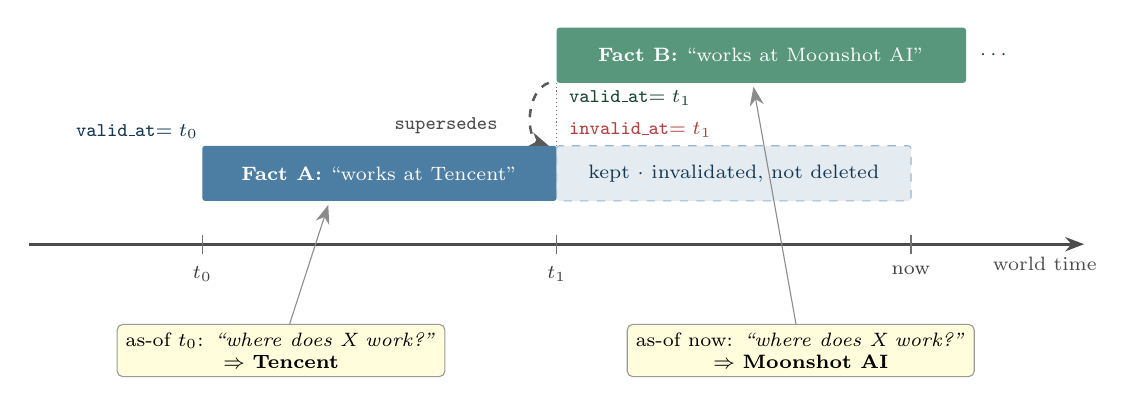
\begin{tikzpicture}[font=\footnotesize, >={Stealth[length=2.4mm]}]
% time axis
\draw[->, line width=1pt, black!70] (-0.2,0)--(13.2,0);
\node[font=\scriptsize, text=black!70, below] at (12.7,-0.04) {world time};
\foreach \x/\lab in {2/{$t_0$}, 6.5/{$t_1$}, 11/{now}}{
  \draw[black!55] (\x,0.12)--(\x,-0.12);
  \node[below, font=\scriptsize, text=black!75] at (\x,-0.16) {\lab};
}
% Fact A: valid in [t0,t1)
\fill[engramblue!80, rounded corners=1pt] (2,0.55) rectangle (6.5,1.25);
\node[white, font=\scriptsize] at (4.25,0.9) {\textbf{Fact A:} ``works at Tencent''};
% Fact A kept-but-invalid in [t1, now]
\draw[fill=engramblue!12, draw=engramblue!45, dashed, rounded corners=1pt] (6.5,0.55) rectangle (11,1.25);
\node[text=engramblue!60!black, font=\scriptsize] at (8.75,0.9) {kept $\cdot$ invalidated, not deleted};
\node[font=\scriptsize, text=engramblue!60!black, above left=-1pt and -2pt] at (2,1.25) {\texttt{valid\_at}$=t_0$};
% Fact B: valid in [t1, ...)
\fill[s2green!80, rounded corners=1pt] (6.5,2.05) rectangle (11.7,2.75);
\node[white, font=\scriptsize] at (9.1,2.4) {\textbf{Fact B:} ``works at Moonshot AI''};
\node[text=s2green!55!black, font=\scriptsize, right] at (11.75,2.4) {$\cdots$};
% supersession instant at t1
\draw[densely dotted, black!55] (6.5,1.25)--(6.5,2.05);
\node[font=\scriptsize, text=baselinered, right=1pt] at (6.5,1.45) {\texttt{invalid\_at}$=t_1$};
\node[font=\scriptsize, text=s2green!55!black, right=1pt] at (6.5,1.86) {\texttt{valid\_at}$=t_1$};
% supersedes arrow B -> A (bowing left of t1)
\draw[->, dashed, line width=0.9pt, black!65] (6.4,2.05) to[out=-160,in=160] (6.4,1.25);
\node[font=\scriptsize, text=black!70, left=5pt] at (6.05,1.5) {\texttt{supersedes}};
% as-of queries
\node[rounded corners=2pt, draw=black!40, fill=yellow!14, font=\scriptsize, align=center, inner sep=3pt]
  (qa) at (3,-1.35) {as-of $t_0$: \emph{``where does X work?''}\\$\Rightarrow$ \textbf{Tencent}};
\node[rounded corners=2pt, draw=black!40, fill=yellow!14, font=\scriptsize, align=center, inner sep=3pt]
  (qb) at (9.6,-1.35) {as-of now: \emph{``where does X work?''}\\$\Rightarrow$ \textbf{Moonshot AI}};
\draw[->, black!45] (qa)--(3.6,0.5);
\draw[->, black!45] (qb)--(9.0,2.0);
\end{tikzpicture}%
}
\caption{Bi-temporal facts make contradictions and ``as-of'' queries first-class: when Fact~B arrives at
$t_1$, \engram{} sets $\text{A.}\texttt{invalid\_at}=t_1$ and $\text{B.}\texttt{supersedes}=\text{A}$---A is
\emph{invalidated, not deleted}, so history and provenance survive---and a point-in-time query resolves
against the fact valid at that time, which is what the knowledge-update and temporal categories require.}
\label{fig:bitemporal}
\end{figure}

\subsection{System-1: the hot write path}

On \texttt{add(messages)}, \engram{} appends a lossless episode, resolves identity (linking a user/entity
across sessions and devices), computes a light embedding, and enqueues the episode for consolidation. No LLM
runs on this path, keeping it within a sub-50ms budget so writes never block the agent.

\subsection{System-2: asynchronous consolidation}

Off the critical path, the consolidation engine (i) extracts atomic facts from episodes (rule-based by
default, LLM-based when a model is configured), (ii) builds the bi-temporal knowledge graph of entities and
relations, (iii) detects conflicts and invalidates superseded facts, and (iv) scores salience and applies
decay/reinforcement so unreinforced memories fade and the store stays small and fast. Hierarchical
abstraction (session summaries $\rightarrow$ profile) runs here as well.

\subsection{Cheap-then-escalate conflict resolution}

When a new fact arrives for an existing $(\textit{subject},\textit{predicate})$ slot with a different object,
\engram{} resolves it in increasing order of cost. First, cheap signals: an exact \textbf{slot match}
signals a likely update, \textbf{embedding similarity} catches the same attribute under a different
free-form predicate, and \textbf{content subsumption} (one claim $\subseteq$ the other) separates
contradiction from elaboration. Second, if the claims are clearly contradictory and temporally ordered, the
old one is invalidated ($\texttt{old.invalid\_at} \leftarrow \texttt{new.valid\_at}$) and
$\texttt{new.supersedes} \leftarrow \texttt{old.id}$---with \emph{no LLM call}. Only genuinely ambiguous cases
escalate to an LLM adjudicator. This is the cost win over systems that invoke an LLM on every fact, while
preserving temporal correctness and a complete audit trail.

\subsection{The hybrid read path}

On \texttt{search(query)}, \engram{} (1) understands the query and, for multi-hop questions, decomposes it
into sub-queries; (2) retrieves in parallel through four complementary channels---dense semantic, BM25
lexical, graph $n$-hop from the query's entities, and recency/salience; (3) fuses the ranked lists with
Reciprocal Rank Fusion~\citep{cormack2009rrf} and an optional cross-encoder rerank over the top-$k$ (off by
default); (4) applies a bi-temporal ``as-of'' filter (what we believed was true at time $T$); (5) passes an
abstention gate that declines to answer when the evidence is absent; and (6) assembles a deduplicated,
provenance-tagged, token-budgeted context. The per-item score combines all signals:
\begin{equation}
\label{eq:score}
\begin{split}
\mathrm{score}(\textit{item} \mid q) ={}&
  w_{\text{sem}}\cos(q,\textit{item})
  + w_{\text{lex}}\,\mathrm{bm25}(q,\textit{item})
  + w_{\text{graph}}\,\mathrm{prox}(\textit{item}) \\
  &{}+ w_{\text{rec}}\,e^{-\Delta t/\tau}
  + w_{\text{sal}}\,\mathrm{sal}(\textit{item}),
\end{split}
\end{equation}
where the weights are configuration-driven and tuned on the harness rather than hand-set. Crucially, the
assembled context is \emph{hybrid}: it contains both the conflict-resolved bi-temporal facts and the most
relevant raw session chunks (plus session-level summaries). \S\ref{sec:results} shows this hybrid composition
is necessary---facts alone lose recall.

Every external dependency---LLM, embedder, vector, graph and lexical store---sits behind an interface with
a zero-dependency offline fallback, so the loop runs with no API keys (Appendix~\ref{app:backends}).

\section{Experimental Setup}
\label{sec:setup}

\paragraph{Benchmark.}
\textsc{LongMemEval}\textsubscript{S}~\citep{wu2025longmemeval}: 500 questions, each over a haystack of
$\sim$50 sessions ($\sim$115k tokens), pulled from the public release. Questions span seven categories
(Figure~\ref{fig:percat}). We grade with the \emph{official} category-specific judge prompts---including the
temporal off-by-one tolerance, knowledge-update old-information tolerance, preference-rubric leniency, the
``contains the answer'' semantics, and unanswerable (abstention) detection---rather than a home-grown judge.

\paragraph{Models.}
Embedder: \texttt{BAAI/bge-small-en-v1.5} (local, no API key). System-2 fact extractor:
\texttt{doubao-seed-1.6-flash}. Answerer: \texttt{doubao-seed-2.0-pro} for the headline, and the small
\texttt{doubao-seed-1.6-flash} as a second backbone (\S\ref{sec:backbones}). Judge: DeepSeek's official API
(\texttt{deepseek-chat}, which served DeepSeek-V4-Flash at the time of the runs), prompted with the official
LongMemEval judge prompts; footnote~\ref{fn:judge} explains why this differs from the arXiv~v1 judge. Models
are addressed as \texttt{provider:model} and resolved via LiteLLM, so any OpenAI-compatible endpoint (OpenAI,
DeepSeek, a local model) can be substituted and the same commands run.

\paragraph{Systems.}
\lean{} (our headline) retrieves a small hybrid slice---conflict-resolved bi-temporal facts $+$ the most
relevant raw session chunks $+$ session summaries---and answers from \emph{that alone} ($\sim$7.9k tokens),
never the full history. \full{} is the baseline: stuff the entire haystack into the prompt ($\sim$79k tokens).
The harness applies the \emph{same answerer and judge to every system}, so any within-run comparison is
apples-to-apples by construction.

\paragraph{Retrieval configuration.}
The hybrid read path fuses five ranked signals by weighted Reciprocal Rank Fusion ($k_{\text{RRF}}=60$) with
the Eq.~\eqref{eq:score} weights $w_{\text{sem}}=1.0$, $w_{\text{lex}}=0.6$, $w_{\text{graph}}=0.8$,
$w_{\text{rec}}=0.3$, $w_{\text{sal}}=0.25$ (the repository defaults in \texttt{engram/config.py}, tuned on
the harness, not hand-set per question). The lean slice assembles up to 8 conflict-resolved facts, the
top-15 fused items, 2 raw session chunks, and 28 session-level summaries; exact flag semantics are in the
reproduce command.

\paragraph{Reproduce.}
The headline run is a single command, given verbatim (with the model identifiers and every flag) in the
Reproducibility Statement; its raw per-question log is committed to the repository as
\texttt{results/run500\_v3\_main\_deepseekjudge.jsonl}. The second backbone swaps the answerer flag and the
LOCOMO slice the data flag, nothing else. \texttt{python eval/report.py <run.jsonl>} recomputes every table
below from a log, and \texttt{python paper/check\_numbers.py} asserts that every number in this paper's
main text equals a value recomputed from the committed logs.

\paragraph{Measurement-integrity notes.}
Six bugs and drifts that silently inflate or deflate memory-benchmark numbers---and that we hit and fixed
ourselves---are documented in Appendix~\ref{app:integrity}: a ``memory'' system that still contained the
full history, a truncated full-context baseline, a home-grown judge stricter than the official one,
abstention grading, retry handling (the headline run has 0 errored questions of 500 under both systems),
and the judge-endpoint drift of footnote~\ref{fn:judge}. They are the reason cross-source numbers disagree.

\section{Results}
\label{sec:results}

\paragraph{Headline.}
Table~\ref{tab:headline} and Figure~\ref{fig:acctokens} report the full 500-question result. \engram{}'s lean
configuration beats the full-context baseline by \textbf{$+5.6$ points} (84.4\% vs.\ 78.8\%) while using
\textbf{10$\times$ fewer tokens} (7.9k vs.\ 79k), with 0 of 500 errored under both. The filtered slice is not
merely cheaper---it is \emph{more accurate} than the full window, consistent with the distractor mechanism
of \citet{liu2024lost}. The margin is statistically significant but not large: across the 500 paired
questions \lean{} is correct on 68 that the baseline misses versus 40 the other way (McNemar's exact test,
$p=0.009$), and a paired bootstrap puts the 95\% CI of the gain at $+1.6$ to $+9.6$ points. All statistics
are recomputed from the committed log by \texttt{paper/compute\_stats.py}.

\begin{table}[h]
\centering
\caption{\textsc{LongMemEval}\textsubscript{S}, 500 questions, official judge prompts; same answerer
(\texttt{doubao-seed-2.0-pro}) and judge (\texttt{deepseek-chat}) for both systems. Accuracy with a Wilson
95\% CI (paired difference: McNemar exact $p=0.009$); latency is end-to-end wall-clock per question
including the remote answerer call, p50\,/\,p95.}
\label{tab:headline}
\resizebox{\linewidth}{!}{%
\begin{tabular}{lcrrr}
\toprule
System & Overall acc.\ (95\% CI) & Avg.\ context tokens & Latency p50\,/\,p95 & Errors \\
\midrule
\textbf{\engram{}} (\lean{}) & \textbf{84.4\%} \,[81.0,\,87.3] & \textbf{7.9k} & 52.9\,s\,/\,118.7\,s & 0 / 500 \\
full-context baseline        & 78.8\% \,[75.0,\,82.2]          & 79.2k         & 14.6\,s\,/\,59.2\,s  & 0 / 500 \\
\bottomrule
\end{tabular}}
\end{table}

\begin{figure}[t]
\centering
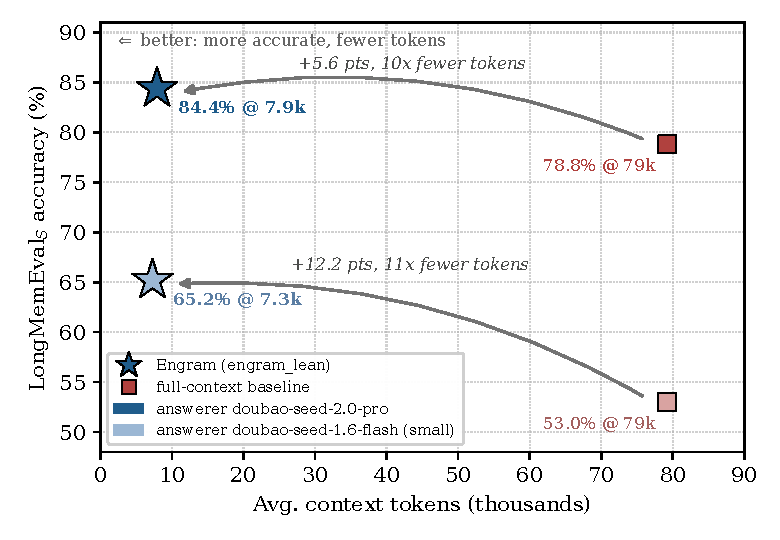
\includegraphics[width=0.62\textwidth]{fig_acc_tokens.pdf}
\caption{Accuracy vs.\ average context tokens on LongMemEval\textsubscript{S} (500 questions) for two answerer
backbones: \lean{} (star) sits up and to the left of full-context (square)---\textbf{$+5.6$ points at
10$\times$ fewer tokens} for \texttt{doubao-seed-2.0-pro}, $+12.2$ at 11$\times$ for the small
\texttt{doubao-seed-1.6-flash} (Table~\ref{tab:backbones}).}
\label{fig:acctokens}
\end{figure}

\paragraph{Per-category.}
Table~\ref{tab:percat} and Figure~\ref{fig:percat} break both systems down by category. The lean slice wins
four of the six categories and ties one. The margins are largest where the full window has the most to
distract from: \emph{single-session-preference} ($+30.0$; a category that is hard field-wide, and where the
baseline reaches only 50.0\%), \emph{multi-session} aggregation ($+11.3$; counting and aggregating across
many sessions, where the baseline mostly abstains) and \emph{single-session-user} ($+8.6$).
\emph{Temporal-reasoning} (date-stamped context $+$ as-of filtering) is a modest $+2.3$. The one loss is
\emph{knowledge-update} ($-6.4$): the baseline sees every version of a changed value in order and applies
``most recent wins'' itself, whereas the lean slice depends on consolidation having attached the update to
the right slot. Of the eight knowledge-update questions the slice loses and the baseline gets, seven end in
a superseded value or an abstention---consistent with the update not reaching the slice, a consolidation
miss rather than a reading error (\S\ref{sec:limitations}). The 30 \emph{abstention} items, graded by the
official \emph{unanswerable} judge and counted inside their host categories above, come out at 90.0\% for
\lean{} vs.\ 93.3\% for the baseline: the abstention gate declines correctly on most of them, at a small
cost against a baseline that, as the error analysis below shows, abstains often anyway.

\begin{table}[h]
\centering\footnotesize
\caption{Per-category accuracy on \textsc{LongMemEval}\textsubscript{S} (500 questions; the run of
Table~\ref{tab:headline}). $\Delta$ is \lean{} minus full-context. The 30 unanswerable (abstention) items are
counted inside their host categories; broken out, they score 90.0\% (\lean{}) vs.\ 93.3\% (full-context).}
\label{tab:percat}
\begin{tabular}{lrrrr}
\toprule
Category & \lean{} & full-context & $\Delta$ & $n$ \\
\midrule
multi-session             & \textbf{78.2\%} & 66.9\%          & $+11.3$ & 133 \\
temporal-reasoning        & \textbf{83.5\%} & 81.2\%          & $+2.3$  & 133 \\
knowledge-update          & 84.6\%          & \textbf{91.0\%} & $-6.4$  & 78 \\
single-session-user       & \textbf{91.4\%} & 82.9\%          & $+8.6$  & 70 \\
single-session-assistant  & 94.6\%          & 94.6\%          & $+0.0$  & 56 \\
single-session-preference & \textbf{80.0\%} & 50.0\%          & $+30.0$ & 30 \\
\midrule
overall                   & \textbf{84.4\%} & 78.8\%          & $+5.6$  & 500 \\
\bottomrule
\end{tabular}
\end{table}

\begin{figure}[t]
\centering
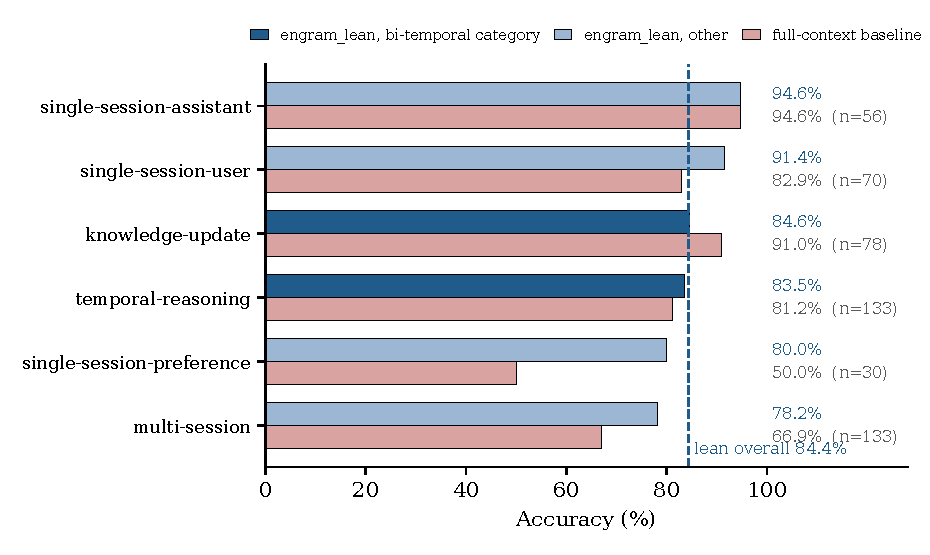
\includegraphics[width=0.74\textwidth]{fig_percat.pdf}
\caption{Per-category accuracy of \lean{} vs.\ full-context on the full 500-question set (dashed line: the
84.4\% lean overall). The two bi-temporal categories are highlighted: temporal-reasoning a small win,
knowledge-update the one loss; the largest margins are single-session-preference and multi-session.}
\label{fig:percat}
\end{figure}

\paragraph{Error analysis: full-context is ``lost in the middle.''}
The two systems fail differently. Of the full-context baseline's 106 errors, \textbf{57\% (60) are
abstentions}---it answers ``I don't know'' even though, by construction, the evidence lies somewhere in its
$\sim$79k-token window; it simply fails to locate it. On the 68 questions where \lean{} is correct and
full-context is wrong, full-context abstains on 59\% (40) and returns a \emph{wrong} value on the other 28.
\lean{}, answering from a $\sim$7.9k-token slice, abstains on 60/500---and 27 of those are among the 30
genuinely unanswerable items. This is the ``lost in the middle'' effect~\citep{liu2024lost} made
quantitative: past a point, more context is \emph{not} more accuracy if the model cannot find the relevant
span (counts recomputed from the committed logs by \texttt{paper/compute\_stats.py}).

\paragraph{The read path must be hybrid.}
A load-bearing finding from development: a \emph{facts-only} read path---answering purely from extracted
$(s,p,o)$ facts---\emph{loses recall} relative to the hybrid path, because extraction drops detail that some
questions need verbatim. Adding the most relevant raw session chunks back alongside the conflict-resolved
facts restores that detail; the facts contribute conflict-resolved, bi-temporal signal and the chunks restore
specificity. The headline configuration is hybrid for exactly this reason, and we caution against shipping
facts-only QA. We report this as a design observation; a controlled facts-only ablation on the full
500-question set under the same judge is reported as future work (\S\ref{sec:limitations}), not claimed here.

\paragraph{Efficiency.}
The retrieved context averages $\sim$7.9k tokens, 10$\times$ leaner than the $\sim$79k full-context
baseline; the saving is in prompt tokens, the quantity that grows with history. End-to-end latency per
question is \emph{higher} for \lean{} (p50 52.9\,s vs.\ 14.6\,s, Table~\ref{tab:headline}). The harness
records wall-clock per question including the remote answerer call and does not instrument retrieval
separately, so we report the latency as measured and make no retrieval-latency claim from these logs.

\subsection{A second backbone: the weaker the reader, the larger the gain}
\label{sec:backbones}

Memory quality should not depend on one model's ability to read our structures, so the same 500 questions
were also run with the answerer swapped for the small \texttt{doubao-seed-1.6-flash}, everything else
unchanged (Table~\ref{tab:backbones}). That run was made in June on the revision of that date and graded by
the judge that has since been retired (footnote~\ref{fn:judge}), so the table names the code revision and
judge per row and we include the June run of the pro answerer as its within-judge sibling; every row is a
within-run, same-judge comparison, which is the claim we make. The lean slice wins under every backbone and
judge, and the margin is \emph{largest for the weakest reader}: $+12.2$ points (65.2\% vs.\ 53.0\%) for the
small answerer, against $+3.0$ for the pro answerer under the same judge and code, and $+5.6$ on the current
code, at a $\sim$10--11$\times$ token ratio throughout. With the small answerer the lean advantage holds in
five of six categories, the exception being single-session-assistant, which is near ceiling for both
(per-category gaps in Appendix~\ref{app:flash}). The reading is simple: a strong model can partly compensate for a
noisy window by searching it; a weak one cannot, so removing distractors is worth more to it. That is the
regime that matters for cheap and local deployments.

\begin{table}[h]
\centering\small
\caption{Answerer backbones on the same 500 questions, extractor and harness (gap $=$ \lean{} $-$
full-context; token ratio $=$ full-context / lean tokens). Each row is a within-run comparison under one
judge; rows differ in code revision and judge as marked, so compare gaps, not levels, across rows. Logs:
\texttt{run500\_v3\_main\_deepseekjudge}, \texttt{headline\_500}, \texttt{bb\_flash} (\texttt{results/*.jsonl}).}
\label{tab:backbones}
\resizebox{\linewidth}{!}{%
\begin{tabular}{llrrrr}
\toprule
Answerer & Code / judge & \lean{} & full-context & Gap & Token ratio \\
\midrule
\texttt{doubao-seed-2.0-pro}   & current / \texttt{deepseek-chat}    & \textbf{84.4\%} & 78.8\% & $+5.6$  & 10.0$\times$ \\
\texttt{doubao-seed-2.0-pro}   & June 2026 / retired ARK judge & \textbf{79.0\%} & 76.0\% & $+3.0$  & 10.9$\times$ \\
\texttt{doubao-seed-1.6-flash} & June 2026 / retired ARK judge & \textbf{65.2\%} & 53.0\% & $+12.2$ & 10.9$\times$ \\
\bottomrule
\end{tabular}}
\end{table}

\subsection{A second benchmark: a 200-item LOCOMO slice}
\label{sec:locomo}

% TODO(locomo-full): the full 1986-item LOCOMO run (results/locomo1986_main_deepseekjudge.jsonl) is in
% flight. When it lands: repoint LOCOMO_SLICE in compute_stats.py, replace the numbers in this subsection
% and in the abstract/related-work mentions, and drop the "slice" labels.
LOCOMO~\citep{maharana2024locomo} is a different regime: ten long multi-session conversations whose full
text is only $\sim$16k tokens, a fraction of a \textsc{LongMemEval}\textsubscript{S} haystack. We converted
its QA pairs into the harness's item format so that the \emph{same} answerer, extractor and judge apply
(its adversarial questions map onto the unanswerable judge), and report the \textbf{first 200 of its 1,986
items}---a slice, labelled as such; the full run is in progress. Table~\ref{tab:locomo} gives the result.
Overall the two systems tie (88.0\% vs.\ 89.0\%, $-1.0$; 0 errors under both) at 3.4k vs.\ 16.2k tokens
($\sim$5$\times$). That the margin shrinks to zero here is the expected behaviour, not a regression: with a
16k-token history there is little for retrieval to remove and the full-context reader is not yet lost. The
lean advantage is a function of how much distracting history there is---clear on the $\sim$79k-token
\textsc{LongMemEval} windows, nil on 16k---and we expect it to grow, not shrink, with history length.

The per-category split carries the information. Two of \engram{}'s design bets get independent evidence:
\emph{adversarial} (the answer is not in the conversation) is 100.0\% vs.\ 91.1\% ($+8.9$, $n=45$)---the
abstention gate declines correctly on every item, where the full-context reader answers some---and
\emph{multi-hop} is 78.6\% vs.\ 71.4\% ($+7.1$, $n=28$), the category the multi-hop query planner targets
and one \textsc{LongMemEval} has no separate label for. Single-hop is within noise ($-3.6$, $n=83$). The
clear loss is \emph{temporal-reasoning} ($-16.2$, $n=37$), and its failures are not retrieval misses but
\emph{date-granularity} errors: gold answers such as ``the week before 9 June 2023'' or ``the first weekend
of August'' come back as a single collapsed timestamp, off by weeks or a month, because fact extraction
reduces a relative time expression to one point on the axis while the full-context reader still sees the
original phrasing. This is a limitation of the current extractor that \textsc{LongMemEval}'s more regular
date annotations did not expose---the concrete value of a second benchmark---and it is the next target for
the bi-temporal model (\S\ref{sec:limitations}).

\begin{table}[h]
\centering\footnotesize
\caption{LOCOMO, first 200 of 1,986 items (a slice; the full run is in progress). Same answerer, extractor
and judge as Table~\ref{tab:headline}; log \texttt{results/locomo200\_main\_deepseekjudge.jsonl}, 0 errors.}
\label{tab:locomo}
\begin{tabular}{lrrrr}
\toprule
Category & \lean{} & full-context & $\Delta$ & $n$ \\
\midrule
single-hop         & 90.4\%           & \textbf{94.0\%} & $-3.6$  & 83 \\
adversarial        & \textbf{100.0\%} & 91.1\%          & $+8.9$  & 45 \\
temporal-reasoning & 78.4\%           & \textbf{94.6\%} & $-16.2$ & 37 \\
multi-hop          & \textbf{78.6\%}  & 71.4\%          & $+7.1$  & 28 \\
open-domain        & \textbf{71.4\%}  & 57.1\%          & $+14.3$ & 7 \\
\midrule
overall            & 88.0\%           & \textbf{89.0\%} & $-1.0$  & 200 \\
avg.\ context tokens & 3.4k           & 16.2k           &         & \\
\bottomrule
\end{tabular}
\end{table}

\section{Discussion and Limitations}
\label{sec:limitations}

Because our thesis is that cross-harness numbers are not comparable, we state the honest scope of the
present evidence rather than a leaderboard ``win'':

\begin{itemize}
  \item \textbf{Two backbones from one family; one full benchmark plus a slice.} The headline is
  \textsc{LongMemEval}\textsubscript{S} with a mid-size and a small answerer from the same model family, and
  the small-answerer run predates the judge migration (\S\ref{sec:backbones}). A frontier-class answerer, a
  re-run of the small answerer under the current judge, and the full 1,986-item LOCOMO set (in progress)
  are the immediate next steps, so that memory quality is shown not to depend on one model's ability to
  read our structures.
  \item \textbf{Where the slice loses.} Knowledge-update on \textsc{LongMemEval} ($-6.4$) and
  temporal-reasoning on LOCOMO ($-16.2$) are the two categories where the full-context reader beats the
  lean slice, and both point at consolidation rather than retrieval: an update the extractor misses leaves a
  stale value in the slice, and a relative time expression collapsed to one timestamp loses the granularity
  the question needs. Fixing extraction, not adding context, is the lever.
  \item \textbf{Small samples mislead.} During development, small slices repeatedly read far above the
  full-set truth; we therefore report \emph{only} full-set numbers on \textsc{LongMemEval}, and label the
  LOCOMO result as a slice.
  \item \textbf{Open categories.} Multi-session aggregation and preference are where headroom remains; the
  multi-hop query planner and tuned bi-temporal conflict resolution are the levers we expect to move them.
  \item \textbf{Single run per configuration; no controlled component ablation yet.} We report one full-set
  run per system and backbone and do not quantify run-to-run variance from answerer stochasticity; the
  paired bootstrap interval ($+1.6$ to $+9.6$) is the honest statement of uncertainty for the headline gap,
  and the full-context baseline's spread across full-set runs under one judge (footnote~\ref{fn:judge})
  suggests that noise band is real. Nor do we report a controlled full-set ablation of the read path's
  components (notably the facts-only vs.\ hybrid comparison of \S\ref{sec:results}, which we state as an
  observation). Both are immediate next work.
\end{itemize}

\section{Conclusion}

\engram{} shows that a precisely retrieved, bi-temporal, hybrid context can beat the full-context baseline
\emph{on accuracy}---$+5.6$ points at 10$\times$ fewer tokens on the full \textsc{LongMemEval}\textsubscript{S}
under the official judge prompts, and $+12.2$ for a small answerer---turning long-term memory from a cost
optimization into a quality improvement. Equally,
we contribute the neutral, reproducible harness that makes such a claim checkable: the official judge baked in,
the full-context baseline in every table, documented measurement-integrity pitfalls, and the raw logs published.
In a field where every number is contested, the trustworthy scoreboard is itself the result. The system, the
harness, and the logs are open source\ifanon{} in a public repository (link withheld for double-blind
review; see the Reproducibility Statement)\else{} at \url{https://github.com/ly-wang19/engram}\fi.

\section*{AI Use Statement}
\label{sec:aiuse}

LLM-based AI coding assistants were used in producing this work, in two ways that we separate explicitly.
First, as engineering tools: they wrote and refactored parts of the \engram{} code base, the evaluation
harness, the statistics and figure scripts, and drafted and edited passages of this manuscript under the
authors' direction. Second, as \emph{measured components}: the answerer, the fact extractor and the judge
are LLMs and are named, with model identifiers, in \S\ref{sec:setup}; they are the object of study, not an
authoring aid. The human authors designed the system and the experiments, ran and checked every run,
verified every number against the committed logs (\texttt{paper/check\_numbers.py}), and take full
responsibility for all claims, text and code in the paper.

\section*{Reproducibility Statement}
\label{sec:repro}

Every number in this paper is produced by the in-repo harness and backed by committed per-question logs
(prediction, gold, correctness, tokens, and latency for every question of every run cited: both answerer
backbones on \textsc{LongMemEval}\textsubscript{S} and the LOCOMO slice), and \texttt{paper/check\_numbers.py}
asserts that every number in the main text equals a value recomputed from those logs. The end-to-end loop and unit
tests run with no API keys and no external services via deterministic offline fallbacks; the benchmark
numbers require an OpenAI-compatible model endpoint for the answerer, extractor, and judge, all configurable.
The model identifiers, embedder, and hyper-parameters are in \S\ref{sec:setup}, and the headline run is
the single command below (log: \texttt{results/run500\_v3\_main\_deepseekjudge.jsonl}):
\begin{list}{}{\leftmargin=1em}\item[]\footnotesize\ttfamily
python eval/bench.py --data s --limit 500 --systems engram\_lean,full\_context \textbackslash\\
\hspace*{1.5em}--answerer volcano:doubao-seed-2-0-pro-260215 --judge deepseek \textbackslash\\
\hspace*{1.5em}--extractor volcano:doubao-seed-1-6-flash-250615 --embedder bge-small \textbackslash\\
\hspace*{1.5em}--reasoning --persona --chunks 2 --topk 15 --extract-k 8 \textbackslash\\
\hspace*{1.5em}--summ-k 28 --n-summaries 28
\end{list}
Substitutions: \texttt{--answerer volcano:doubao-seed-1-6-flash-250615} for the second backbone;
\texttt{--data locomo --limit 200} for the LOCOMO slice (items converted from the public release by
\texttt{eval/locomo.py}). The appendix reproduces every prompt verbatim. The significance tests and
confidence intervals in \S\ref{sec:results} are recomputed from the committed logs by
\texttt{paper/compute\_stats.py}, with no model calls. The code, the harness and the raw logs are
\ifanon in a public repository whose link is withheld for double-blind review and will be given in the
camera-ready version\else at \url{https://github.com/ly-wang19/engram}\fi; the benchmark data
(\textsc{LongMemEval} and LOCOMO) are the public releases.

\section*{Ethics Statement}
\label{sec:ethics}

A long-term memory layer necessarily persists personal data across sessions, which raises real privacy
obligations. Two of \engram{}'s core design choices are mitigations as much as features: \emph{non-destructive
invalidation with full provenance} yields an auditable trail of what was believed, when, and from which
source, and \emph{salience decay} lets unreinforced personal details fade by default. Non-destructive
invalidation is a statement about \emph{contradiction}, not about \emph{erasure}: a contradicted fact is
kept, invalidated, so that the history stays auditable, but the store also exposes explicit deletion---a
single fact, or everything held about a user---so that a ``right to be forgotten'' request is a supported
operation rather than a best-effort one. Because every component has a zero-dependency offline fallback,
\engram{} can run fully locally---no user data need leave the operator's machine---and the AGPL-3.0 license
keeps self-hosted data under the operator's control. The principal risks are the obverse of the benefits: a
memory store concentrates sensitive information and must be secured, access-controlled, and scoped to genuine
consent; and a memory that confidently surfaces a \emph{stale} or \emph{wrong} fact can mislead, which is
precisely why the bi-temporal model and the abstention gate (decline when memory lacks the answer) are
first-class rather than optional. All experiments use the public \textsc{LongMemEval} and LOCOMO releases,
whose conversations are synthetic or already published; no private user data were collected or used.

\bibliographystyle{plainnat}
\bibliography{references}

\appendix
\label{app:start}

\section{Prompts}
\label{app:prompts}

For full reproducibility we reproduce the exact prompts the harness uses, verbatim from the repository
(non-ASCII characters are normalised for typesetting). The \emph{answerer} system prompt (used with
\texttt{--reasoning}; it instructs evidence aggregation, most-recent-wins on conflicts, and abstention
only as a last resort):

\begin{lstlisting}[style=prompt]
You answer the user's question using the provided dated context. The context has two parts: a FACTS
index (a digest) AND the full dated CONVERSATIONS below it. The answer is USUALLY present -- search BOTH
parts thoroughly before concluding anything. The dates are real; use them for temporal reasoning.

DIG FOR THE ANSWER FIRST. Most questions ARE answerable from the history -- your job is to find the
evidence, not to give up. If the FACTS digest doesn't contain it, scan the full CONVERSATIONS below.

WHEN THE QUESTION NEEDS MULTIPLE EVIDENCE PIECES (counting, summing, ordering, date arithmetic, duration,
earliest/latest/most-recent, multi-step lookup, knowledge updated over time):
  EVIDENCE: list EVERY relevant dated item from the context, one per line with its date. Be EXHAUSTIVE
  -- scan the whole history; a missed item makes a count or total wrong. Re-read before finalizing.
  REASON: count distinct items / sum / sort by date / compute the date difference / pick the most recent.
  Show the work in 1-2 lines. For durations compute end_date - start_date explicitly.
  ANSWER: <a single concise final answer -- no reasoning on this line>

FOR DATE/TIME/NUMBER ANSWERS: give the MOST SPECIFIC value the context supports (exact date > month+year
> year; exact duration). Read the exact figure from the text -- don't round (e.g. 27 minutes 45 seconds,
not 28 minutes).

WHEN THE QUESTION ASKS FOR A RECOMMENDATION / PREFERENCE: do NOT refuse, do NOT ask a clarifying question,
do NOT give generic advice. Ground the answer in the user's OWN stated history: name the SPECIFIC people,
places, brands, tools, experiences or constraints they mentioned, and tailor the suggestion to those.

FOR SIMPLE SINGLE-FACT QUESTIONS: go straight to 'ANSWER: <fact>'.

CURRENT-STATE questions ('what is my current/latest X', 'where do I work now'): report ONLY the most
recent value by date and explicitly disregard older, superseded ones. The newest dated statement wins.
When facts conflict, ALWAYS trust the most recent one by date.

ABSTENTION -- a careful LAST resort, only after searching the ENTIRE history (facts AND all conversations)
and the SPECIFIC thing asked is genuinely never stated. Do NOT abstain just because it wasn't in the FACTS
digest. If the question presupposes something the user truly never mentioned, reply exactly 'ANSWER: I
don't know' rather than guessing. Never fabricate a value. The 'ANSWER:' line is REQUIRED.
\end{lstlisting}

\noindent The answer template (the context is the only thing that varies across systems):
\begin{lstlisting}[style=prompt]
Today's date: {qdate}

{context}

Question: {question}
Answer:
\end{lstlisting}

\noindent The System-2 fact-extractor system prompt (a non-English worked example is elided for
typesetting; values are kept in the user's original language, only the predicate is English snake\_case):
\begin{lstlisting}[style=prompt]
You are a precise information-extraction engine for a long-term memory system. From a multi-turn
conversation, extract the atomic, durable facts it states about the user and the people/things they
mention (identities, attributes, preferences, relationships, possessions, goals/plans, and events with
their times). Output ONLY a JSON array of objects, each with keys "subject", "predicate", "object",
"text". Use short snake_case predicates (e.g. works_at, lives_in, favorite_color, owns, married_to,
born_in, visited). Capture PREFERENCES explicitly with predicates like likes, dislikes, prefers, avoids,
allergic_to, favorite_<thing>; for each preference or dislike stated, output a SEPARATE fact. Resolve
first-person ('I','my','me') to the user's name when known, otherwise to "user". Capture a stated name as
{"subject":"user","predicate":"name","object":"<Name>"}. LANGUAGE: keep subject and object VALUES (names,
places, brands, free text) in the SAME language the user used -- do NOT translate them; only the predicate
stays English snake_case. "text" is a natural one-sentence statement in the conversation's language. Do
NOT infer or invent facts that are not stated. If there are no durable facts, output [].
\end{lstlisting}

\noindent We grade with the \emph{official} LongMemEval category-specific judge prompts, reproduced
verbatim so scores are leaderboard-comparable:
\begin{lstlisting}[style=prompt]
[single-session-user / single-session-assistant / multi-session]
I will give you a question, a correct answer, and a response from a model. Please answer yes if the
response contains the correct answer. Otherwise, answer no. If the response is equivalent to the correct
answer or contains all the intermediate steps to get the correct answer, you should also answer yes. If
the response only contains a subset of the information required by the answer, answer no.
Question: {q}   Correct Answer: {a}   Model Response: {r}
Is the model response correct? Answer yes or no only.

[temporal-reasoning]  (as above, plus:)
... do not penalize off-by-one errors for the number of days. If the question asks for the number of
days/weeks/months and the model makes off-by-one errors (e.g., predicting 19 days when the answer is 18),
the model's response is still correct.

[knowledge-update]  (as above, plus:)
... If the response contains some previous information along with an updated answer, the response should
be considered correct as long as the updated answer is the required answer.

[single-session-preference]
I will give you a question, a rubric for desired personalized response, and a response. Answer yes if the
response satisfies the desired response. The model need not reflect all points in the rubric; the response
is correct as long as it recalls and utilizes the user's personal information correctly.

[abstention / unanswerable]
I will give you an unanswerable question, an explanation, and a response. Answer yes if the model correctly
identifies the question as unanswerable (it may say the information is incomplete, or give other
information but not the asked information).
\end{lstlisting}

\section{Measurement-Integrity Notes}
\label{app:integrity}

We document the bugs that silently inflate or deflate memory-benchmark numbers, because they are the reason
cross-source numbers disagree:
\begin{enumerate}
  \item \textbf{Lean, not full-history (the honest test).} An earlier headline prepended facts \emph{above the
  entire history}; because that system \emph{contains} full-context, it cannot really lose to it and does not
  validate the retrieval thesis. The headline is now \lean{}, which answers from a $\sim$7.9k-token retrieved
  slice.
  \item \textbf{Full-context truncation.} The baseline was once capped below the haystack size, feeding it
  only the oldest sessions; this \emph{deflated the baseline}. Fixed so it receives the whole haystack. (Any
  much lower full-context figure from before this fix is a truncation artifact.)
  \item \textbf{Official judge, not a home-grown one.} A generic ``same info?'' judge was \emph{stricter} than
  the official LongMemEval judge and made scores non-comparable; we use the official prompts verbatim.
  \item \textbf{Abstention} questions are graded by the official \emph{unanswerable} judge.
  \item \textbf{Reliability.} The LLM client uses exponential-backoff retry with transient/permanent error
  classification; the headline run completed with \textbf{0 errored questions} of 500 under both systems.
  \item \textbf{Judge endpoint drift.} The judge behind our arXiv~v1 numbers was a third-party endpoint that
  was retired underneath the documented command, and nothing in the repository noticed until the command
  failed; the absolute scores moved when we re-ran under a judge we can still reach
  (footnote~\ref{fn:judge}). A reproducible harness must name its judge beside every number and keep every
  log it cites committed, which is what we now do.
\end{enumerate}

\section{Pluggable Backends}
\label{app:backends}

Every external dependency---LLM, embedder, vector store, graph store, lexical index---sits behind an interface
with a zero-dependency offline fallback (a hashing embedder, a rule-based extractor, in-memory stores). The
end-to-end loop and the unit tests therefore run deterministically with no API keys and no services; real
backends (BGE embeddings, LanceDB/Qdrant/pgvector, Kuzu/Neo4j, any LLM via LiteLLM) slot in behind the same
interfaces.

\section{Second Backbone: Per-Category Gaps}
\label{app:flash}

With the small \texttt{doubao-seed-1.6-flash} answerer (Table~\ref{tab:backbones}; log
\texttt{results/bb\_flash.jsonl}), the lean advantage holds in five of six categories: multi-session
$+16.5$, temporal-reasoning $+15.8$, single-session-user $+12.9$, single-session-preference $+10.0$,
knowledge-update $+9.0$. The exception is single-session-assistant ($-1.8$), which is near ceiling for both
systems. All gaps are \lean{} minus full-context within that run, under its own judge.

\section{Qualitative Examples}
\label{app:examples}

Table~\ref{tab:qual} shows representative cases drawn from the committed headline log
(\texttt{results/run500\_v3\_main\_deepseekjudge.jsonl}) where \lean{} answers correctly and the
full-context baseline does not. Two failure modes recur. \textbf{(i) Lost in the
middle}~\citep{liu2024lost}: the evidence \emph{is} present in full-context's $\sim$79k-token window, yet
it returns ``I don't know,'' while the lean $\sim$7.9k-token slice surfaces it. \textbf{(ii) Wrong value
from a noisy window}: full-context returns a value that is present in the history but is not the one the
question asks for (a stale count, the wrong duration, a neighbouring figure) while the lean slice returns
the current one. These are illustrative, not cherry-picked headline numbers; all per-question records
(prediction, gold, correctness) are in the repository.

\begin{table}[h]
\centering
\footnotesize
\caption{Representative cases from the \textsc{LongMemEval}\textsubscript{S} logs where \lean{} is correct
and full-context is wrong (ID = the benchmark's question id; predictions verbatim, lightly truncated).}
\label{tab:qual}
\begin{tabular}{@{}l p{2.0cm} p{1.9cm} p{2.7cm} p{2.7cm}@{}}
\toprule
ID & Category & Gold & \engram{} (\lean{}) & full-context \\
\midrule
\texttt{69fee5aa} & knowledge-update & 38 & 38 & \emph{37} \\
\texttt{ba61f0b9} & knowledge-update & 6 & 6 & \emph{5} \\
\texttt{0db4c65d} & temporal-reasoning & 18 days & 18 days & \emph{6 days} \\
\texttt{d851d5ba} & multi-session & \$3,750 & \$3750 & \emph{\$8750} \\
\texttt{2311e44b} & multi-session & 190 & 190 pages & \emph{I don't know} \\
\texttt{8ebdbe50} & single-session-user & Data Science & Data Science certification & \emph{I don't know} \\
\bottomrule
\end{tabular}
\end{table}

\end{document}
"  (then bibtex main; pdflatex x2)
\documentclass{article}
\pdfoutput=1 % force pdfLaTeX (the figures are included as PDF)

% Fallback for TeX installs that lack the `helvetic' package: the ICLR style loads Helvetica-Bold (phvb)
% only for the grey reviewer line-number ruler. `texfonts.map' next to this file aliases phvb -> ptmb
% (Times Bold metrics) when phvb.tfm is missing, and this map line gives pdfTeX the matching glyphs.
% On a complete TeX Live the real phvb.tfm is found first and pdfTeX ignores the duplicate map entry.
\pdfmapline{+phvb NimbusRomNo9L-Medi <utmb8a.pfb}

\usepackage{iclr2027/iclr2027_conference,times}
% \iclrfinalcopy is the camera-ready switch: it prints the author block and the "Published as..." header.
% Default is the anonymous submission build; pass \def\FINAL{} on the command line for the named build.
\ifdefined\FINAL\iclrfinalcopy\fi

\usepackage[utf8]{inputenc}
\usepackage[T1]{fontenc}
\usepackage{amsmath,amssymb}
\usepackage{booktabs}
\usepackage{graphicx}
\usepackage{xcolor}
\usepackage{microtype}
\usepackage[colorlinks=true,linkcolor=black,citecolor=blue!50!black,urlcolor=blue!50!black]{hyperref}
\usepackage{url}
\usepackage{tikz}
\usetikzlibrary{arrows.meta,positioning,fit,backgrounds,shapes.geometric,calc}
\graphicspath{{figs/}}
\usepackage{listings}
\lstdefinestyle{prompt}{%
  basicstyle=\ttfamily\scriptsize, breaklines=true, breakautoindent=false,
  columns=fullflexible, keepspaces=true, showstringspaces=false,
  frame=single, framesep=3pt, xleftmargin=3pt, xrightmargin=3pt, aboveskip=5pt, belowskip=5pt}

% ---- shared figure colors / styles ----
\definecolor{engramblue}{HTML}{1F5C8B}
\definecolor{engramlight}{HTML}{9BB7D4}
\definecolor{baselinered}{HTML}{B0413E}
\definecolor{s2green}{HTML}{2E7D5B}

\newcommand{\engram}{\textsc{Engram}}
\newcommand{\lean}{\texttt{engram\_lean}}
\newcommand{\full}{\texttt{full\_context}}

% Anonymity follows the ICLR switch: the submission build (\iclrfinalfalse) carries no author names,
% affiliations, acknowledgements or self-identifying URLs; \ifanon guards every such string in the body.
\newif\ifanon \ificlrfinal\anonfalse\else\anontrue\fi

\title{Less Context, More Accuracy:\\
A Bi-Temporal Memory Engine for LLM Agents\\
Where a Lean Retrieved Context Beats the Full History}

% The style file prints "Anonymous authors / Paper under double-blind review" unless \iclrfinalcopy is
% set, so the block below is typeset only in the camera-ready build.
\ifanon
\author{Anonymous authors}
\else
\author{%
  Liuyin Wang\thanks{Correspondence: \texttt{liuyinwangthu@gmail.com}. Code, raw logs, and the
  reproducible harness: \url{https://github.com/ly-wang19/engram}.}\\
  Independent Researcher%
}
\fi

\begin{document}
\maketitle
% The style sets the running header inside \maketitle's group with fancyhdr's \lhead. The fancyhdr the
% style file bundles (v3.2) makes that global; fancyhdr >= 4 (any current TeX Live) does not, and the
% header vanishes. Re-issue it here, outside the group, with the style's own wording for both builds.
\ificlrfinal\lhead{Published as a conference paper at ICLR 2027}\else\lhead{Under review as a conference paper at ICLR 2027}\fi

\begin{abstract}
Long-term memory is the missing layer for LLM agents: across sessions they forget, and the common
workaround---replaying the entire history into the prompt---is expensive, slow, and, as distractors
accumulate, \emph{less} accurate. Most memory systems win on cost or latency but still lose to the
full-context baseline on accuracy, and the field's benchmark numbers are reported on inconsistent,
non-reproducible harnesses, so the same system appears at wildly different scores across sources.
We present \engram{}, an open-source, dual-process memory engine built on a bi-temporal data model. A fast
write path appends lossless episodes without an LLM on the critical path; an asynchronous consolidation
path extracts atomic $(\textit{subject},\textit{predicate},\textit{object})$ facts, builds a bi-temporal
knowledge graph, and resolves contradictions \emph{without} an LLM call per fact---invalidating, never
deleting, so every fact retains provenance and a supersession chain. A hybrid read path fuses dense, lexical,
graph, and recency/salience signals, applies a point-in-time (``as-of'') temporal filter, and assembles a
compact, provenance-tagged context. On the full 500-question \textsc{LongMemEval}\textsubscript{S} benchmark,
graded with the \emph{official} category-specific judge prompts, \engram{}'s lean configuration---which
answers from a $\sim$7.9k-token retrieved slice, never the full history---scores \textbf{84.4\%} versus
\textbf{78.8\%} for the full-context baseline ($+5.6$ points, McNemar exact $p=0.009$) while using
\textbf{10$\times$ fewer tokens} (7.9k vs.\ 79k), with 0 of 500 questions errored under both systems. The
advantage grows for a weaker reader: with a small answerer the same slice wins by $+12.2$ points. On a
200-item slice of LOCOMO, whose $\sim$16k-token histories leave little for retrieval to remove, the two
tie overall while the lean path wins the adversarial and multi-hop categories. The gain depends on the read
path being \emph{hybrid}: facts alone lose recall; facts plus retrieved raw chunks recover detail. Beyond the
system, we contribute a neutral, in-repo evaluation harness---official judge baked in, full-context baseline
in every table, raw per-question logs published---and document the measurement-integrity pitfalls that
silently distort memory-benchmark numbers. Every number in this paper ships with the command to reproduce it.
\end{abstract}

\section{Introduction}

LLM agents are stateless across sessions. The pragmatic fix---concatenate the whole conversation history into
the prompt---scales badly on three axes at once: token cost grows linearly with history, latency follows, and
accuracy \emph{degrades} as irrelevant turns crowd the window and the model is forced to locate a needle among
distractors~\citep{liu2024lost}. A long-term memory layer that stores, structures, and selectively retrieves
the past is the natural alternative, and a growing body of systems pursues
it~\citep{packer2023memgpt,park2023generative,chhikara2025mem0,rasmussen2025zep,gutierrez2024hipporag};
see \citet{du2026memorysurvey} for a recent (2026) survey.

Two gaps remain wide open. First, \textbf{accuracy}: most memory systems are reported as cheaper or faster
than full-context, but \emph{not more accurate}. Beating full-context \emph{on accuracy}---a precisely
retrieved slice that outperforms the noisy full window---is the harder and more valuable target, because it
turns memory from a cost optimization into a quality improvement. Second, \textbf{reproducibility}: memory
benchmarks are reported on inconsistent harnesses with different ingestion, answer prompts, and judges, so a
single system can appear tens of points apart depending on the source, and different papers give
contradictory orderings. In a field where every number is contested, a neutral harness anyone can re-run is
itself a contribution.

We address both with \engram{}, an open-source memory engine, and its in-repo evaluation harness. Our design
follows a single principle---\emph{a number we cannot reproduce does not exist}---and a composition thesis:
no single mechanism wins, so we compose typed memory, a bi-temporal knowledge graph, multi-signal retrieval
fusion, salience decay, and asynchronous consolidation, and build in the seams between them.

\paragraph{Contributions.}
\begin{enumerate}
  \item \textbf{A dual-process, bi-temporal memory engine} (\S\ref{sec:system}) with cheap, non-destructive
  conflict resolution: a contradicted fact is \emph{invalidated} (with a \texttt{supersedes} chain and full
  provenance), never overwritten, and the common case is resolved with \emph{no} LLM call.
  \item \textbf{The empirical result that a lean retrieved context beats full-context on accuracy}
  (\S\ref{sec:results}): $+5.6$ points (84.4\% vs.\ 78.8\%) at 10$\times$ fewer tokens on the full
  500-question \textsc{LongMemEval}\textsubscript{S} under the official judge prompts\footnote{\label{fn:judge}%
  The arXiv~v1 of this paper reported 83.6\% vs.\ 73.2\% ($+10.4$) at 9.6k vs.\ 79k tokens on the same % arxiv-v1
  500 questions. That run was graded by a DeepSeek-V3.2 judge served through a third-party endpoint that % arxiv-v1
  has since been retired (the model id now returns \texttt{NotFound}), so it can no longer be re-run. % arxiv-v1
  Every number in this version comes from a fresh full-set run of the current code with the judge moved % arxiv-v1
  to DeepSeek's official API (\S\ref{sec:setup}). The judge is what moved the absolute scores: the % arxiv-v1
  unchanged full-context baseline scored 73.2\% and 76.0\% in two full-set runs under the retired judge % arxiv-v1
  and 77.6\%, 77.4\% and 78.8\% in three runs under the current one, while \lean{} moved % arxiv-v1
  83.6\%\,$\rightarrow$\,84.4\%; the gap therefore narrowed from $+10.4$ to $+5.6$. The reproduce % arxiv-v1
  command in \S\ref{sec:setup} targets the current judge; both logs stay committed.}---i.e.\ removing % arxiv-v1
  distractors \emph{raises} accuracy---and the margin widens to $+12.2$ for a small answerer
  (\S\ref{sec:backbones}), together with the finding that a \emph{hybrid} facts-plus-chunks read path is
  load-bearing (facts alone lose recall).
  \item \textbf{A neutral, reproducible harness} (\S\ref{sec:setup}): one in-repo pipeline with the official
  judge baked in, the full-context baseline in every table, the same answerer and judge applied to every
  system by construction, and the raw per-question logs published. We additionally document the
  measurement-integrity pitfalls we found and fixed.
  \item \textbf{A per-category and cross-backbone analysis} (\S\ref{sec:results}) isolating where the lean
  slice wins (multi-session $+11.3$, single-session-preference $+30.0$, single-session-user $+8.6$) and
  where it loses (knowledge-update $-6.4$), plus a second benchmark---a labelled 200-item LOCOMO
  slice (\S\ref{sec:locomo})---that gives independent evidence for the abstention gate and the multi-hop
  planner and exposes a date-granularity limitation of fact extraction.
\end{enumerate}

\section{Related Work}

\paragraph{Memory systems for LLM agents.}
MemGPT~\citep{packer2023memgpt} frames the LLM as an operating system that pages memory in and out of a
limited context window. Generative Agents~\citep{park2023generative} introduce a memory stream with
importance, recency, and relevance scoring plus periodic reflection. Mem0~\citep{chhikara2025mem0} targets
production agents with scalable extract-and-store memory. Zep/Graphiti~\citep{rasmussen2025zep} is the closest
in spirit to \engram{}: a temporally-aware knowledge-graph memory with bi-temporal edges.
HippoRAG~\citep{gutierrez2024hipporag} uses a graph plus personalized PageRank for multi-hop retrieval, and
its successor HippoRAG~2~\citep{gutierrez2025hipporag2} reframes the same machinery as non-parametric continual
memory. The most recent agentic-memory systems add LLM-driven control over how memories are written and
organized: A-MEM~\citep{xu2025amem} builds an interlinked, Zettelkasten-style note network;
MemoryOS~\citep{kang2025memoryos} imposes an operating-system-style short/mid/long-term hierarchy; and
GAM~\citep{wu2026gam} decouples memory encoding from consolidation over hierarchical graphs. \engram{} differs in
\emph{composing} a bi-temporal graph with a hybrid (facts + raw chunks) read path and an explicit, cheap
conflict-resolution policy, and---distinctively---in shipping the neutral harness that lets these design
choices be measured rather than asserted.

\paragraph{Long context and the cost of distractors.}
``Lost in the middle''~\citep{liu2024lost} shows that LLMs use long contexts unevenly and that accuracy
degrades when relevant evidence is buried among distractors. This is the mechanism our headline result
exploits: a filtered, precisely retrieved slice can be \emph{more} accurate than the full window, not merely
cheaper.

\paragraph{Benchmarks.}
\textsc{LongMemEval}~\citep{wu2025longmemeval} evaluates chat assistants on long-term interactive memory
across categories (single/multi-session, knowledge-update, temporal reasoning, preference, and abstention),
with category-specific judge prompts. LOCOMO~\citep{maharana2024locomo} evaluates very long-term
conversational memory, and more recent benchmarks extend the setting to multimodal histories
(Mem-Gallery~\citep{bei2026memgallery}). We report on \textsc{LongMemEval}\textsubscript{S} with two answerer
backbones and on a 200-item LOCOMO slice (\S\ref{sec:locomo}); the full LOCOMO set is in progress
(\S\ref{sec:limitations}).

\paragraph{Retrieval.}
\engram{}'s read path builds on dense retrieval~\citep{karpukhin2020dpr} with modern dense sentence
embeddings (the BGE family~\citep{xiao2024cpack}; we use the English \texttt{bge-small-en-v1.5}), classical
lexical scoring (BM25~\citep{robertson2009bm25}), and Reciprocal Rank Fusion~\citep{cormack2009rrf}, in
the retrieval-augmented generation tradition~\citep{lewis2020rag}. The dual-process framing draws on the System-1/System-2 distinction in
cognitive science~\citep{kahneman2011thinking}, and salience decay on the classical forgetting
curve~\citep{ebbinghaus1913memory}.

\section{The \engram{} System}
\label{sec:system}

\engram{} is a dual-process memory system: a fast online write path (System-1) and a slow asynchronous
consolidation path (System-2) that writes into a typed, bi-temporal memory, which a hybrid read path queries
(Figure~\ref{fig:arch}).

\begin{figure}[t]
\centering
\resizebox{0.84\textwidth}{!}{%
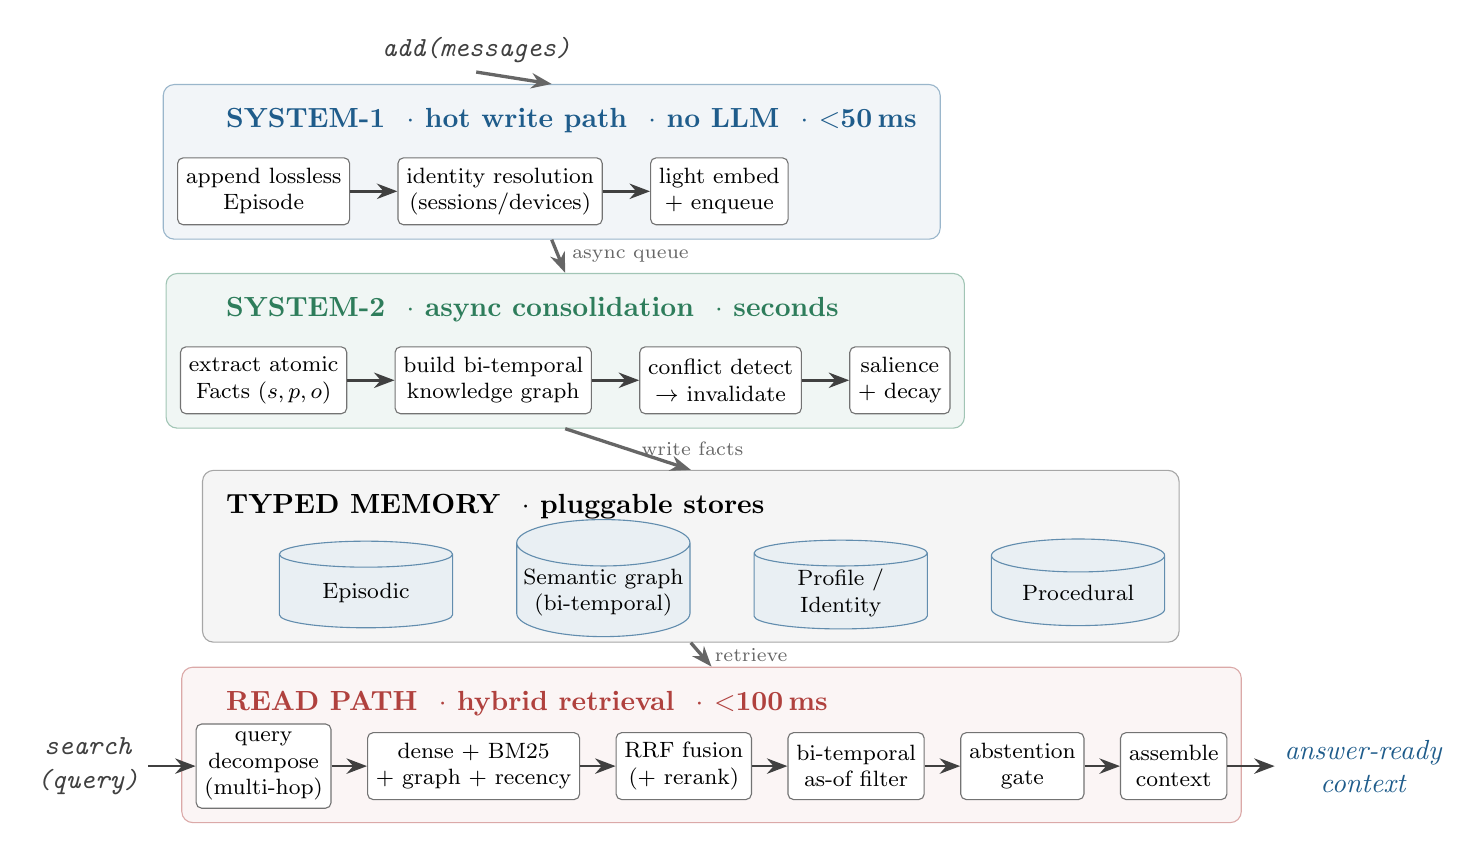
\begin{tikzpicture}[
  font=\footnotesize,
  chip/.style={rounded corners=2pt, draw=black!55, fill=white, inner sep=3pt,
               minimum height=8.5mm, align=center},
  store/.style={cylinder, shape border rotate=90, aspect=0.28, draw=engramblue!70,
                fill=engramblue!10, minimum height=11mm, minimum width=22mm, align=center,
                inner sep=1pt},
  io/.style={font=\itshape, text=black!75, align=center},
  ttl/.style={font=\bfseries, anchor=west},
  >={Stealth[length=2.6mm]},
  flow/.style={->, line width=1pt, draw=black!75},
  vflow/.style={->, line width=1.2pt, draw=black!60},
]
% ----- input -----
\node[io] (in) at (3.0,10.2) {\texttt{add(messages)}};
% ----- SYSTEM-1 -----
\node[ttl, text=engramblue] (t1) at (-0.3,9.3) {SYSTEM-1 \ $\cdot$\ hot write path \ $\cdot$\ no LLM \ $\cdot$\ $<$50\,ms};
\node[chip] (s1a) at (0.3,8.4) {append lossless\\Episode};
\node[chip, right=6mm of s1a] (s1b) {identity resolution\\(sessions/devices)};
\node[chip, right=6mm of s1b] (s1c) {light embed\\$+$ enqueue};
\draw[flow] (s1a)--(s1b); \draw[flow] (s1b)--(s1c);
% ----- SYSTEM-2 -----
\node[ttl, text=s2green] (t2) at (-0.3,6.9) {SYSTEM-2 \ $\cdot$\ async consolidation \ $\cdot$\ seconds};
\node[chip] (s2a) at (0.3,6.0) {extract atomic\\Facts $(s,p,o)$};
\node[chip, right=6mm of s2a] (s2b) {build bi-temporal\\knowledge graph};
\node[chip, right=6mm of s2b] (s2c) {conflict detect\\$\to$ invalidate};
\node[chip, right=6mm of s2c] (s2d) {salience\\$+$ decay};
\draw[flow] (s2a)--(s2b); \draw[flow] (s2b)--(s2c); \draw[flow] (s2c)--(s2d);
% ----- TYPED MEMORY -----
\node[ttl] (t3) at (-0.3,4.4) {TYPED MEMORY \ $\cdot$\ pluggable stores};
\node[store] (m1) at (1.6,3.3) {Episodic};
\node[store, right=8mm of m1] (m2) {Semantic graph\\(bi-temporal)};
\node[store, right=8mm of m2] (m3) {Profile /\\Identity};
\node[store, right=8mm of m3] (m4) {Procedural};
% ----- READ PATH -----
\node[ttl, text=baselinered] (t4) at (-0.3,1.9) {READ PATH \ $\cdot$\ hybrid retrieval \ $\cdot$\ $<$100\,ms};
\node[chip] (r1) at (0.3,1.1) {query\\decompose\\(multi-hop)};
\node[chip, right=4.5mm of r1] (r2) {dense $+$ BM25\\$+$ graph $+$ recency};
\node[chip, right=4.5mm of r2] (r3) {RRF fusion\\($+$ rerank)};
\node[chip, right=4.5mm of r3] (r4) {bi-temporal\\as-of filter};
\node[chip, right=4.5mm of r4] (r5) {abstention\\gate};
\node[chip, right=4.5mm of r5] (r6) {assemble\\context};
\draw[flow] (r1)--(r2); \draw[flow] (r2)--(r3); \draw[flow] (r3)--(r4);
\draw[flow] (r4)--(r5); \draw[flow] (r5)--(r6);
\node[io, left=6mm of r1] (q) {\texttt{search}\\\texttt{(query)}};
\draw[flow] (q)--(r1);
\node[io, right=6mm of r6, text=engramblue] (out) {answer-ready\\context};
\draw[flow] (r6)--(out);
% ----- background bands -----
\begin{scope}[on background layer]
\node[rounded corners=4pt, fill=engramblue!6, draw=engramblue!45, fit=(t1)(s1a)(s1c), inner sep=5pt] (bandS1) {};
\node[rounded corners=4pt, fill=s2green!7, draw=s2green!45, fit=(t2)(s2a)(s2d), inner sep=5pt] (bandS2) {};
\node[rounded corners=4pt, fill=black!4, draw=black!35, fit=(t3)(m1)(m4), inner sep=5pt] (bandM) {};
\node[rounded corners=4pt, fill=baselinered!5, draw=baselinered!45, fit=(t4)(r1)(r6), inner sep=5pt] (bandR) {};
\end{scope}
% ----- vertical flow between bands -----
\draw[vflow] (in.south)--(bandS1.north);
\draw[vflow] (bandS1.south)--node[right=1pt,font=\scriptsize,text=black!60]{async queue}(bandS2.north);
\draw[vflow] (bandS2.south)--node[right=1pt,font=\scriptsize,text=black!60]{write facts}(bandM.north);
\draw[vflow] (bandM.south)--node[right=1pt,font=\scriptsize,text=black!60]{retrieve}(bandR.north);
\end{tikzpicture}%
}
\caption{The \engram{} dual-process architecture: a hot write path (\textsc{System-1}) that never blocks on
an LLM; an asynchronous consolidation path (\textsc{System-2}) that extracts facts, builds the bi-temporal
graph and resolves conflicts non-destructively; a typed memory over pluggable stores; and a hybrid read path
(dense $+$ lexical $+$ graph $+$ recency, fused by RRF) with an as-of filter and an abstention gate.}
\label{fig:arch}
\end{figure}

\subsection{Bi-temporal data model}

Two time axes are first-class everywhere, which is what makes knowledge-updates and ``as-of'' queries
intrinsic rather than bolted-on.

\begin{itemize}
  \item \textbf{Episode} --- a raw, lossless turn/event, stamped with \emph{event time} (when it happened in
  the world) and \emph{ingested-at} (transaction time, when we recorded it).
  \item \textbf{Fact} --- an atomic $(\textit{subject},\textit{predicate},\textit{object})$ claim with surface
  text, an embedding, a \emph{salience} and \emph{confidence}, and \emph{provenance} (the source episode
  ids). It carries two time axes: \emph{valid time} (\texttt{valid\_at} / \texttt{invalid\_at}, when the claim
  is true in the world) and \emph{transaction time} (\texttt{created\_at} / \texttt{expired\_at}, when we
  learned or retracted it), plus a \texttt{supersedes} pointer to the fact it replaces.
  \item \textbf{Entity / Relation} --- graph nodes and edges; edges carry the same bi-temporal stamps.
\end{itemize}

The invariant: \emph{never hard-delete a contradicted fact---invalidate it} (set \texttt{invalid\_at}) and
keep the history. Every fact can therefore answer ``where did this come from?'' and ``what did it replace?''
(Figure~\ref{fig:bitemporal}).

\begin{figure}[t]
\centering
\resizebox{0.8\textwidth}{!}{%
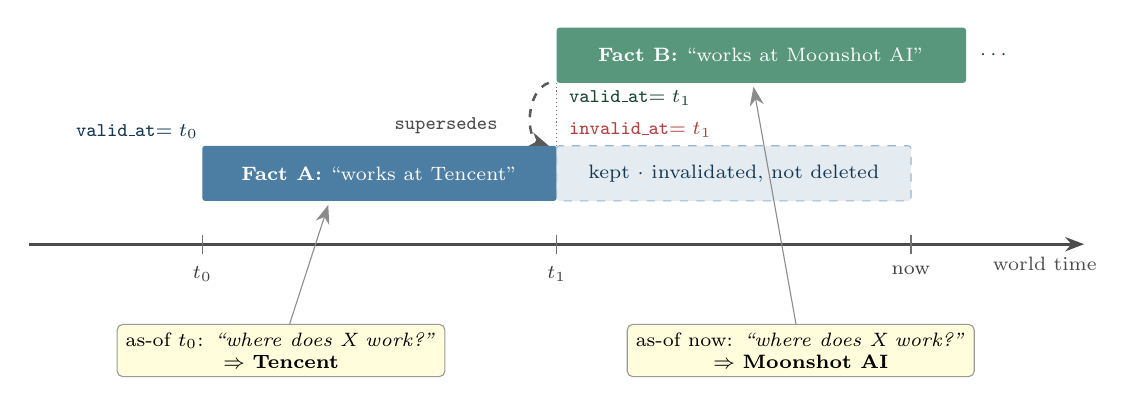
\begin{tikzpicture}[font=\footnotesize, >={Stealth[length=2.4mm]}]
% time axis
\draw[->, line width=1pt, black!70] (-0.2,0)--(13.2,0);
\node[font=\scriptsize, text=black!70, below] at (12.7,-0.04) {world time};
\foreach \x/\lab in {2/{$t_0$}, 6.5/{$t_1$}, 11/{now}}{
  \draw[black!55] (\x,0.12)--(\x,-0.12);
  \node[below, font=\scriptsize, text=black!75] at (\x,-0.16) {\lab};
}
% Fact A: valid in [t0,t1)
\fill[engramblue!80, rounded corners=1pt] (2,0.55) rectangle (6.5,1.25);
\node[white, font=\scriptsize] at (4.25,0.9) {\textbf{Fact A:} ``works at Tencent''};
% Fact A kept-but-invalid in [t1, now]
\draw[fill=engramblue!12, draw=engramblue!45, dashed, rounded corners=1pt] (6.5,0.55) rectangle (11,1.25);
\node[text=engramblue!60!black, font=\scriptsize] at (8.75,0.9) {kept $\cdot$ invalidated, not deleted};
\node[font=\scriptsize, text=engramblue!60!black, above left=-1pt and -2pt] at (2,1.25) {\texttt{valid\_at}$=t_0$};
% Fact B: valid in [t1, ...)
\fill[s2green!80, rounded corners=1pt] (6.5,2.05) rectangle (11.7,2.75);
\node[white, font=\scriptsize] at (9.1,2.4) {\textbf{Fact B:} ``works at Moonshot AI''};
\node[text=s2green!55!black, font=\scriptsize, right] at (11.75,2.4) {$\cdots$};
% supersession instant at t1
\draw[densely dotted, black!55] (6.5,1.25)--(6.5,2.05);
\node[font=\scriptsize, text=baselinered, right=1pt] at (6.5,1.45) {\texttt{invalid\_at}$=t_1$};
\node[font=\scriptsize, text=s2green!55!black, right=1pt] at (6.5,1.86) {\texttt{valid\_at}$=t_1$};
% supersedes arrow B -> A (bowing left of t1)
\draw[->, dashed, line width=0.9pt, black!65] (6.4,2.05) to[out=-160,in=160] (6.4,1.25);
\node[font=\scriptsize, text=black!70, left=5pt] at (6.05,1.5) {\texttt{supersedes}};
% as-of queries
\node[rounded corners=2pt, draw=black!40, fill=yellow!14, font=\scriptsize, align=center, inner sep=3pt]
  (qa) at (3,-1.35) {as-of $t_0$: \emph{``where does X work?''}\\$\Rightarrow$ \textbf{Tencent}};
\node[rounded corners=2pt, draw=black!40, fill=yellow!14, font=\scriptsize, align=center, inner sep=3pt]
  (qb) at (9.6,-1.35) {as-of now: \emph{``where does X work?''}\\$\Rightarrow$ \textbf{Moonshot AI}};
\draw[->, black!45] (qa)--(3.6,0.5);
\draw[->, black!45] (qb)--(9.0,2.0);
\end{tikzpicture}%
}
\caption{Bi-temporal facts make contradictions and ``as-of'' queries first-class: when Fact~B arrives at
$t_1$, \engram{} sets $\text{A.}\texttt{invalid\_at}=t_1$ and $\text{B.}\texttt{supersedes}=\text{A}$---A is
\emph{invalidated, not deleted}, so history and provenance survive---and a point-in-time query resolves
against the fact valid at that time, which is what the knowledge-update and temporal categories require.}
\label{fig:bitemporal}
\end{figure}

\subsection{System-1: the hot write path}

On \texttt{add(messages)}, \engram{} appends a lossless episode, resolves identity (linking a user/entity
across sessions and devices), computes a light embedding, and enqueues the episode for consolidation. No LLM
runs on this path, keeping it within a sub-50ms budget so writes never block the agent.

\subsection{System-2: asynchronous consolidation}

Off the critical path, the consolidation engine (i) extracts atomic facts from episodes (rule-based by
default, LLM-based when a model is configured), (ii) builds the bi-temporal knowledge graph of entities and
relations, (iii) detects conflicts and invalidates superseded facts, and (iv) scores salience and applies
decay/reinforcement so unreinforced memories fade and the store stays small and fast. Hierarchical
abstraction (session summaries $\rightarrow$ profile) runs here as well.

\subsection{Cheap-then-escalate conflict resolution}

When a new fact arrives for an existing $(\textit{subject},\textit{predicate})$ slot with a different object,
\engram{} resolves it in increasing order of cost. First, cheap signals: an exact \textbf{slot match}
signals a likely update, \textbf{embedding similarity} catches the same attribute under a different
free-form predicate, and \textbf{content subsumption} (one claim $\subseteq$ the other) separates
contradiction from elaboration. Second, if the claims are clearly contradictory and temporally ordered, the
old one is invalidated ($\texttt{old.invalid\_at} \leftarrow \texttt{new.valid\_at}$) and
$\texttt{new.supersedes} \leftarrow \texttt{old.id}$---with \emph{no LLM call}. Only genuinely ambiguous cases
escalate to an LLM adjudicator. This is the cost win over systems that invoke an LLM on every fact, while
preserving temporal correctness and a complete audit trail.

\subsection{The hybrid read path}

On \texttt{search(query)}, \engram{} (1) understands the query and, for multi-hop questions, decomposes it
into sub-queries; (2) retrieves in parallel through four complementary channels---dense semantic, BM25
lexical, graph $n$-hop from the query's entities, and recency/salience; (3) fuses the ranked lists with
Reciprocal Rank Fusion~\citep{cormack2009rrf} and an optional cross-encoder rerank over the top-$k$ (off by
default); (4) applies a bi-temporal ``as-of'' filter (what we believed was true at time $T$); (5) passes an
abstention gate that declines to answer when the evidence is absent; and (6) assembles a deduplicated,
provenance-tagged, token-budgeted context. The per-item score combines all signals:
\begin{equation}
\label{eq:score}
\begin{split}
\mathrm{score}(\textit{item} \mid q) ={}&
  w_{\text{sem}}\cos(q,\textit{item})
  + w_{\text{lex}}\,\mathrm{bm25}(q,\textit{item})
  + w_{\text{graph}}\,\mathrm{prox}(\textit{item}) \\
  &{}+ w_{\text{rec}}\,e^{-\Delta t/\tau}
  + w_{\text{sal}}\,\mathrm{sal}(\textit{item}),
\end{split}
\end{equation}
where the weights are configuration-driven and tuned on the harness rather than hand-set. Crucially, the
assembled context is \emph{hybrid}: it contains both the conflict-resolved bi-temporal facts and the most
relevant raw session chunks (plus session-level summaries). \S\ref{sec:results} shows this hybrid composition
is necessary---facts alone lose recall.

Every external dependency---LLM, embedder, vector, graph and lexical store---sits behind an interface with
a zero-dependency offline fallback, so the loop runs with no API keys (Appendix~\ref{app:backends}).

\section{Experimental Setup}
\label{sec:setup}

\paragraph{Benchmark.}
\textsc{LongMemEval}\textsubscript{S}~\citep{wu2025longmemeval}: 500 questions, each over a haystack of
$\sim$50 sessions ($\sim$115k tokens), pulled from the public release. Questions span seven categories
(Figure~\ref{fig:percat}). We grade with the \emph{official} category-specific judge prompts---including the
temporal off-by-one tolerance, knowledge-update old-information tolerance, preference-rubric leniency, the
``contains the answer'' semantics, and unanswerable (abstention) detection---rather than a home-grown judge.

\paragraph{Models.}
Embedder: \texttt{BAAI/bge-small-en-v1.5} (local, no API key). System-2 fact extractor:
\texttt{doubao-seed-1.6-flash}. Answerer: \texttt{doubao-seed-2.0-pro} for the headline, and the small
\texttt{doubao-seed-1.6-flash} as a second backbone (\S\ref{sec:backbones}). Judge: DeepSeek's official API
(\texttt{deepseek-chat}, which served DeepSeek-V4-Flash at the time of the runs), prompted with the official
LongMemEval judge prompts; footnote~\ref{fn:judge} explains why this differs from the arXiv~v1 judge. Models
are addressed as \texttt{provider:model} and resolved via LiteLLM, so any OpenAI-compatible endpoint (OpenAI,
DeepSeek, a local model) can be substituted and the same commands run.

\paragraph{Systems.}
\lean{} (our headline) retrieves a small hybrid slice---conflict-resolved bi-temporal facts $+$ the most
relevant raw session chunks $+$ session summaries---and answers from \emph{that alone} ($\sim$7.9k tokens),
never the full history. \full{} is the baseline: stuff the entire haystack into the prompt ($\sim$79k tokens).
The harness applies the \emph{same answerer and judge to every system}, so any within-run comparison is
apples-to-apples by construction.

\paragraph{Retrieval configuration.}
The hybrid read path fuses five ranked signals by weighted Reciprocal Rank Fusion ($k_{\text{RRF}}=60$) with
the Eq.~\eqref{eq:score} weights $w_{\text{sem}}=1.0$, $w_{\text{lex}}=0.6$, $w_{\text{graph}}=0.8$,
$w_{\text{rec}}=0.3$, $w_{\text{sal}}=0.25$ (the repository defaults in \texttt{engram/config.py}, tuned on
the harness, not hand-set per question). The lean slice assembles up to 8 conflict-resolved facts, the
top-15 fused items, 2 raw session chunks, and 28 session-level summaries; exact flag semantics are in the
reproduce command.

\paragraph{Reproduce.}
The headline run is a single command, given verbatim (with the model identifiers and every flag) in the
Reproducibility Statement; its raw per-question log is committed to the repository as
\texttt{results/run500\_v3\_main\_deepseekjudge.jsonl}. The second backbone swaps the answerer flag and the
LOCOMO slice the data flag, nothing else. \texttt{python eval/report.py <run.jsonl>} recomputes every table
below from a log, and \texttt{python paper/check\_numbers.py} asserts that every number in this paper's
main text equals a value recomputed from the committed logs.

\paragraph{Measurement-integrity notes.}
Six bugs and drifts that silently inflate or deflate memory-benchmark numbers---and that we hit and fixed
ourselves---are documented in Appendix~\ref{app:integrity}: a ``memory'' system that still contained the
full history, a truncated full-context baseline, a home-grown judge stricter than the official one,
abstention grading, retry handling (the headline run has 0 errored questions of 500 under both systems),
and the judge-endpoint drift of footnote~\ref{fn:judge}. They are the reason cross-source numbers disagree.

\section{Results}
\label{sec:results}

\paragraph{Headline.}
Table~\ref{tab:headline} and Figure~\ref{fig:acctokens} report the full 500-question result. \engram{}'s lean
configuration beats the full-context baseline by \textbf{$+5.6$ points} (84.4\% vs.\ 78.8\%) while using
\textbf{10$\times$ fewer tokens} (7.9k vs.\ 79k), with 0 of 500 errored under both. The filtered slice is not
merely cheaper---it is \emph{more accurate} than the full window, consistent with the distractor mechanism
of \citet{liu2024lost}. The margin is statistically significant but not large: across the 500 paired
questions \lean{} is correct on 68 that the baseline misses versus 40 the other way (McNemar's exact test,
$p=0.009$), and a paired bootstrap puts the 95\% CI of the gain at $+1.6$ to $+9.6$ points. All statistics
are recomputed from the committed log by \texttt{paper/compute\_stats.py}.

\begin{table}[h]
\centering
\caption{\textsc{LongMemEval}\textsubscript{S}, 500 questions, official judge prompts; same answerer
(\texttt{doubao-seed-2.0-pro}) and judge (\texttt{deepseek-chat}) for both systems. Accuracy with a Wilson
95\% CI (paired difference: McNemar exact $p=0.009$); latency is end-to-end wall-clock per question
including the remote answerer call, p50\,/\,p95.}
\label{tab:headline}
\resizebox{\linewidth}{!}{%
\begin{tabular}{lcrrr}
\toprule
System & Overall acc.\ (95\% CI) & Avg.\ context tokens & Latency p50\,/\,p95 & Errors \\
\midrule
\textbf{\engram{}} (\lean{}) & \textbf{84.4\%} \,[81.0,\,87.3] & \textbf{7.9k} & 52.9\,s\,/\,118.7\,s & 0 / 500 \\
full-context baseline        & 78.8\% \,[75.0,\,82.2]          & 79.2k         & 14.6\,s\,/\,59.2\,s  & 0 / 500 \\
\bottomrule
\end{tabular}}
\end{table}

\begin{figure}[t]
\centering
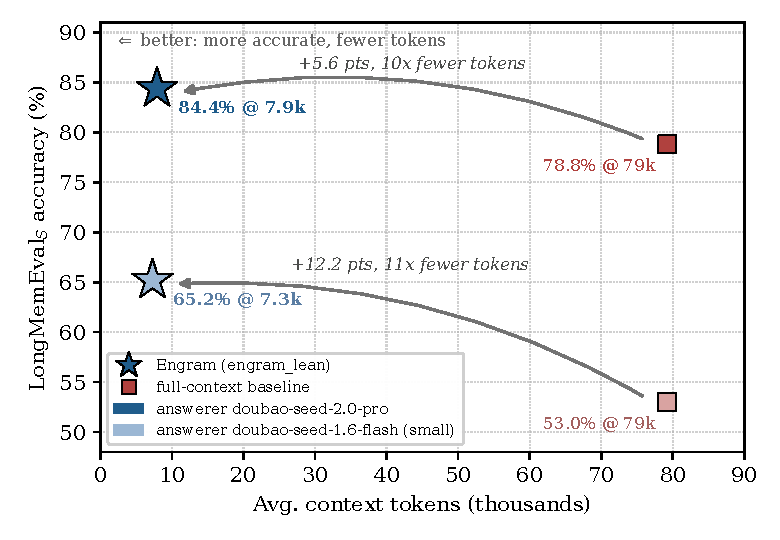
\includegraphics[width=0.62\textwidth]{fig_acc_tokens.pdf}
\caption{Accuracy vs.\ average context tokens on LongMemEval\textsubscript{S} (500 questions) for two answerer
backbones: \lean{} (star) sits up and to the left of full-context (square)---\textbf{$+5.6$ points at
10$\times$ fewer tokens} for \texttt{doubao-seed-2.0-pro}, $+12.2$ at 11$\times$ for the small
\texttt{doubao-seed-1.6-flash} (Table~\ref{tab:backbones}).}
\label{fig:acctokens}
\end{figure}

\paragraph{Per-category.}
Table~\ref{tab:percat} and Figure~\ref{fig:percat} break both systems down by category. The lean slice wins
four of the six categories and ties one. The margins are largest where the full window has the most to
distract from: \emph{single-session-preference} ($+30.0$; a category that is hard field-wide, and where the
baseline reaches only 50.0\%), \emph{multi-session} aggregation ($+11.3$; counting and aggregating across
many sessions, where the baseline mostly abstains) and \emph{single-session-user} ($+8.6$).
\emph{Temporal-reasoning} (date-stamped context $+$ as-of filtering) is a modest $+2.3$. The one loss is
\emph{knowledge-update} ($-6.4$): the baseline sees every version of a changed value in order and applies
``most recent wins'' itself, whereas the lean slice depends on consolidation having attached the update to
the right slot. Of the eight knowledge-update questions the slice loses and the baseline gets, seven end in
a superseded value or an abstention---consistent with the update not reaching the slice, a consolidation
miss rather than a reading error (\S\ref{sec:limitations}). The 30 \emph{abstention} items, graded by the
official \emph{unanswerable} judge and counted inside their host categories above, come out at 90.0\% for
\lean{} vs.\ 93.3\% for the baseline: the abstention gate declines correctly on most of them, at a small
cost against a baseline that, as the error analysis below shows, abstains often anyway.

\begin{table}[h]
\centering\footnotesize
\caption{Per-category accuracy on \textsc{LongMemEval}\textsubscript{S} (500 questions; the run of
Table~\ref{tab:headline}). $\Delta$ is \lean{} minus full-context. The 30 unanswerable (abstention) items are
counted inside their host categories; broken out, they score 90.0\% (\lean{}) vs.\ 93.3\% (full-context).}
\label{tab:percat}
\begin{tabular}{lrrrr}
\toprule
Category & \lean{} & full-context & $\Delta$ & $n$ \\
\midrule
multi-session             & \textbf{78.2\%} & 66.9\%          & $+11.3$ & 133 \\
temporal-reasoning        & \textbf{83.5\%} & 81.2\%          & $+2.3$  & 133 \\
knowledge-update          & 84.6\%          & \textbf{91.0\%} & $-6.4$  & 78 \\
single-session-user       & \textbf{91.4\%} & 82.9\%          & $+8.6$  & 70 \\
single-session-assistant  & 94.6\%          & 94.6\%          & $+0.0$  & 56 \\
single-session-preference & \textbf{80.0\%} & 50.0\%          & $+30.0$ & 30 \\
\midrule
overall                   & \textbf{84.4\%} & 78.8\%          & $+5.6$  & 500 \\
\bottomrule
\end{tabular}
\end{table}

\begin{figure}[t]
\centering
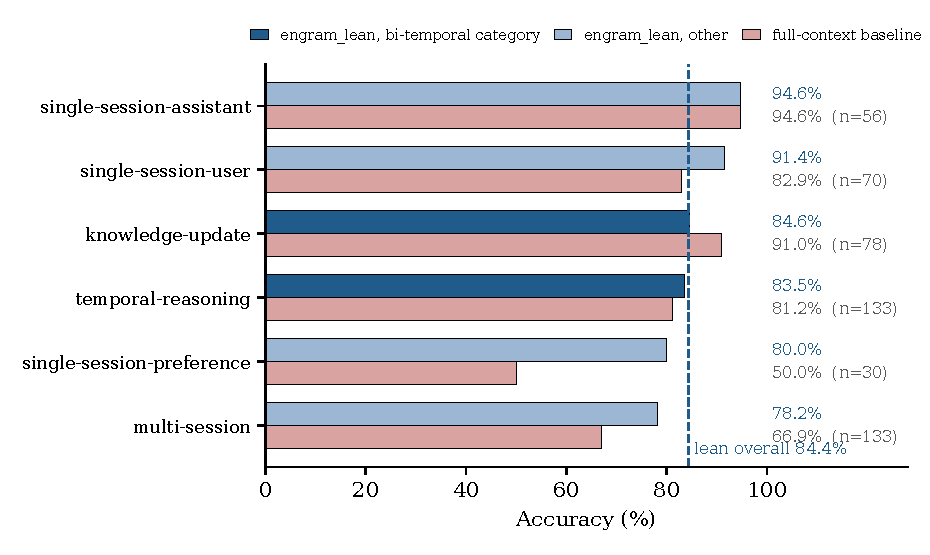
\includegraphics[width=0.74\textwidth]{fig_percat.pdf}
\caption{Per-category accuracy of \lean{} vs.\ full-context on the full 500-question set (dashed line: the
84.4\% lean overall). The two bi-temporal categories are highlighted: temporal-reasoning a small win,
knowledge-update the one loss; the largest margins are single-session-preference and multi-session.}
\label{fig:percat}
\end{figure}

\paragraph{Error analysis: full-context is ``lost in the middle.''}
The two systems fail differently. Of the full-context baseline's 106 errors, \textbf{57\% (60) are
abstentions}---it answers ``I don't know'' even though, by construction, the evidence lies somewhere in its
$\sim$79k-token window; it simply fails to locate it. On the 68 questions where \lean{} is correct and
full-context is wrong, full-context abstains on 59\% (40) and returns a \emph{wrong} value on the other 28.
\lean{}, answering from a $\sim$7.9k-token slice, abstains on 60/500---and 27 of those are among the 30
genuinely unanswerable items. This is the ``lost in the middle'' effect~\citep{liu2024lost} made
quantitative: past a point, more context is \emph{not} more accuracy if the model cannot find the relevant
span (counts recomputed from the committed logs by \texttt{paper/compute\_stats.py}).

\paragraph{The read path must be hybrid.}
A load-bearing finding from development: a \emph{facts-only} read path---answering purely from extracted
$(s,p,o)$ facts---\emph{loses recall} relative to the hybrid path, because extraction drops detail that some
questions need verbatim. Adding the most relevant raw session chunks back alongside the conflict-resolved
facts restores that detail; the facts contribute conflict-resolved, bi-temporal signal and the chunks restore
specificity. The headline configuration is hybrid for exactly this reason, and we caution against shipping
facts-only QA. We report this as a design observation; a controlled facts-only ablation on the full
500-question set under the same judge is reported as future work (\S\ref{sec:limitations}), not claimed here.

\paragraph{Efficiency.}
The retrieved context averages $\sim$7.9k tokens, 10$\times$ leaner than the $\sim$79k full-context
baseline; the saving is in prompt tokens, the quantity that grows with history. End-to-end latency per
question is \emph{higher} for \lean{} (p50 52.9\,s vs.\ 14.6\,s, Table~\ref{tab:headline}). The harness
records wall-clock per question including the remote answerer call and does not instrument retrieval
separately, so we report the latency as measured and make no retrieval-latency claim from these logs.

\subsection{A second backbone: the weaker the reader, the larger the gain}
\label{sec:backbones}

Memory quality should not depend on one model's ability to read our structures, so the same 500 questions
were also run with the answerer swapped for the small \texttt{doubao-seed-1.6-flash}, everything else
unchanged (Table~\ref{tab:backbones}). That run was made in June on the revision of that date and graded by
the judge that has since been retired (footnote~\ref{fn:judge}), so the table names the code revision and
judge per row and we include the June run of the pro answerer as its within-judge sibling; every row is a
within-run, same-judge comparison, which is the claim we make. The lean slice wins under every backbone and
judge, and the margin is \emph{largest for the weakest reader}: $+12.2$ points (65.2\% vs.\ 53.0\%) for the
small answerer, against $+3.0$ for the pro answerer under the same judge and code, and $+5.6$ on the current
code, at a $\sim$10--11$\times$ token ratio throughout. With the small answerer the lean advantage holds in
five of six categories, the exception being single-session-assistant, which is near ceiling for both
(per-category gaps in Appendix~\ref{app:flash}). The reading is simple: a strong model can partly compensate for a
noisy window by searching it; a weak one cannot, so removing distractors is worth more to it. That is the
regime that matters for cheap and local deployments.

\begin{table}[h]
\centering\small
\caption{Answerer backbones on the same 500 questions, extractor and harness (gap $=$ \lean{} $-$
full-context; token ratio $=$ full-context / lean tokens). Each row is a within-run comparison under one
judge; rows differ in code revision and judge as marked, so compare gaps, not levels, across rows. Logs:
\texttt{run500\_v3\_main\_deepseekjudge}, \texttt{headline\_500}, \texttt{bb\_flash} (\texttt{results/*.jsonl}).}
\label{tab:backbones}
\resizebox{\linewidth}{!}{%
\begin{tabular}{llrrrr}
\toprule
Answerer & Code / judge & \lean{} & full-context & Gap & Token ratio \\
\midrule
\texttt{doubao-seed-2.0-pro}   & current / \texttt{deepseek-chat}    & \textbf{84.4\%} & 78.8\% & $+5.6$  & 10.0$\times$ \\
\texttt{doubao-seed-2.0-pro}   & June 2026 / retired ARK judge & \textbf{79.0\%} & 76.0\% & $+3.0$  & 10.9$\times$ \\
\texttt{doubao-seed-1.6-flash} & June 2026 / retired ARK judge & \textbf{65.2\%} & 53.0\% & $+12.2$ & 10.9$\times$ \\
\bottomrule
\end{tabular}}
\end{table}

\subsection{A second benchmark: a 200-item LOCOMO slice}
\label{sec:locomo}

% TODO(locomo-full): the full 1986-item LOCOMO run (results/locomo1986_main_deepseekjudge.jsonl) is in
% flight. When it lands: repoint LOCOMO_SLICE in compute_stats.py, replace the numbers in this subsection
% and in the abstract/related-work mentions, and drop the "slice" labels.
LOCOMO~\citep{maharana2024locomo} is a different regime: ten long multi-session conversations whose full
text is only $\sim$16k tokens, a fraction of a \textsc{LongMemEval}\textsubscript{S} haystack. We converted
its QA pairs into the harness's item format so that the \emph{same} answerer, extractor and judge apply
(its adversarial questions map onto the unanswerable judge), and report the \textbf{first 200 of its 1,986
items}---a slice, labelled as such; the full run is in progress. Table~\ref{tab:locomo} gives the result.
Overall the two systems tie (88.0\% vs.\ 89.0\%, $-1.0$; 0 errors under both) at 3.4k vs.\ 16.2k tokens
($\sim$5$\times$). That the margin shrinks to zero here is the expected behaviour, not a regression: with a
16k-token history there is little for retrieval to remove and the full-context reader is not yet lost. The
lean advantage is a function of how much distracting history there is---clear on the $\sim$79k-token
\textsc{LongMemEval} windows, nil on 16k---and we expect it to grow, not shrink, with history length.

The per-category split carries the information. Two of \engram{}'s design bets get independent evidence:
\emph{adversarial} (the answer is not in the conversation) is 100.0\% vs.\ 91.1\% ($+8.9$, $n=45$)---the
abstention gate declines correctly on every item, where the full-context reader answers some---and
\emph{multi-hop} is 78.6\% vs.\ 71.4\% ($+7.1$, $n=28$), the category the multi-hop query planner targets
and one \textsc{LongMemEval} has no separate label for. Single-hop is within noise ($-3.6$, $n=83$). The
clear loss is \emph{temporal-reasoning} ($-16.2$, $n=37$), and its failures are not retrieval misses but
\emph{date-granularity} errors: gold answers such as ``the week before 9 June 2023'' or ``the first weekend
of August'' come back as a single collapsed timestamp, off by weeks or a month, because fact extraction
reduces a relative time expression to one point on the axis while the full-context reader still sees the
original phrasing. This is a limitation of the current extractor that \textsc{LongMemEval}'s more regular
date annotations did not expose---the concrete value of a second benchmark---and it is the next target for
the bi-temporal model (\S\ref{sec:limitations}).

\begin{table}[h]
\centering\footnotesize
\caption{LOCOMO, first 200 of 1,986 items (a slice; the full run is in progress). Same answerer, extractor
and judge as Table~\ref{tab:headline}; log \texttt{results/locomo200\_main\_deepseekjudge.jsonl}, 0 errors.}
\label{tab:locomo}
\begin{tabular}{lrrrr}
\toprule
Category & \lean{} & full-context & $\Delta$ & $n$ \\
\midrule
single-hop         & 90.4\%           & \textbf{94.0\%} & $-3.6$  & 83 \\
adversarial        & \textbf{100.0\%} & 91.1\%          & $+8.9$  & 45 \\
temporal-reasoning & 78.4\%           & \textbf{94.6\%} & $-16.2$ & 37 \\
multi-hop          & \textbf{78.6\%}  & 71.4\%          & $+7.1$  & 28 \\
open-domain        & \textbf{71.4\%}  & 57.1\%          & $+14.3$ & 7 \\
\midrule
overall            & 88.0\%           & \textbf{89.0\%} & $-1.0$  & 200 \\
avg.\ context tokens & 3.4k           & 16.2k           &         & \\
\bottomrule
\end{tabular}
\end{table}

\section{Discussion and Limitations}
\label{sec:limitations}

Because our thesis is that cross-harness numbers are not comparable, we state the honest scope of the
present evidence rather than a leaderboard ``win'':

\begin{itemize}
  \item \textbf{Two backbones from one family; one full benchmark plus a slice.} The headline is
  \textsc{LongMemEval}\textsubscript{S} with a mid-size and a small answerer from the same model family, and
  the small-answerer run predates the judge migration (\S\ref{sec:backbones}). A frontier-class answerer, a
  re-run of the small answerer under the current judge, and the full 1,986-item LOCOMO set (in progress)
  are the immediate next steps, so that memory quality is shown not to depend on one model's ability to
  read our structures.
  \item \textbf{Where the slice loses.} Knowledge-update on \textsc{LongMemEval} ($-6.4$) and
  temporal-reasoning on LOCOMO ($-16.2$) are the two categories where the full-context reader beats the
  lean slice, and both point at consolidation rather than retrieval: an update the extractor misses leaves a
  stale value in the slice, and a relative time expression collapsed to one timestamp loses the granularity
  the question needs. Fixing extraction, not adding context, is the lever.
  \item \textbf{Small samples mislead.} During development, small slices repeatedly read far above the
  full-set truth; we therefore report \emph{only} full-set numbers on \textsc{LongMemEval}, and label the
  LOCOMO result as a slice.
  \item \textbf{Open categories.} Multi-session aggregation and preference are where headroom remains; the
  multi-hop query planner and tuned bi-temporal conflict resolution are the levers we expect to move them.
  \item \textbf{Single run per configuration; no controlled component ablation yet.} We report one full-set
  run per system and backbone and do not quantify run-to-run variance from answerer stochasticity; the
  paired bootstrap interval ($+1.6$ to $+9.6$) is the honest statement of uncertainty for the headline gap,
  and the full-context baseline's spread across full-set runs under one judge (footnote~\ref{fn:judge})
  suggests that noise band is real. Nor do we report a controlled full-set ablation of the read path's
  components (notably the facts-only vs.\ hybrid comparison of \S\ref{sec:results}, which we state as an
  observation). Both are immediate next work.
\end{itemize}

\section{Conclusion}

\engram{} shows that a precisely retrieved, bi-temporal, hybrid context can beat the full-context baseline
\emph{on accuracy}---$+5.6$ points at 10$\times$ fewer tokens on the full \textsc{LongMemEval}\textsubscript{S}
under the official judge prompts, and $+12.2$ for a small answerer---turning long-term memory from a cost
optimization into a quality improvement. Equally,
we contribute the neutral, reproducible harness that makes such a claim checkable: the official judge baked in,
the full-context baseline in every table, documented measurement-integrity pitfalls, and the raw logs published.
In a field where every number is contested, the trustworthy scoreboard is itself the result. The system, the
harness, and the logs are open source\ifanon{} in a public repository (link withheld for double-blind
review; see the Reproducibility Statement)\else{} at \url{https://github.com/ly-wang19/engram}\fi.

\section*{AI Use Statement}
\label{sec:aiuse}

LLM-based AI coding assistants were used in producing this work, in two ways that we separate explicitly.
First, as engineering tools: they wrote and refactored parts of the \engram{} code base, the evaluation
harness, the statistics and figure scripts, and drafted and edited passages of this manuscript under the
authors' direction. Second, as \emph{measured components}: the answerer, the fact extractor and the judge
are LLMs and are named, with model identifiers, in \S\ref{sec:setup}; they are the object of study, not an
authoring aid. The human authors designed the system and the experiments, ran and checked every run,
verified every number against the committed logs (\texttt{paper/check\_numbers.py}), and take full
responsibility for all claims, text and code in the paper.

\section*{Reproducibility Statement}
\label{sec:repro}

Every number in this paper is produced by the in-repo harness and backed by committed per-question logs
(prediction, gold, correctness, tokens, and latency for every question of every run cited: both answerer
backbones on \textsc{LongMemEval}\textsubscript{S} and the LOCOMO slice), and \texttt{paper/check\_numbers.py}
asserts that every number in the main text equals a value recomputed from those logs. The end-to-end loop and unit
tests run with no API keys and no external services via deterministic offline fallbacks; the benchmark
numbers require an OpenAI-compatible model endpoint for the answerer, extractor, and judge, all configurable.
The model identifiers, embedder, and hyper-parameters are in \S\ref{sec:setup}, and the headline run is
the single command below (log: \texttt{results/run500\_v3\_main\_deepseekjudge.jsonl}):
\begin{list}{}{\leftmargin=1em}\item[]\footnotesize\ttfamily
python eval/bench.py --data s --limit 500 --systems engram\_lean,full\_context \textbackslash\\
\hspace*{1.5em}--answerer volcano:doubao-seed-2-0-pro-260215 --judge deepseek \textbackslash\\
\hspace*{1.5em}--extractor volcano:doubao-seed-1-6-flash-250615 --embedder bge-small \textbackslash\\
\hspace*{1.5em}--reasoning --persona --chunks 2 --topk 15 --extract-k 8 \textbackslash\\
\hspace*{1.5em}--summ-k 28 --n-summaries 28
\end{list}
Substitutions: \texttt{--answerer volcano:doubao-seed-1-6-flash-250615} for the second backbone;
\texttt{--data locomo --limit 200} for the LOCOMO slice (items converted from the public release by
\texttt{eval/locomo.py}). The appendix reproduces every prompt verbatim. The significance tests and
confidence intervals in \S\ref{sec:results} are recomputed from the committed logs by
\texttt{paper/compute\_stats.py}, with no model calls. The code, the harness and the raw logs are
\ifanon in a public repository whose link is withheld for double-blind review and will be given in the
camera-ready version\else at \url{https://github.com/ly-wang19/engram}\fi; the benchmark data
(\textsc{LongMemEval} and LOCOMO) are the public releases.

\section*{Ethics Statement}
\label{sec:ethics}

A long-term memory layer necessarily persists personal data across sessions, which raises real privacy
obligations. Two of \engram{}'s core design choices are mitigations as much as features: \emph{non-destructive
invalidation with full provenance} yields an auditable trail of what was believed, when, and from which
source, and \emph{salience decay} lets unreinforced personal details fade by default. Non-destructive
invalidation is a statement about \emph{contradiction}, not about \emph{erasure}: a contradicted fact is
kept, invalidated, so that the history stays auditable, but the store also exposes explicit deletion---a
single fact, or everything held about a user---so that a ``right to be forgotten'' request is a supported
operation rather than a best-effort one. Because every component has a zero-dependency offline fallback,
\engram{} can run fully locally---no user data need leave the operator's machine---and the AGPL-3.0 license
keeps self-hosted data under the operator's control. The principal risks are the obverse of the benefits: a
memory store concentrates sensitive information and must be secured, access-controlled, and scoped to genuine
consent; and a memory that confidently surfaces a \emph{stale} or \emph{wrong} fact can mislead, which is
precisely why the bi-temporal model and the abstention gate (decline when memory lacks the answer) are
first-class rather than optional. All experiments use the public \textsc{LongMemEval} and LOCOMO releases,
whose conversations are synthetic or already published; no private user data were collected or used.

\bibliographystyle{plainnat}
\bibliography{references}

\appendix
\label{app:start}

\section{Prompts}
\label{app:prompts}

For full reproducibility we reproduce the exact prompts the harness uses, verbatim from the repository
(non-ASCII characters are normalised for typesetting). The \emph{answerer} system prompt (used with
\texttt{--reasoning}; it instructs evidence aggregation, most-recent-wins on conflicts, and abstention
only as a last resort):

\begin{lstlisting}[style=prompt]
You answer the user's question using the provided dated context. The context has two parts: a FACTS
index (a digest) AND the full dated CONVERSATIONS below it. The answer is USUALLY present -- search BOTH
parts thoroughly before concluding anything. The dates are real; use them for temporal reasoning.

DIG FOR THE ANSWER FIRST. Most questions ARE answerable from the history -- your job is to find the
evidence, not to give up. If the FACTS digest doesn't contain it, scan the full CONVERSATIONS below.

WHEN THE QUESTION NEEDS MULTIPLE EVIDENCE PIECES (counting, summing, ordering, date arithmetic, duration,
earliest/latest/most-recent, multi-step lookup, knowledge updated over time):
  EVIDENCE: list EVERY relevant dated item from the context, one per line with its date. Be EXHAUSTIVE
  -- scan the whole history; a missed item makes a count or total wrong. Re-read before finalizing.
  REASON: count distinct items / sum / sort by date / compute the date difference / pick the most recent.
  Show the work in 1-2 lines. For durations compute end_date - start_date explicitly.
  ANSWER: <a single concise final answer -- no reasoning on this line>

FOR DATE/TIME/NUMBER ANSWERS: give the MOST SPECIFIC value the context supports (exact date > month+year
> year; exact duration). Read the exact figure from the text -- don't round (e.g. 27 minutes 45 seconds,
not 28 minutes).

WHEN THE QUESTION ASKS FOR A RECOMMENDATION / PREFERENCE: do NOT refuse, do NOT ask a clarifying question,
do NOT give generic advice. Ground the answer in the user's OWN stated history: name the SPECIFIC people,
places, brands, tools, experiences or constraints they mentioned, and tailor the suggestion to those.

FOR SIMPLE SINGLE-FACT QUESTIONS: go straight to 'ANSWER: <fact>'.

CURRENT-STATE questions ('what is my current/latest X', 'where do I work now'): report ONLY the most
recent value by date and explicitly disregard older, superseded ones. The newest dated statement wins.
When facts conflict, ALWAYS trust the most recent one by date.

ABSTENTION -- a careful LAST resort, only after searching the ENTIRE history (facts AND all conversations)
and the SPECIFIC thing asked is genuinely never stated. Do NOT abstain just because it wasn't in the FACTS
digest. If the question presupposes something the user truly never mentioned, reply exactly 'ANSWER: I
don't know' rather than guessing. Never fabricate a value. The 'ANSWER:' line is REQUIRED.
\end{lstlisting}

\noindent The answer template (the context is the only thing that varies across systems):
\begin{lstlisting}[style=prompt]
Today's date: {qdate}

{context}

Question: {question}
Answer:
\end{lstlisting}

\noindent The System-2 fact-extractor system prompt (a non-English worked example is elided for
typesetting; values are kept in the user's original language, only the predicate is English snake\_case):
\begin{lstlisting}[style=prompt]
You are a precise information-extraction engine for a long-term memory system. From a multi-turn
conversation, extract the atomic, durable facts it states about the user and the people/things they
mention (identities, attributes, preferences, relationships, possessions, goals/plans, and events with
their times). Output ONLY a JSON array of objects, each with keys "subject", "predicate", "object",
"text". Use short snake_case predicates (e.g. works_at, lives_in, favorite_color, owns, married_to,
born_in, visited). Capture PREFERENCES explicitly with predicates like likes, dislikes, prefers, avoids,
allergic_to, favorite_<thing>; for each preference or dislike stated, output a SEPARATE fact. Resolve
first-person ('I','my','me') to the user's name when known, otherwise to "user". Capture a stated name as
{"subject":"user","predicate":"name","object":"<Name>"}. LANGUAGE: keep subject and object VALUES (names,
places, brands, free text) in the SAME language the user used -- do NOT translate them; only the predicate
stays English snake_case. "text" is a natural one-sentence statement in the conversation's language. Do
NOT infer or invent facts that are not stated. If there are no durable facts, output [].
\end{lstlisting}

\noindent We grade with the \emph{official} LongMemEval category-specific judge prompts, reproduced
verbatim so scores are leaderboard-comparable:
\begin{lstlisting}[style=prompt]
[single-session-user / single-session-assistant / multi-session]
I will give you a question, a correct answer, and a response from a model. Please answer yes if the
response contains the correct answer. Otherwise, answer no. If the response is equivalent to the correct
answer or contains all the intermediate steps to get the correct answer, you should also answer yes. If
the response only contains a subset of the information required by the answer, answer no.
Question: {q}   Correct Answer: {a}   Model Response: {r}
Is the model response correct? Answer yes or no only.

[temporal-reasoning]  (as above, plus:)
... do not penalize off-by-one errors for the number of days. If the question asks for the number of
days/weeks/months and the model makes off-by-one errors (e.g., predicting 19 days when the answer is 18),
the model's response is still correct.

[knowledge-update]  (as above, plus:)
... If the response contains some previous information along with an updated answer, the response should
be considered correct as long as the updated answer is the required answer.

[single-session-preference]
I will give you a question, a rubric for desired personalized response, and a response. Answer yes if the
response satisfies the desired response. The model need not reflect all points in the rubric; the response
is correct as long as it recalls and utilizes the user's personal information correctly.

[abstention / unanswerable]
I will give you an unanswerable question, an explanation, and a response. Answer yes if the model correctly
identifies the question as unanswerable (it may say the information is incomplete, or give other
information but not the asked information).
\end{lstlisting}

\section{Measurement-Integrity Notes}
\label{app:integrity}

We document the bugs that silently inflate or deflate memory-benchmark numbers, because they are the reason
cross-source numbers disagree:
\begin{enumerate}
  \item \textbf{Lean, not full-history (the honest test).} An earlier headline prepended facts \emph{above the
  entire history}; because that system \emph{contains} full-context, it cannot really lose to it and does not
  validate the retrieval thesis. The headline is now \lean{}, which answers from a $\sim$7.9k-token retrieved
  slice.
  \item \textbf{Full-context truncation.} The baseline was once capped below the haystack size, feeding it
  only the oldest sessions; this \emph{deflated the baseline}. Fixed so it receives the whole haystack. (Any
  much lower full-context figure from before this fix is a truncation artifact.)
  \item \textbf{Official judge, not a home-grown one.} A generic ``same info?'' judge was \emph{stricter} than
  the official LongMemEval judge and made scores non-comparable; we use the official prompts verbatim.
  \item \textbf{Abstention} questions are graded by the official \emph{unanswerable} judge.
  \item \textbf{Reliability.} The LLM client uses exponential-backoff retry with transient/permanent error
  classification; the headline run completed with \textbf{0 errored questions} of 500 under both systems.
  \item \textbf{Judge endpoint drift.} The judge behind our arXiv~v1 numbers was a third-party endpoint that
  was retired underneath the documented command, and nothing in the repository noticed until the command
  failed; the absolute scores moved when we re-ran under a judge we can still reach
  (footnote~\ref{fn:judge}). A reproducible harness must name its judge beside every number and keep every
  log it cites committed, which is what we now do.
\end{enumerate}

\section{Pluggable Backends}
\label{app:backends}

Every external dependency---LLM, embedder, vector store, graph store, lexical index---sits behind an interface
with a zero-dependency offline fallback (a hashing embedder, a rule-based extractor, in-memory stores). The
end-to-end loop and the unit tests therefore run deterministically with no API keys and no services; real
backends (BGE embeddings, LanceDB/Qdrant/pgvector, Kuzu/Neo4j, any LLM via LiteLLM) slot in behind the same
interfaces.

\section{Second Backbone: Per-Category Gaps}
\label{app:flash}

With the small \texttt{doubao-seed-1.6-flash} answerer (Table~\ref{tab:backbones}; log
\texttt{results/bb\_flash.jsonl}), the lean advantage holds in five of six categories: multi-session
$+16.5$, temporal-reasoning $+15.8$, single-session-user $+12.9$, single-session-preference $+10.0$,
knowledge-update $+9.0$. The exception is single-session-assistant ($-1.8$), which is near ceiling for both
systems. All gaps are \lean{} minus full-context within that run, under its own judge.

\section{Qualitative Examples}
\label{app:examples}

Table~\ref{tab:qual} shows representative cases drawn from the committed headline log
(\texttt{results/run500\_v3\_main\_deepseekjudge.jsonl}) where \lean{} answers correctly and the
full-context baseline does not. Two failure modes recur. \textbf{(i) Lost in the
middle}~\citep{liu2024lost}: the evidence \emph{is} present in full-context's $\sim$79k-token window, yet
it returns ``I don't know,'' while the lean $\sim$7.9k-token slice surfaces it. \textbf{(ii) Wrong value
from a noisy window}: full-context returns a value that is present in the history but is not the one the
question asks for (a stale count, the wrong duration, a neighbouring figure) while the lean slice returns
the current one. These are illustrative, not cherry-picked headline numbers; all per-question records
(prediction, gold, correctness) are in the repository.

\begin{table}[h]
\centering
\footnotesize
\caption{Representative cases from the \textsc{LongMemEval}\textsubscript{S} logs where \lean{} is correct
and full-context is wrong (ID = the benchmark's question id; predictions verbatim, lightly truncated).}
\label{tab:qual}
\begin{tabular}{@{}l p{2.0cm} p{1.9cm} p{2.7cm} p{2.7cm}@{}}
\toprule
ID & Category & Gold & \engram{} (\lean{}) & full-context \\
\midrule
\texttt{69fee5aa} & knowledge-update & 38 & 38 & \emph{37} \\
\texttt{ba61f0b9} & knowledge-update & 6 & 6 & \emph{5} \\
\texttt{0db4c65d} & temporal-reasoning & 18 days & 18 days & \emph{6 days} \\
\texttt{d851d5ba} & multi-session & \$3,750 & \$3750 & \emph{\$8750} \\
\texttt{2311e44b} & multi-session & 190 & 190 pages & \emph{I don't know} \\
\texttt{8ebdbe50} & single-session-user & Data Science & Data Science certification & \emph{I don't know} \\
\bottomrule
\end{tabular}
\end{table}

\end{document}
